\chapter{{Theoretische Grundlagen}} \label{Theorie}

In diesem Kapitel erfolgt eine Auseinandersetzung mit den zentralen Prinzipien, die die theoretische Basis der Studie bilden. Es ist in zwei Bestandteile gegliedert: einerseits in einen Überblick über den aktuellen Forschungsstand, der dazu dient, die Untersuchung im theoretischen Gesamtkontext zu verorten. Andererseits werden die für das Forschungsvorhaben relevanten Konzepte vorgestellt. Vor diesem Hintergrund wird zunächst der Unterschied zwischen deskriptivem und expressivem sprachlichen Gehalt herausgearbeitet und daraufhin vertieft in das Phänomen der lexikalischen Intensivierung eingeführt. Das Ziel des Kapitels ist es also, den theoretischen Rahmen abzustecken, in dem sich die daran anschließenden empirischen {Untersuchungen bewegen}.

\section{Forschungsüberblick} \label{Forschungsüberblick}
Im Anschluss wird die Untersuchung in die aktuelle Forschungslage eingegliedert, wegbereitende Werke und Studien dargelegt und auf bestehende Forschungslücken hingewiesen. Elementar ist dabei die Verknüpfung von Expressivität und Intensivierern, die hier genauer in den Blick {genommen wird.}

Expressivität hat erst innerhalb der letzten drei Dekaden verstärkt Einzug in die formal ausgerichtete sprachwissenschaftliche Literatur gehalten und ist neben den neueren Arbeiten von \citet[]{Gutzmann.2011, Gutzmann.2013a, Gutzmann.2019a} vor allem durch {\citet[]{Kaplan.1997}} und \citet[]{Potts.2007a,Potts.2007b} vertreten: Wie einige Autor:innen zuvor (z.\,B. \citealt[]{Hayner.1956}, \citealt[]{Buehler.1999}, \citealt[]{Jakobson.1960} oder \citealt[]{Cruse.1986}) sieht \citet[]{Kaplan.1997} einen grundlegenden Unterschied im semantischen Modus,
den er am Beispiel der beiden Interjektionen \textit{Ouch} und \textit{Oops} aufzeigt. In diesem Zusammenhang illustriert er, dass es sich bei einem expressiven Sprechakt wie \textit{Ouch} und dessen deskriptiver Paraphrase \textit{I am in pain} nicht nur um zwei unterschiedliche Bedeutungstypen handelt, 
sondern hier ebenso zwei Ausdrucksformen von Information vorliegen: Auch wenn die kommunizierte Information inhaltlich dieselbe ist, wird sie dennoch verschieden ausgedrückt. Auf dieser Grundlage definiert {\citet[]{Potts.2007a,Potts.2007b}} einen Kriterienkatalog, mit dem es möglich ist, die Expressivität von Ausdrücken zu detektieren (vgl. Abschnitt {\REF{Eigenschaften}}). Gleichwohl einige der Kriterien lediglich bedingt haltbar sind, gelten seine Arbeiten zweifellos als Klassiker der Expressivitätsliteratur. {\citet[]{Gutzmann.2011}}, der sich auf die modelltheoretische Semantik von \citet[]{Potts.2005} stützt, nimmt in der Folge erstmals eine binäre Einteilung des Bedeutungstyps von Intensitätspartikeln in deskriptiv und expressiv an, die zentraler Untersuchungsgegenstand dieses Buchs ist.\footnote{Obwohl der Unterschied zwischen \glqq{}stilistisch neutralen, unmarkierten Potenziatoren\grqq{} (\citealt[97]{Suscinskij.1985}) und \glqq{}stilistisch markierten, emotional-expressiven Steigerungswörter[n]\grqq{} (ebd.) schon früher thematisiert wurde, ist \citet[]{Gutzmann.2011} dennoch der Erste, der ihn systematisch auf syntaktischer und semantischer Ebene beschreibt.} In den anschließenden Jahren wurde die theoretische Modellierung von Expressivität an der Syntax-Semantik-Schnittstelle hauptsächlich durch ihn vorangetrieben (vgl. bspw.  \citealt[]{Gutzmann.2015a,Gutzmann.2019a}).

Im Unterschied zu sprachlicher Expressivität fanden lexikalische und morphologisch inkorporierte Intensitätspartikeln frühzeitig in der theoretischen Literatur Beachtung. Hier stellen insbesondere die Arbeiten von {\citet[]{Tobler.1868}}, \citet[]{Hauschild.1899,Hauschild.1929}, \citet[]{Mueller.1899}, {\citet[]{Becher.1907}} und \citet[]{Baumgarten.1908} erste Ansätze dar, die sprachliche Verstärkung im Deutschen systematisch zu erfassen und zu beschreiben. In dieser frühen Phase standen neben der Dokumentation von Kollokationsmöglichkeiten in erster Linie die semantischen Eigenschaften von Steigerungskomposita sowie deren begriffliche Verortung im Vordergrund. Ähnliches wurde von \citet[]{Stoffel.1901} und {\citet[]{Borst.1902}} für das Englische vorgenommen. In den darauffolgenden Arbeiten von \citet[]{Berz.1953}, \citet[]{Sachs.1963} und {\citet[]{Lipka.1966, Lipka.1968}} wird zusätzlich zur semantischen und morphologischen erstmals die etymologische, phonologische und dialektale Komponente, gestützt durch erste empirische Untersuchungen, hinzugezogen. Darauf aufbauend nimmt {\citet[]{Biedermann.1969}} in seiner Dissertation die erste umfangreichere diachrone Klassifikation von Intensitätspartikeln des Deutschen vor, die heute als Meilenstein auf diesem Gebiet gilt. Auf Grundlage seiner korpuslinguistischen Untersuchung bildet er verschiedene semantische Klassen, deren Mitglieder sich abgesehen von ihrer lexikalischen Abstammung auch in Bezug auf den Intensivierungsgrad voneinander unterscheiden. Die von ihm gewählten Korpora decken die Zeitspanne von 1200 bis 1950 ab und erstrecken sich somit über einen umfassenden Zeitraum von 750 Jahren. Zur Illustration des Gebrauchs und der Frequenzen erstellt er einen tabellarischen Katalog, in dem er die von ihm gefundenen Ausdrücke je 150-Jahresintervall zusammenfasst. Ein vergleichbares Wortverzeichnis findet sich in \citet[]{Tobler.1868}. Nachdem sich \citet[]{Bolinger.1972} tiefgehend mit den zugrunde liegenden Mustern der Adjektiv-Intensivierung im Englischen beschäftigt, liefert \citet[]{Os.1989} mit seiner Dissertation das zweite einflussreiche Werk für das Deutsche. In seiner Monografie beschreibt er zahlreiche Intensitätspartikeln, die er gemäß der mit ihnen einhergehenden Intensität in acht Klassen einordnet und hinsichtlich ihrer Kollokationsbedingungen analysiert. Unterstützt wird die Stufenzuweisung der Ausdrücke durch den Bezug auf unterschiedliche Skalentypen, wodurch {\citet[]{Os.1989}} gegenläufig zu {\citet[]{Biedermann.1969}} alle Intensitätsstufen gleichermaßen einschätzen kann und dadurch die bis dahin bestehenden Lücken füllt. Als Ergänzung zu seinen Ausführungen listet er im Anhang etwa 800 seinerzeit vorkommende lexikalische Intensivierer auf, wobei er sowohl intensitätsverstärkende als auch -mindernde Ausdrücke berücksichtigt. Darüber hinaus bezieht er eine Vielzahl von inkorporierbaren adjektivischen und substantivischen Kompositionsgliedern wie \textit{-hart} in \textit{steinhart} oder \textit{Bomben-} in \textit{Bombenleistung} mit ein, die als Bestandteil der Intensivierung auftreten können. Neben der Korpusuntersuchung zur Verstärkung mithilfe entlehnter Präfixe von {\citet[]{Ruf.1996}} präsentiert ebenso {\citet[]{Paradis.1997}} eine korpusgestützte Untersuchung für englische Intensivierer. Bei ihr stehen zusätzlich zu den semantischen Eigenschaften der Ausdrücke intonatorische Besonderheiten im Fokus. {\citet[]{Kirschbaum.2002b}} erörtert in seiner Dissertation daraufhin die metaphorischen und metonymischen Muster, die der Adjektiv-Intensivierung zugrunde liegen. Die Untersuchung geht er korpuslinguistisch synchron wie diachron an. Die von ihm hinzugezogenen Korpora decken den Zeitraum vom 17. bis zum 21. Jahrhundert ab. Auf dieser Basis kommt er zu dem Schluss, dass die Intensivierung im Deutschen per se systematisch ist und die Wahl des Intensivierungsmittels im Wesentlichen von dem betroffenen Skalenbereich abhängt. Daneben ist {\citet[]{Kirschbaum.2002b}} meinem Wissen nach der Erste, der die Entstehung von Intensivierern in die Sprachwandeltheorie einordnet und Kriterien für die permanente, schnelle Entwicklung erarbeitet. Weitere Monografien neueren Datums liefern {\citet[]{Klara.2009}} und {\citet[]{Laitenberger.2016}}: Während erstere im Besonderen an der Akzentuierung von adjektivischen Steigerungskomposita interessiert ist und die erste Akzentstudie seit {\citet[]{Berz.1953}} durchführt, untersucht letztere die semantische Entwicklung von deutschen und russischen Intensivierern kontrastiv mittels Korpora und Wörterbüchern. Dies zeigt, dass es inzwischen eine ganze Reihe an Werken gibt, die sich dem Phänomen der lexikalischen, morphologischen oder seltener auch syntaktischen Intensivierung widmen. Zu erkennen ist ferner, dass sich die Arbeiten vielfach mit der Semantik von Intensitätspartikeln auseinandersetzen, jedoch ohne dass deren semantischer Status bisher empirisch untersucht wurde. Hinzu kommt natürlich eine Vielzahl von Aufsätzen. Als einschlägig für das Deutsche sind neben den eingangs genannten vor allem die Arbeiten von \citet[]{Suscinskij.1981, Suscinskij.1985}, {\citet[]{Hentschel.1998b}}, {\citet[]{Claudi.2006}}, {\citet[]{Breindl.2007}}, {\citet[]{Gutzmann.2012, Gutzmann.2015b}}, \citet[]{Stratton.2020b}, \citet[]{Pheiff.2023} sowie \citet[]{Scheffler.2023} zu nennen.

Es ist festzustellen, dass die hier aufgeführten Arbeiten, von wenigen Ausnahmen abgesehen, vornehmlich theoretischer statt empirischer Natur sind. Demzufolge ist der Forschungsstand diesbezüglich bislang äußerst spärlich, sodass experimentelle Untersuchungen zu Expressivität bis dato ein Desiderat darstellen. Wenn man die Natur von expressiver Bedeutung und deren Unterschiede zu deskriptiver Bedeutung verstehen möchte, kommt man allerdings nicht umhin, dem Phänomen auch empirisch auf den Grund zu gehen. Dies ist meiner Ansicht nach für das allgemeine Verständnis von Expressivität unumgänglich und ein logischer, längst überfälliger Schritt auf diesem Gebiet. Die noch immer vorherrschende Lücke an experimentellen Untersuchungen zu Expressivität zu schließen, ist eines der Hauptziele dieses Buchs. Aufbauend auf der aktuellen Forschungslage unternimmt sie den ersten Versuch, durch eine groß angelegte Untersuchung und eine Kombination aus verschiedenen linguistischen Methoden neue Erkenntnisse in Bezug auf den semantischen Unterschied zwischen deskriptiven und expressiven Intensivierern zu erlangen. Vor diesem Hintergrund wird erstmals einigen in der Literatur zwar postulierten, jedoch nicht mit empirischen Methoden abgesicherten Hypothesen nachgegangen und eine Brücke von den theoretischen Annahmen zur experimentellen Untersuchung von sprachlicher Expressivität geschlagen. Dazu werden die im Anschluss erörterten Schwerpunkte (d.\,h. deskriptiver vs. expressiver sprachlicher Gehalt, Intensitätspartikeln, {Skalentheorie etc.}) insofern berücksichtigt, als sie die theoretische Basis für den Empirieteil des Buchs bilden. Um den Weg zu den experimentellen Untersuchungen zu ebnen, folgt in {\chapref{Korpus}} eine Korpusstudie, die darauf abzielt, das Vorkommen von ausgewählten expressiven Intensivierern über sieben Dekaden hinweg zu begutachten. In diesem Kontext werden synchrone und diachrone Häufigkeitsverteilungen ermittelt, die die Entwicklung der Ausdrücke in einem Textkorpus über einen größeren Zeitraum hinweg repräsentieren. In den {Kapiteln \REF{Experiment0} und \REF{Experimente}} wird die korpuslinguistische Perspektive um eine experimentelle erweitert. In ersterem Kapitel werden die im Rahmen der Korpusanalyse untersuchten Intensivierer zunächst relativ zueinander in Beziehung gesetzt, während in letzterem eine Stichprobe aus deskriptiven und expressiven Intensivierern kontrastiert wird. Im Fokus der Untersuchungen steht jeweils die Bestimmung des Grades der mit den Ausdrücken assoziierten Skalarität und Sprechereinstellung.

\section{Begriffsklärungen}
Die nachfolgenden Abschnitte befassen sich mit den elementaren Begriffen, die im Kontext der lexikalischen Intensivierung von Bedeutung sind. Sie verfolgen den Zweck, eine tragfähige begriffliche Grundlage zu schaffen, von der die empirischen Untersuchungen gestützt werden können. Dazu erfolgt zunächst eine genauere Begutachtung des Phänomens der sprachlichen Expressivität, an die sich die Funktionsklasse der {Intensitätspartikeln anschließt}.

\subsection{Deskriptiver versus expressiver sprachlicher Gehalt} \label{DeEx}
Expressivität ist in jüngster Zeit zu einem stark diskutierten Thema in der formal orientierten Linguistik avanciert, das je nach Forschungsschwerpunkt aus verschiedenen Blickwinkeln betrachtet wird. Dabei wird im Wesentlichen davon ausgegangen, dass es einen fundamentalen Unterschied im semantischen Modus, d.\,h. zwischen deskriptivem und expressivem Gehalt, gibt, dem sich Sprecher während der Kommunikation bewusst sind. Der Unterschied liegt darin, dass ersterer reine Beschreibungen von (potenziellen) Situationen, Handlungen und Sachverhalten darstellt, wohingegen letzterer in der Regel zur Versprachlichung von subjektiven Einstellungen, Bewertungen und Emotionen dient. Dies wird an zwei klassischen Beispielen von \citet[]{Kaplan.1997} demonstriert.\footnote{Sofern nicht anders angegeben, werden Beispielsätze immer in ihrer Ursprungssprache wiedergegeben.}

 \ea  \label{kap}
 \ea I am in pain. \label{kap1}
 \ex Ouch! \label{kap2}
 \z
 \z

 \ea  \label{kap3}
 \ea I have just observed a minor mishap. \label{kap4}
 \ex Oops! \label{kap5}
 \z
 \z

\noindent Während es sich bei den Sätzen \REF{kap1} und \REF{kap4} um reine Tatsachenbeschreibungen handelt, bringen \REF{kap2} und \REF{kap5} den affektiven Zustand oder Gemütszustand des Sprechers -- in Beispiel \REF{kap} Schmerzen und in \REF{kap3} möglicherweise \mbox{(Fremd-)}Scham oder Überraschung -- unmittelbar zum Ausdruck. Somit sind Expressiva emotiv-evaluativer Natur und für gewöhnlich mit einem erhöhten Grad an Affektivität verbunden (vgl. u.\,a. \citealt[274]{Cruse.1986}; \citealt[189]{Kirschbaum.2002b}; \citealt[44f.]{Loebner.2002};; \citealt[]{Athanasiadou.2007}; \citealt[10]{Gutzmann.2015a}; \citealt[1]{dAvis.2019b}). Nach \citet[151]{Zifonun.1997} handelt es sich bei ihnen um \glqq{}Äußerungen, deren Zweck primär darin besteht, mit einem Gegenstand oder Sachverhalt verbundene Empfindungen des Sprechers kommunikativ zugänglich zu machen\grqq{}. Ebensolche Äußerungen sind deswegen erforderlich, da Gemütsbewegungen und innere Zustände lediglich introspektiv wahrnehmbar und für den Adressaten nicht auf direktem Weg beobachtbar sind {\citep[vgl.][44]{Schwarz-Friesel.2013}}. In der Folge ist man als Gesprächsteilnehmer darauf angewiesen, dass der Interaktionspartner sein Inneres mittels Sprache offenbart. Als subjektive Einstellungsbekundungen liefern Expressiva also Informationen über die inneren Zustände, Einstellungen und Bewertungen des Sprechers, die dem Adressaten andernfalls verborgen blieben. Hierin unterscheiden sie sich von rein neutralen Sachverhaltsbeschreibungen: Expressiva beschreiben innere Zustände nicht, sondern sie bringen sie schlicht freiweg zum Ausdruck {\citep[vgl.][485]{Gutzmann.2018}}. Aus diesem Grund gibt es in Sprachen zahlreiche Möglichkeiten, innere Empfindungen zu externalisieren und für das Gegenüber nachvollziehbar zu machen. Daneben zielt ein expressiver Sprachgebrauch darauf ab, mithilfe einer besonderen sprachlichen Ausdruckskraft den größtmöglichen kommunikativen Effekt zu erzielen, glaubwürdig zu erscheinen und für seine Gefühle einzustehen {\citep[vgl.][189ff.]{Kirschbaum.2002b}}. Typischerweise werden diesbezüglich vorrangig Interjektionen, Fluch- und Schimpfwörter oder Intensivierungen genannt. Letztere dienen dazu, den im Satz beschriebenen Sachverhalt auf einer Skala höher zu verorten und dadurch bemerkenswerter zu machen. Hierfür weisen Sprachen die unterschiedlichsten Strategien auf: So können Lexeme durch semantisch inhärent stärkere ersetzt \REF{Ex1} oder verstärkende Partikeln bzw. Präfixoide hinzugefügt \REF{Ex2}, aber auch Stilfiguren wie Metaphern \REF{Ex3}, emphatische Exklamativsätze \REF{Ex4} oder Reduplikation \REF{Ex5} verwendet werden, um einer Äußerung zusätzliche pragmatische Schlagkraft zu verleihen.\footnote{Beispielsätze, die sich auf die fiktiven Charaktere der beiden US-Sitcoms \textit{The Big Bang Theory} und \textit{How I met your Mother} beziehen, stammen hier und im Folgenden ausnahmslos von mir.}

\ea  \label{Ex1}
\ea Penny: \glqq{}Das Vorsprechen war \textbf{gut}!\grqq{}
\ex Penny: \glqq{}Das Vorsprechen war \textbf{großartig}!\grqq{}
 \z
 \z

\ea  \label{Ex2}
\ea Amy: \glqq{}Sheldon ist \textbf{klug}.\grqq{}
\ex Amy: \glqq{}Sheldon ist \textbf{sehr klug}.\grqq{}
\ex Sheldon: \glqq{}Flash ist \textbf{schnell}.\grqq{}
\ex Sheldon: \glqq{}Flash ist \textbf{blitzschnell}.\grqq{}
 \z
 \z

\ea  Rajesh: \glqq{}Der Wespenstich \uline{brennt wie Feuer}.\grqq{} \label{Ex3}
\z

\ea  Howard: \glqq{}\uline{Wie heiß Penny doch ist!}\grqq{} \label{Ex4}
\z

\ea   Leonard: \glqq{}Ich habe heute ein \textbf{richtig, richtig} gutes Paper gelesen.\grqq{} \label{Ex5}
\z

\noindent In der schriftlichen Kommunikation kann Intensivierung darüber hinaus durch typografische Besonderheiten wie Versalien \REF{Ex6}, Emojis \REF{Ex7} bzw. Emoticons \REF{Ex8} oder den Einsatz multipler Vokalgrapheme \REF{Ex9} realisiert werden. Sie kann also grundsätzlich von morphologischer, syntaktischer und lexikalischer Natur sein.

\ea  Bernadette: \glqq{}Die Party war \textbf{MEGA}!\grqq{} \label{Ex6}
\z

\ea  Kripke: \glqq{}Sheldon ist ein richtiger Idiot \textbf{\Laughey}\,!\grqq{} \label{Ex7}
\z

\ea  Bert: \glqq{}Amy und ich treffen uns morgen \textbf{:-)}\,.\grqq{} \label{Ex8}
\z

\ea  Stuart: \glqq{}Das Comicbuch ist \textbf{seeehr} gut!\grqq{} \label{Ex9}
\z

\noindent In der mündlichen {(Face-to-Face-)}Kommunikation stehen mit intonatorischen, prosodischen und nonverbalen Mitteln noch weitere Optionen zur Verstärkung bereit (vgl. {\citealt[10]{Paradis.1997}}; {\citealt[187]{Liebrecht.2019}}; {\citealt[2]{Scheffler.2023}}).\footnote{All diese Intensivierungsformen sind zweifelsohne von großer Bedeutung und verdienen eine vertiefte eigenständige Untersuchung. Da im vorliegenden Buch jedoch der semantische Unterschied zwischen deskriptiven und expressiven Intensivierern im Mittelpunkt steht, wird an dieser Stelle auf eine weitere Ausführung verzichtet.}

Im Fokus der Untersuchung steht die lexikalische Intensivierung, bei der ein graduierbares Prädikat
durch eine Intensitätspartikel wie \textit{furchtbar}, \textit{sehr} oder \textit{super} modifiziert wird, vom Ziel des Sprechers geleitet, die bezeichnete Eigenschaft funktional zu verstärken. Um sukzessive tiefer in die Thematik einzutauchen, wird im nächsten Abschnitt abgesehen von einer begrifflichen Einordnung die für dieses Buch gültige Definition präsentiert.

\subsubsection{Expressivität -- Begriffliche Einordnung und Arbeitsdefinition} \label{Arbeitsdefinition}
Das Konzept der Expressivität dient in der Linguistik vor allem dazu, eine Relation zwischen der Sprache als Mittel der menschlichen Kommunikation und der Emotion als psychologisch-physiologischem Phänomen herzustellen (vgl. u.\,a. \citealt[1]{dAvis.2019b}; \citealt[2]{Scheffler.2023}). Vor diesem Hintergrund wird an der Schnittstelle zwischen Semantik und Pragmatik eine Dichotomie angenommen, bei der sich deskriptive und expressive Bedeutung gegenüberstehen: Während erstere grob gefasst die Wirklichkeit beschreibt, wird die expressive Bedeutung oftmals ex negativo als all das definiert, was nicht Teil des deskriptiven Gehalts ist. In der Literatur fallen hierunter zumeist subjektive Bewertungen, Einstellungen und Haltungen. 

 Hier werden zunächst zentrale formal-semantische Ansätze des Expressivitätsbegriffs dargelegt, aus denen im Anschluss eine Arbeitsdefinition abgeleitet wird. Die vorgenommene theoretische Schwerpunktsetzung resultiert aus dem erkenntnisleitenden Interesse, das der Untersuchung zugrunde liegt. Entsprechend werden bloß jene Ansätze beleuchtet, die zum Forschungsvorhaben und zur Beantwortung der zur Diskussion stehenden Annahmen beitragen.

Die in der Literatur häufig besprochene binäre Einteilung in deskriptiven und expressiven Bedeutungsgehalt geht in der Semantik neben den klassischen semiotischen Kommunikationsmodellen von \citet[]{Buehler.1999} und \citet[]{Jakobson.1960} im Kern auf \citet[]{Hayner.1956} zurück, der angesichts der Wechselwirkung zwischen Sprache und Emotion Folgendes konstatiert:

\begin{quotation} \noindent Hence, for the sake of clarity, we probably ought to reserve the terms `true' and `false' for symbolism which `describes' or `indicates' and to use some other terms, such as `clear,' `correct,' `adequate,' etc., for symbolism which `expresses.' Only confusion results when the labels `true' and `false' are appended to signs whose meaning lies exclusively, or primarily, in the dimension of expressiveness. \hfill (\citealt[155]{Hayner.1956})  \end{quotation}
  

\noindent Doch wie äußert sich dieser semantische Unterschied und welcher Nutzen lässt sich daraus für eine adäquate Definition von sprachlicher Expressivität ziehen? Diesen Fragen wird nachfolgend auf den Grund gegangen.\footnote{Dabei ist zu beachten, dass in diesem Abschnitt zunächst als Einführung die grundlegenden Eigenschaften von Expressivität behandelt werden, bevor diese in Abschnitt \ref{Intensivierertypen} auf Intensivierer angewandt werden.}

Den Unterschied zwischen deskriptiver und expressiver Bedeutung erläutert \citet[319f.]{Lang.1983} in Form der beiden Konzepte \textsc{say} (\textit{sagen, dass\,\dots}) und \textsc{express} (\textit{ausdrücken, dass\,\dots}), die sich auf propositionale bzw. nicht-propositionale mentale Repräsentationen beziehen: Ist \textsc{say} als eine reine Sachverhaltsbeschreibung zu verstehen, so drückt \textsc{express} ferner eine evaluative Einstellungsbekundung des Sprechers aus \citep[vgl.][315]{Lang.1983}. Der beschriebene Unterschied wird in Beispiel \REF{nobel} exemplifiziert.

 \ea  \label{nobel}
 \ea Kripke: \glqq{}Sheldon hat den Nobelpreis gewonnen.\grqq{} \label{nobel1}
 \ex Kripke: \glqq{}\textbf{Bedauerlicherweise} hat dieser \textbf{blöde} Sheldon den Nobelpreis gewonnen.\grqq{} \label{nobel2}
 \z
 \z
In Satz \REF{nobel1} wird der Sachverhalt, dass Sheldon den Nobelpreis gewonnen hat, von Kripke wertungsfrei wiedergegeben. {In Satz \REF{nobel2}} äußert Kripke mittels der expressiven Ausdrücke \textit{bedauerlicherweise} und \textit{blöde} daneben auch, dass er den Sieg Sheldons aus irgendwelchen Gründen verurteilt bzw. er ihm den Sieg nicht gönnt. Somit beinhaltet die zweite Äußerung ergänzend zur Sachverhaltsbeschreibung eine emotional-expressive Wertung des Sprechers, die über den deskriptiven Informationsgehalt hinausgeht. Vor diesem Hintergrund inspiziert {\citet[333f.]{Lang.1983}} die Aufrichtigkeitsbedingungen, die den Konzepten \textsc{say} und \textsc{express} zugrunde liegen. Zur Illustration bedient er sich am Unterschied von Lügen und Heucheln: Bei einer Lüge handelt es sich um eine willentliche Täuschung, bei der ein gegebener Sachverhalt in behauptender Weise realitätsfern dargestellt wird. Diese betrifft den propositionalen Gehalt und folglich das Konzept \textsc{say}. Im Falle von Heucheln wird vom Sprecher dagegen eine (vom Adressaten mitunter erwartete) subjektive Einstellung willentlich vorgetäuscht. Die simulierte Einstellung tangiert nicht die propositionale Ebene des Gesagten und ist daher mit dem Konzept \textsc{express} verbunden \citep[vgl.][334]{Lang.1983}. Daher kann Kripke Sheldon gegenüber zwar Freude in Anbetracht des Nobelpreisgewinns heucheln, allerdings kann er ihn diesbezüglich nicht anlügen.

Ähnlich wie \citet[]{Lang.1983} sieht \citet[]{Kaplan.1997} den Unterschied zwischen der deskriptiven und expressiven Information eines (komplexen) sprachlichen Ausdrucks darin, dass erstere propositional bzw. sachverhaltsbeschreibend und wahrheitswertfähig ist, wohingegen dies auf letztere nicht zutrifft. Auch ihm zufolge dienen deskriptive Äußerungen vornehmlich dazu, (mögliche) Situationen, Konzepte oder Objekte in der Welt logisch, d.\,h. objektiv und wertungsfrei, zu kategorisieren: \glqq{}A descriptive is an expression which describes something which either is or is not the case.\grqq{} (\citealt[4]{Kaplan.1997}). Solche Beschreibungen sind auf Wahrheitsebene zu interpretieren, was bedeutet, dass die in der Äußerung offengelegte Sachlage grundsätzlich wahr oder falsch sein kann: \glqq{}[A]n expression is descriptively correct if what it describes is the case\grqq{} ({\citealt[5]{Kaplan.1997}}). Somit ist die Proposition von Kripkes Aussage in \REF{nobel1} \textit{Sheldon hat den Nobelpreis gewonnen} gemäß dem logischen Bivalenzprinzip\footnote{Dem Prinzip der Zweiwertigkeit liegt die folgende semantische Annahme zugrunde: \glqq{}Jede Aussage ist entweder wahr oder falsch\grqq{} (\citealt[17]{Schurz.2018}); eine dritte Möglichkeit gibt es in der traditionellen Logik nicht.} genau dann wahr, wenn Sheldon tatsächlich den Nobelpreis gewonnen hat {(P = $1$)}, während sie hingegen falsch ist, wenn der Sachverhalt im beschriebenen Kontext
nicht zutrifft {(P = $0$}). Oder technisch ausgedrückt: \glqq{}[A] sentence \textit{$\alpha$} means that p just in case \textit{$\alpha$} is true in situation \textit{v} iff \textit{p}, where p is some sentence of our metalanguage that gives the truth conditions for \textit{$\alpha$}.\grqq{} ({\citealt[148]{Chierchia.1990}}).\footnote{Hervorhebungen in Zitaten entstammen, sofern nicht anders angegeben, hier und im weiteren Verlauf stets dem Original.} Demnach ist die Bedeutung deskriptiver Ausdrücke relevant für die logischen Wahrheitsbedingungen (d.\,h. die Wahrheit oder Falschheit) eines Aussagesatzes und in der Folge ebenso in der Lage, dessen Wahrheitsgehalt umzukehren. Dies bezeichnet \citet[11:40]{Kaplan.2004} als \glqq{}semantics of Meanings\grqq{}.

Bei Ausdrücken mit expressivem Gehalt ist dies jedoch nicht der Fall, was den Unterschied zwischen beiden Bedeutungstypen markiert: Da Expressiva in der Regel eine Gemütsverfassung, Einstellung oder Bewertung des Sprechers wiedergeben, können sie nicht wahrheitsfunktional sein: \glqq{}[E]xpressives display something about a state or attitude of the agent.\grqq{} (\citealt[5]{Kaplan.1997}). Aufgrund des Umstands, dass es sich dabei um interne Zustände eines Individuums handelt, ist die Semantik expressiver Ausdrücke nicht über den philosophischen Wahrheitsbegriff modellierbar, was im Einklang mit den Ausführungen von \citet[155]{Hayner.1956} und {\citet[333]{Lang.1983}} steht. Laut {\citet[]{Kaplan.1997}} ist stattdessen vielmehr die Korrektheit oder Angemessenheit im Ausdruck einschlägig: \glqq{}[A]n expression is expressively correct if what it expresses or displays is the case (or, if we take what it expresses or displays to be a state, if the agent indeed is in that state).\grqq{} {(\citealt[5]{Kaplan.1997})}.
Infolgedessen lässt sich der expressive Gehalt nur durch den pragmatischen Gebrauch der betreffenden Ausdrücke beschreiben, was {\citet[11:40]{Kaplan.2004}} \glqq{}semantics of Use\grqq{} nennt. Aus den beschriebenen gebrauchsfunktionalen Gründen setzt \citet[57]{Cruse.2004} die unmittelbare Wirkung von Expressiva mit Katzenschnurren oder dem Schreien eines Babys gleich.

Es ist also zu erkennen, dass sich die Auffassungen von \citet[]{Lang.1983} und {\citet[]{Kaplan.1997}} inhaltlich nicht fundamental voneinander unterscheiden, ist bei beiden doch die Trennung in Externa und Interna ein zentraler Aspekt. Da letzteren grundsätzlich kein Wahrheitswert zugeordnet werden kann und diese somit nicht über den Begriff der logischen Wahrheit analysierbar sind, müsse in diesem Kontext eine Abkehr von der logisch-semantischen Wahrheitstheorie stattfinden, wie \citet[2]{dAvis.2019b} erklären. Den Autor:innen nach macht die  Subjektivität von Interna eine wahrheitsunabhängige, gebrauchsfunktionale Semantik erforderlich, durch die die bis dahin schwer fassbare Semantik von expressiver Bedeutung mit logischen Mitteln exhaustiv beschrieben und modelliert werden kann. Hierfür verweisen sie auf {\citet[]{Kaplan.2004}}, der diese Idee anhand folgender Aussage veranschaulicht:

\begin{quotation} \noindent So, here’s my method: I don’t ask what the expression means, for example, I don’t ask, "'What does \textit{goodbye} mean?'' Instead I ask, what are the conditions under which the expression would be correctly or accurately used? This seems a much more fruitful line of inquiry for a word like \textit{goodbye}. To the degree that such conditions reflect linguistic convention, the information that such a condition obtains is carried in the semantics of
the expression. \hfill (\citealt[14:33]{Kaplan.2004})  \end{quotation}

\noindent Dementsprechend sind bei Interna in erster Linie die Bedingungen relevant, unter denen die Äußerung korrekt, d.\,h. adäquat gebraucht, ist. Auf dieser Grundlage formulieren \citet[7]{dAvis.2019b} zwei hierbei vordergründige Fragen, die auf die Wahrheit deskriptiver Bedeutung (i) und die Korrektheit expressiver Bedeutung (ii) abzielen:

\renewcommand{\labelenumi}{\roman{enumi}.}
\begin{enumerate}
\item Wann ist ein Satz wahr? \par $\rightarrow$ deskriptive, wahrheitsfunktionale Bedeutung
\item Wann ist ein Satz mit expressiven Bedeutungskomponenten korrekt gebraucht? \par $\rightarrow$ expressive, gebrauchsfunktionale Bedeutung
\end{enumerate}

\noindent Angewandt auf Satz \REF{nobel2} im obigen Beispiel bedeutet dies, dass die Proposition von Kripkes Aussage \textit{{Bedauerlicherweise} hat dieser {blöde} Sheldon den Nobelpreis gewonnen} deskriptiv genau dann wahr ist, wenn Sheldon den Nobelpreis gewonnen hat (P = $1$) und expressiv angemessen ist, wenn Kripke wirklich eine Abneigung gegenüber Sheldon hegt {(E = \ding{51})}. Die {Wahrheitsbedingungen (\textit{t} = `truth')} und {Gebrauchsbedingungen (\textit{u} = `use')} der beiden Sätze aus Beispiel \REF{nobel} lassen sich inklusive ihrer Semantik in Anlehnung an {\citet[20f.]{Gutzmann.2015a}} folgendermaßen illustrieren:

\ea
\glqq{}Sheldon hat den Nobelpreis gewonnen\grqq{}\\
ist \uline{wahr},\\
wenn Sheldon tatsächlich den Nobelpreis gewonnen hat. 

\ \ \ \ \ \ \ \ \ \ \ $\lsem$Sheldon hat den Nobelpreis gewonnen$\rsem$\textsuperscript{\textit{t}} =

 \hfill $\lbrace${\textit{w}\,|\,Sheldon hat den Nobelpreis gewonnen in \textit{w}}$\rbrace$
\z

\ea
\glqq{}Bedauerlicherweise hat dieser blöde Sheldon den Nobelpreis gewonnen\grqq{} \\
ist \uline{wahr},\\
wenn Sheldon tatsächlich den Nobelpreis gewonnen hat, \\
und \uline{korrekt gebraucht},\\
wenn der Sprecher eine Abneigung gegenüber Sheldon hat. 
 
  \hfill \ \ \ \ \ \ \ \ $\lsem$Bedauerlicherweise hat dieser blöde Sheldon den NP gewonnen$\rsem$ \textsuperscript{\textit{t}} =

 \hfill $\lbrace${\textit{w}\,|\,Sheldon hat den Nobelpreis gewonnen in \textit{w}}$\rbrace$
 

  \hfill \ \ \ \ \ \ \ \ $\lsem$Bedauerlicherweise hat dieser blöde Sheldon den NP gewonnen$\rsem$\textsuperscript{\textit{u}} =

\hfill $\lbrace${\textit{c}\,|\,Sprecher\textsubscript{\textit{c}} mag Sheldon (zur Zeit \textit{t}\textsubscript{\textit{c}}) in \textit{w}\textsubscript{\textit{c}} nicht$\rbrace$}
\z

Aufbauend auf den vorgestellten formal-semantischen Ansätzen wird expressive Bedeutung im Rahmen dieses Buchs als zusätzliche, nicht-propositionale Bedeutungsebene einer Äußerung verstanden. Während deskriptive Bedeutung einen Wirklichkeitsausschnitt mitteilt, geht expressive Bedeutung dagegen  mit einer Einstellungsspiegelung des Sprechers einher, die nicht Teil der Proposition ist. Dadurch, dass die subjektive Haltung eines Experiencers naturgemäß weder wahr noch falsch sein kann, unterliegt expressive Bedeutung anders als deskriptive Bedeutung nicht den logischen Wahrheitsbedingungen. Stattdessen kommen bei ihr Gebrauchsbedingungen zum Tragen, die angeben, unter welchen Umständen expressive Ausdrücke korrekt bzw. angemessen gebraucht sind. Eine expressive Ausdrucksweise ermöglicht dem Sprecher folglich, seine evaluativen Ansichten in Bezug auf einen Sachverhalt, einen Zustand oder ein Ereignis kundzutun. Zusätzlich hebt sie die kommunizierte Stellungnahme als bedeutsam hervor: Durch die Wahl eines Ausdrucks mit expressivem Bedeutungsanteil ist der Sprecher in der Lage, Aufmerksamkeit beim Adressaten zu erregen und seiner Äußerung eine verbale Nachdrücklichkeit zu verleihen, wie auch {\citet[65]{Hopper.1993}} bemerken: \glqq{}Expressivity serves the dual function of improving informativeness for the hearer and at the same time allowing the speaker to convey attitudes toward the situation, including the speech situation.\grqq{} Die Auswirkungen von Expressivität bei Intensitätspartikeln wird in den Abschnitten \REF{Funktionsklasse} und \REF{Intensivierertypen} genauer erörtert.

\subsubsection{Formen von Expressivität} \label{Formen}
In diesem Abschnitt werden die Ausprägungsformen expressiver Bedeutung vorgestellt. Dabei handelt es sich um ein breites Spektrum an Formen, die allesamt eigene Strategien aufweisen und verschieden versprachlicht werden. Deren gemeinsamer Nenner besteht allerdings darin, dass sie keine Relevanz für die Wahrheit oder Falschheit einer Äußerung haben. Stattdessen steuern sie eine zusätzliche Bedeutungskomponente bei, die in der Regel der Einstellungsbekundung des Sprechers diene und Einfluss \glqq{}auf die Ausdruckskraft der gesamten Äußerung\grqq{} ({\citealt[215]{Buthke.2014}}) nehme. An dieser Stelle sei der Vollständigkeit halber zur Sprache gebracht, dass auch expressive Intensivierer hier einzuordnen sind. Weil auf diesen jedoch der Schwerpunkt der Untersuchung liegt, ist ihnen in Abschnitt {\REF{Intensivierer}} ein eigenes {Teilkapitel gewidmet}.

\subsubsubsection{Interjektionen}

Als prototypische Vertreter expressiven Sprachgebrauchs gelten gemeinhin lexikalisierte\footnote{Unter \textit{Lexikalisierung} ist der Umstand zu verstehen, bei dem nach vorangegangener Konventionalisierung für ein sprachliches Zeichen ein Eintrag im mentalen Lexikon entsteht, auf den nach Bedarf zurückgegriffen werden kann, ohne dass eine kompositionelle Herleitung der Bedeutung erforderlich ist \citep[vgl.][1263]{Lehmann.1995}.} Interjektionen wie \textit{Aua}, \textit{Oje} oder \textit{Pfui}. Da solche nicht-propositionalen Ausdrücke über keinerlei deskriptiven Gehalt verfügen, somit ausschließlich affektiven Charakter haben und in der gesprochenen Sprache häufig zusammen mit Exklamativsätzen auftreten, eignen sie sich besonders dazu, evaluative Einstellungen und spontane reaktive Empfindungen auszudrücken (vgl. \citealt[189]{Paul.1880}; {\citealt[153]{Zifonun.1997}}; \citealt[58]{Drescher.2003}; \citealt[13]{Nuebling.2004b}). In \REF{Interjektionen} wird dies anhand der in der Literatur (z.\,B. \citealt[]{Hayner.1956}; \citealt[]{Kaplan.1997}; {\citealt[]{Kratzer.1999}}) zweifellos am häufigsten diskutierten Interjektionen \textit{Aua} und \textit{Oje} vorgeführt.

\ea  \label{Interjektionen}
\ea Penny: \glqq{}\textbf{Aua}! Ich habe mir die Schulter ausgekugelt.\grqq{} \label{penn0}
\ex Howard: \glqq{}\textbf{Oje}! Ich habe ganz vergessen, meine Mutter vom Arzt abzuholen.\grqq{} \label{howard1}
 \z
 \z
In Beispiel \REF{Interjektionen} ist zu erkennen, dass die Interjektionen keine Auswirkungen auf den deskriptiven Gehalt der Äußerung haben und ihre Bedeutung demnach ausschließlich expressiver Natur ist. Die expressive Bedeutungskomponente äußert sich in Satz \REF{penn0} darin, dass Penny durch \textit{Aua} ihre Schmerzen geradeheraus zum Ausdruck bringt, wohingegen Howard in Satz \REF{howard1} durch \textit{Oje} sein Erschrecken angesichts des Missgeschicks kundtut. Auffällig ist, dass die Ausdrücke abgetrennt vom Kontextsatz stehen und daher syntaktisch wie semantisch isoliert sind, wie u.\,a. {\citet[29]{Gutzmann.2015a}} erläutert.\footnote{Hinzu kommt, dass Interjektionen im Regelfall auch intonatorisch vom Kontextsatz isoliert sind \citep[vgl.][26]{Pittner.2015}.} In der Folge bezeichnet {\citet[249]{McCready.2012}} Interjektionen auch als \glqq{}{`stand-alone'} exclamations\grqq{}. \citet[151]{Hayner.1956} bespricht den zentralen Unterschied zwischen beiden Bedeutungstypen mithilfe von \textit{Ouch}, indem er die Interjektion durch \textit{I feel pain} paraphrasiert.\footnote{Dass die deskriptive Paraphrasierung expressiver Ausdrücke grundsätzlich nicht unproblematisch ist, wird in Abschnitt \ref{Eigenschaften} gezeigt.}  Dabei gelangt er zu dem Schluss, dass \textit{Ouch} die Schmerzen des Sprechers direkter zum Ausdruck bringt als die deskriptive Äußerung, bei der es sich um eine bloße Sachverhaltsbeschreibung handelt. Diese Beobachtung greift \citet[]{Kaplan.1997} auf, der die beiden Interjektionen \textit{Ouch} und \textit{Oops} erstmals mit logischen Mitteln zu beschreiben versucht. Seiner Meinung nach ist die Bedeutung von \textit{Ouch} und die deskriptive Paraphrase \textit{I am in pain} insofern äquivalent, als in beiden Fällen dieselbe inhaltliche Information vermittelt wird. Dennoch liegen zwei verschiedene Ausdrucksmodi vor: Während die Interjektion ein expressiver Sprechakt ist, der durch ein Einzelwort vollzogen wird und keinen Wahrheitswert aufweist, handelt es sich bei der Paraphrase um einen assertiven Sprechakt, der in Form eines wahrheitsfunktionalen Satzes getätigt wird {\citep[vgl.][11]{Kaplan.1997}}. Die Interjektion \textit{Oops} lässt sich analog dazu charakterisieren, liegen bei ihr ebenso zwei Formen semantischer Information vor: einerseits die expressive, verbal geäußerte Information (= \textit{Oops}) und andererseits die deskriptive Information, die der expressiven zugrunde liegt (= \textit{I just observed a minor mishap}). Da es sich bei der Interjektion und ihrer deskriptiven Paraphrase um unterschiedliche Bedeutungstypen handelt, muss auch hier eine Differenzierung in Wahrheitsbedingungen \REF{oops1} und Gebrauchsbedingungen \REF{oops2} erfolgen, die \citet[3]{Gutzmann.2019a} wie folgt vornimmt:

\ea  \label{oops1}
\qq{I observed a minor mishap}\\
is \textbf{true},\\
iff the speaker observed a minor mishap.
\z

\ea  \label{oops2}
\qq{Oops!} \\                             
is \textbf{felicitously used},\\
iff the speaker observed a minor mishap. 
\z

\subsubsubsection{Exklamativsätze}

Daneben kann sich Expressivität auch in Form grammatischer Konstruktionen äußern. So drücken bspw. mit \textit{wie} oder \textit{was} eingeleitete Exklamativsätze expressive Sprechakte und somit sprecherbezogene Einstellungen und (spontane) affektive Qualitäten (z.\,B. Überraschung oder emotionale Erregung) aus, die grundsätzlich mit Bewertungen verbunden sind. Dabei handele es sich im Gegensatz zu den anderen Expressivitätsformen nicht um einen einzelnen sprachlichen Ausdruck, sondern um eine syntaktische Struktur, durch die \glqq{}der Hörer unmittelbar auf die emotionale Involviertheit des Sprechers orientiert werden [soll].\grqq{} (\citealt[153]{Zifonun.1997}). Die Sprechereinstellung kommt abgesehen vom satzinitialen, adverbial gebrauchten \textit{wie} oder \textit{was} durch das mit einer positiven oder negativen Bewertung verbundene Adjektiv zustande. {\citet[]{Gnutzmann.1975}} zufolge wird das satzeinleitende Pronomen in diesen Fällen nicht wie sonst üblich als Fragepronomen interpretiert. Stattdessen drückt es in Exklamativkonstruktionen eine hohe oder niedrige Ausprägung der bezeichneten Eigenschaft aus: \glqq{}`How'! and `what'! when used in exclamatory sentences mean `to what an extent'! or `to what a degree'!\grqq{} ({\citealt[423]{Gnutzmann.1975}}). Eine intonatorische Besonderheit liegt neben dem emphatischen Exklamativakzent in der Intonationskontur. So ist die zentrale Information des Satzes prosodisch deutlich hervorgehoben, der Satz also typischerweise glockenartig mit zunächst steigender und anschließend fallender Tonhöhen- bzw. Akzentkontur (vgl. \citealt[154]{Zifonun.1997}; \citealt[59,\,121]{Drescher.2003}). Die beiden Sätze \REF{exklamativ1} und \REF{exklamativ2} exemplifizieren zwei Exklamativsätze mitsamt der soeben beschriebenen Intonation.

 \ea  \label{exklamativ}
 \ea Amy: \glqq{}Wie intelligent Sheldon doch ist!\grqq{}  \label{exklamativ1}
 \ex Howard: \glqq{}Wie attraktiv Penny in diesem Kleid doch aussieht!\grqq{} \label{exklamativ2}
 \z
  \z


%\begin{tikzpicture}[remember picture] \node [intonation contour, raise contour=0.625cm, contour mark prefix=my contour] { \ \ \ \ \ \ a. \ \ \ \ Amy: \glqq{}|[0]Wie|[1] intelli| [7.5]\uline{gent} \uline{}|[7.5]\uline{Shel}|[3]don|[1.5] doch |[0.5]ist|[0].\grqq{}};

%\path [draw = red, ->] ([yshift=0.25cm]my contour-2) -- ([yshift=0.25cm]my contour-3)
     %   node [midway, left] {\tiny steigend};

%\path [draw = red, ->] ([yshift=0.25cm]my contour-4) -- ([yshift=0.25cm]my contour-5)
  %  node [midway, right] {\tiny fallend};
%\end{tikzpicture}






 % \begin{tikzpicture}[remember picture]
%\node [intonation contour, raise contour=0.625cm, contour mark prefix=my contour] 
%{ \ \ \ \ \ \ b. \ \ \ \ Howard: \glqq{}|[0.5]Wie |[1] attrak| [7.5]\uline{tiv} \uline{}|[7.5]\uline{Pen}|[4.4]ny|[2.5] in diesem Kleid|[1.25] doch |[0.5]aussieht|[0].\grqq{}};

%\path [draw = red, ->] ([yshift=0.25cm]my contour-2) -- ([yshift=0.25cm]my contour-3)
  %      node [midway, left] {\tiny steigend};

%\path [draw = red, ->] ([yshift=0.25cm]my contour-4) -- ([yshift=0.25cm]my contour-5)
 %   node [midway, right] {\tiny fallend};
%\end{tikzpicture} \\



\begin{figure}
  \makebox[\textwidth][l]{%
    \hspace{0.75cm}%
    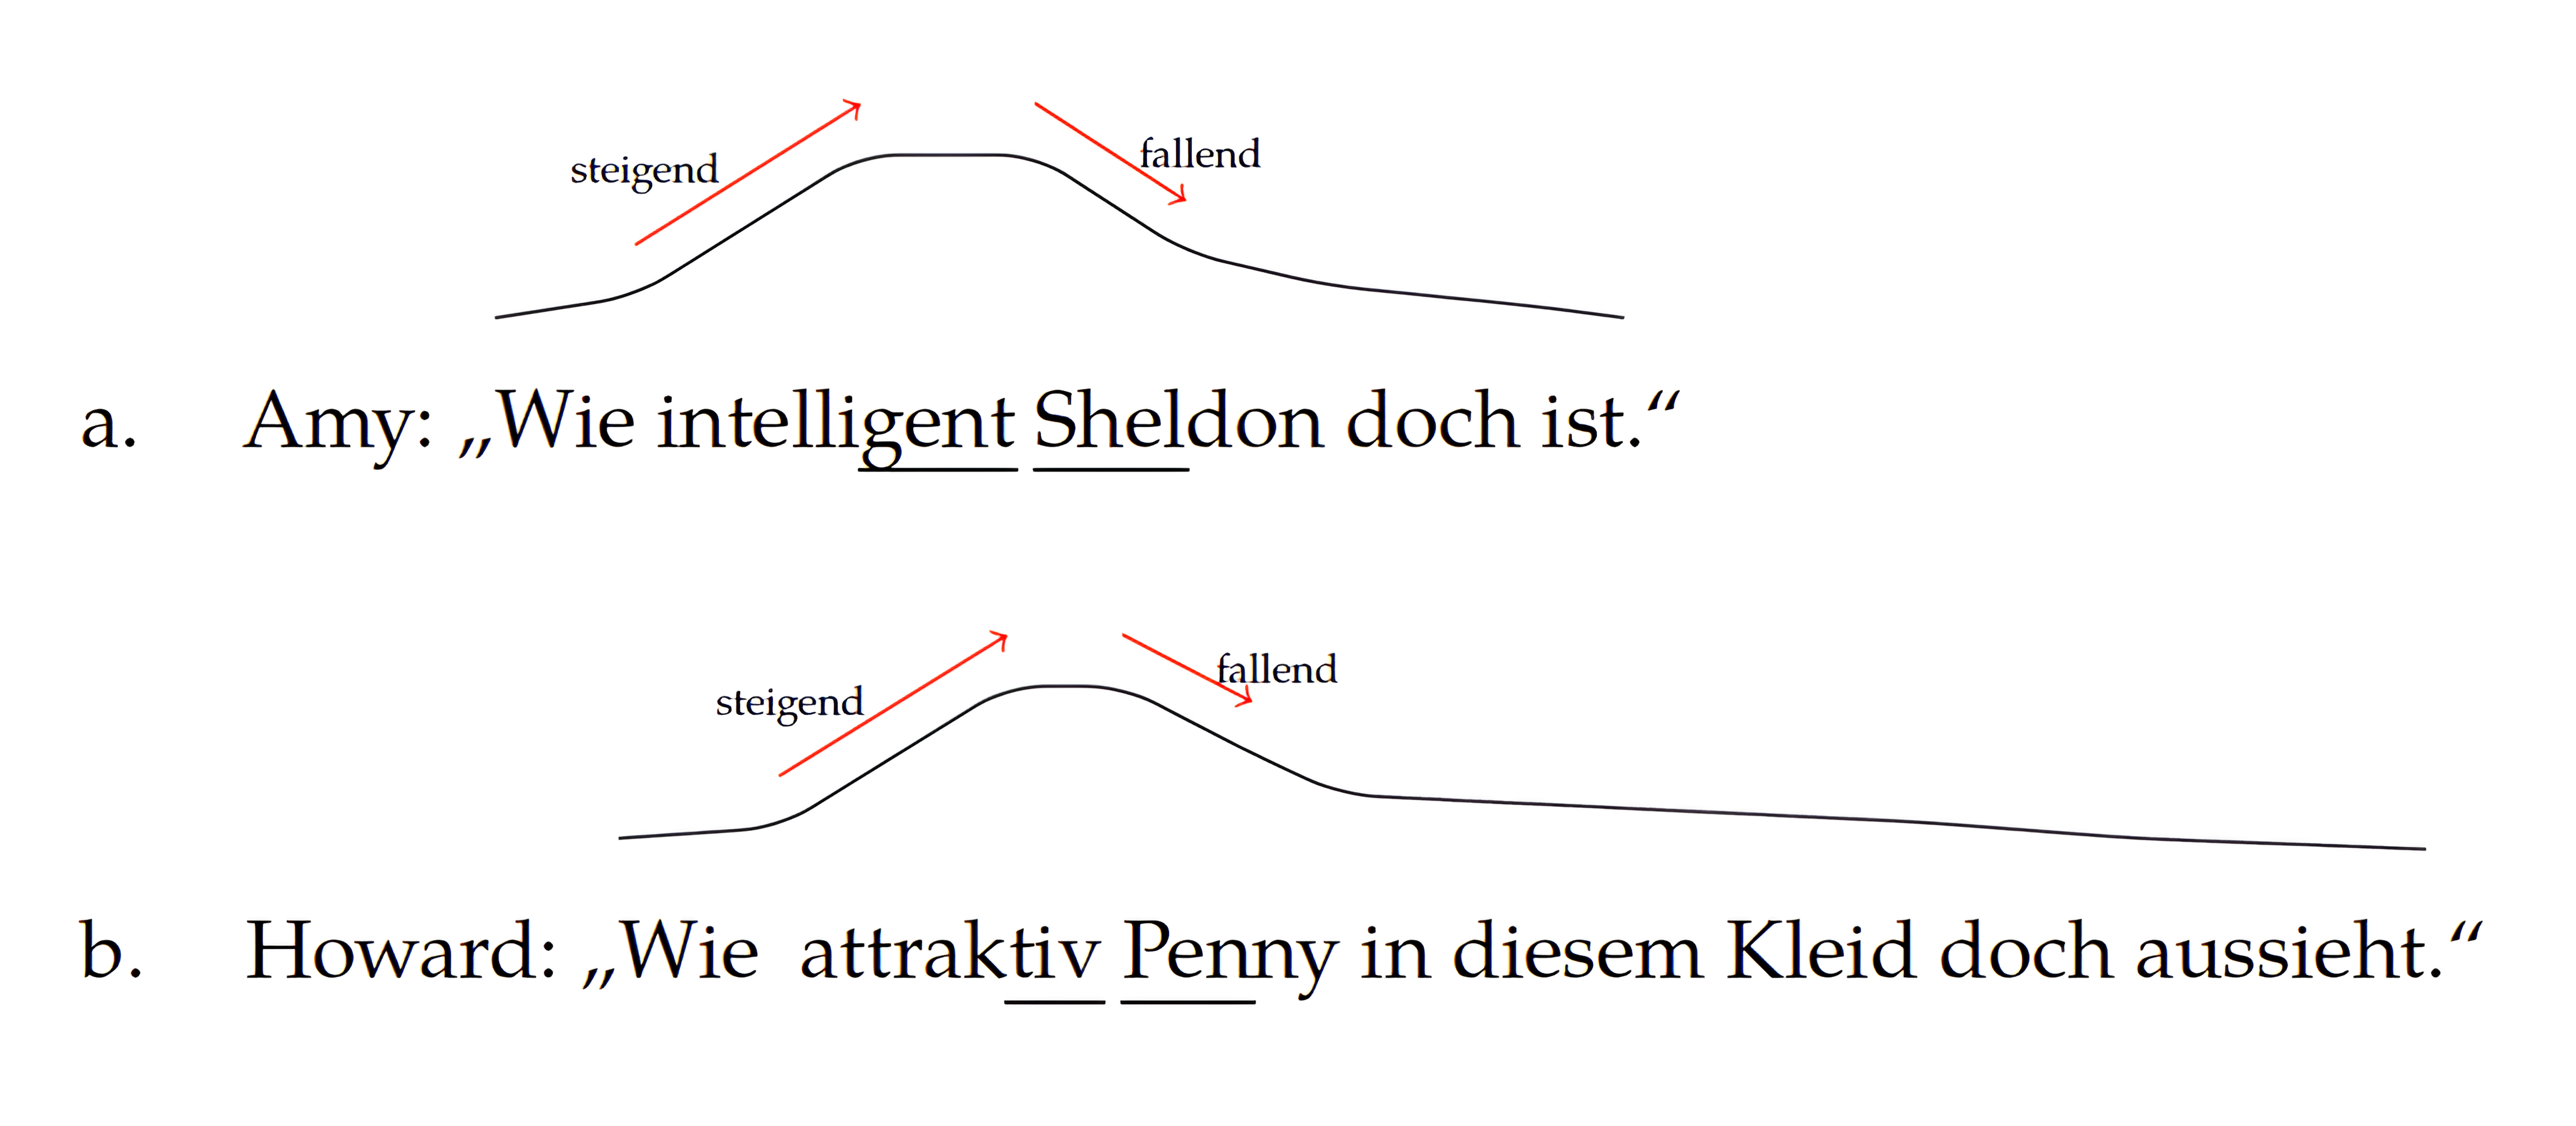
\includegraphics[width=0.9375\textwidth]{figures/Kontur3.png}%
  }
  \caption[Intonationskonturen für Exklamativsätze]
  {Intonationskonturen für die Sätze in Beispiel \REF{exklamativ}.}
  \label{Kont}
\end{figure}


\noindent Beispiel \REF{exklamativ} verdeutlicht, dass über den Exklamativsatz hinaus aus pragmatischer Sicht nichts weiter gesagt werden muss, um die Bewunderung Amys für Sheldons Intelligenz bzw. das Begehren Howards Penny gegenüber vollumfänglich und unmissverständlich zum Ausdruck zu bringen. Semantisch drücken die graduierbaren Adjektive \textit{intelligent} und \textit{attraktiv} einen überdurchschnittlich hohen Grad der im Satz beschriebenen Eigenschaft aus, der die Erwartungen des Sprechers potenziell übersteigt {\citep[vgl.][412]{Rett.2011}}. Durch die exklamative Konstruktion wird die durch den Kontext saliente Merkmalsausprägung in besonderem Maße herausgestellt, ohne dass ein Rückgriff auf eine vorherige Äußerung erforderlich ist. Ebenso wie Interjektionen haben Exklamativsätze ausschließlich expressive Bedeutung, die unabhängig von den Wahrheitsbedingungen des Satzes und deren Relevanz somit pragmatischer Natur ist (vgl. {\citealt[79]{Auer.2016}}).

\subsubsubsection{Expressive Adjektive}

Eine weitere Erscheinungsform stellen expressive Adjektive wie \textit{verdammt} oder \textit{verflucht} dar.\footnote{Das am häufigsten untersuchte expressive Adjektiv ist zweifelsohne \textit{damn}, das in der Literatur breiten Anklang gefunden und mitunter zur Diskussion von Expressivität angeregt hat (vgl. u.\,a. \citealt[]{Potts.2005, Potts.2007a, Potts.2007b}).} Diese können sowohl prädikativ als auch attributiv verwendet werden, wie die folgenden Beispiele zeigen:

 \ea  \label{ExAd1}
 \ea Penny: \glqq{}Ich finde Physik \textbf{öde}.\grqq{} \label{penn}
 \ex Bernadette: \glqq{}Dieses Kleid sieht \textbf{fantastisch} aus.\grqq{} \label{bernadette1}
  \z
 \z

  \ea  \label{ExAd10}
 \ea Kripke: \glqq{}Dieser \textbf{verdammte} Sheldon hat den Nobelpreis nicht verdient!\grqq{} \label{kripke2}
 \ex Sheldon: \glqq{}Dieser \textbf{verfluchte} Leonard hat wieder gegen die Mitbewohnervereinbarung verstoßen!\grqq{} \label{sheld}
 \z
 \z
Bei den beiden Sätzen in Beispiel \REF{ExAd1} handelt es sich der syntaktischen Form nach um Prädikative. Wenn Penny die Physik in Satz \REF{penn} als \textit{öde} bezeichnet, bezweckt sie damit keine qualitative Einordnung der wissenschaftlichen Disziplin, sondern sie möchte in erster Linie ihre persönliche Einstellung kundtun, indem sie ihr einen bestimmten (hier: niedrigen) Interessantheitsgrad zuschreibt. Ähnlich verhält es sich bei Bernadettes Äußerung in {Satz \REF{bernadette1}}: Auch hier drückt die Sprecherin ihre subjektive Bewertung aus und schreibt dem im Kontext bezeichneten Kleid (im Vergleich zu einem normal schönen Kleid) einen übermäßig hohen Ästhetikgrad zu. Während ebensolche Prädikative obligatorisch für die Bildung eines grammatischen Satzes sind und somit gemischte Bedeutungsbestandteile aufweisen, sind die attributiven Adjektive in den Sätzen \REF{kripke2} und \REF{sheld} hingegen als rein expressiv zu klassifizieren. Im Gegensatz zu ersteren leisten sie keinen Beitrag zum deskriptiven Gehalt der Äußerung und dienen daher ausschließlich der Einstellungsbekundung des Sprechers. Die attributiven Adjektive \textit{verdammte} und \textit{verfluchte} beschreiben also keine objektiven Merkmale von Sheldon oder Leonard, die als Unterscheidungskriterium zu anderen gleichnamigen Personen dienen. Stattdessen geben sie eine sprecherbezogene Charakterisierung der bezeichneten Person wieder, die grundsätzlich fakultativ ist und weggelassen werden kann, wenn der Sprecher seine persönliche Haltung zu Sheldon oder Leonard nicht ausdrücken will (vgl. \citealt[18]{Potts.2005}; {\citealt[131]{Gutzmann.2011}}).

Davon abzugrenzen sind die von \citet[]{Gutzmann.2013a} als \glqq{}functional mixed expressives\grqq{} bezeichneten attributiven Adjektive, die genauso wie die oben beschriebenen Prädikative gleichermaßen deskriptive und expressive Bedeutung tragen. Dies wird an den folgenden Sätzen illustriert:

\ea  \label{ExAd1b}
  \ea Penny: \glqq{}Ich laufe gerade von einem \textbf{beknackten} Vorsprechen zum nächsten -- ohne Erfolg.\grqq{} \label{penn1}
   \ex Amy: \glqq{}Sheldons \textbf{beschissene} Laune geht mir inzwischen schrecklich auf die Nerven.\grqq{} \label{amy1b}
 \z
 \z
Anders als bei den Adjektiven in Beispiel \REF{ExAd10} handelt es sich in \REF{ExAd1b} um Ausdrücke mit gemischten Bedeutungsanteilen: Neben der Sachverhaltsbeschreibung wird in beiden Fällen die Einstellung der Sprecherin ausgedrückt, die über den deskriptiven Gehalt der Äußerung hinausgeht. Dies erklärt {\citet[84f.]{Gutzmann.2019a}} damit, dass solche Qualitätsadjektive wie die exemplarisch in \REF{ExAd1b} herausgegriffenen gemäß ihres Ausprägungsgrades auf eine Skala abgebildet werden können: in Satz \REF{penn1} ausgehend von einem herausragenden Vorsprechen bis hin zu einem lausigen Vorsprechen, in Satz \REF{amy1b} von guter Laune bis hin zu miserabler Laune (vice versa). Ausschlaggebend für die Interpretation ist der Äußerungskontext, der die Merkmalsausprägung in die jeweils einschlägige Richtung steuert {\citep[vgl.][85]{Gutzmann.2019a}}.

Zweifelsfälle evaluativer Adjektive stellen die in der Literatur vielfach erörterten Prädikate dar, die mit individuellen Perzeptions- bzw. Geschmacksurteilen einhergehen (\glqq{}predicates of personal taste\grqq{} ({\citealt[]{Lasersohn.2005}})).

\ea  \label{ExAd2}
\ea Sheldon: \glqq{}Penny, die Spaghetti mit Würstchen sind \textbf{lecker}.\grqq{} \\
Leonard: \glqq{}Nein, sind sie nicht -- sie sind widerlich.\grqq{}
\ex Penny: \glqq{}Ich finde, dieses Nichtnewtonsche Fluid sieht \textbf{ekelhaft} aus.\grqq{} \\
Rajesh: \glqq{}Nein, gar nicht wahr. Es sieht total abgefahren aus.\grqq{}
 \z
 \z
Die Besonderheit solcher Adjektive wie die in \REF{ExAd2} aufgeführten ist, dass sie eine Eigenschaft beschreiben, die qua Semantik notwendigerweise sprecherbezogen und folglich nicht wahrheitsfunktional ist. Diese Subjektivität macht es jedoch schwierig, eine trennscharfe Grenze zwischen deskriptiver und expressiver Bedeutung zu ziehen, da es nicht möglich ist, die Aussage von Penny bzw. Sheldon als wahr oder falsch zu klassifizieren: Nur weil Sheldon die Spaghetti mit Würstchen lecker findet, heißt das nicht zwangsläufig, dass sie auch ein anderer mögen würde (vgl. die Antwort Leonards). Somit können in Abhängigkeit von Sprecher, Kontext und Perspektive verschiedene Aussagen und Qualitätsurteile zutreffen. In solchen Fällen wird der Wahrheitsgehalt der Äußerung also auf ein bestimmtes Subjekt relativiert, wobei sich der Geschmack eines Individuums von dem von anderen unterscheiden kann. Da es keinen objektiven Maßstab für solche Geschmacksurteile gibt, lässt sich bekanntlich nicht darüber streiten. Die Interpretation von Geschmacksprädikaten hänge primär davon ab, wer der kontextuelle \glqq{}Judge\grqq{} ({\citealt[665]{Lasersohn.2005}}), d.\,h. der Experiencer, ist, der oftmals, allerdings nicht notwendig dem Sprecher entspreche (vgl. \citealt[325f.]{Kaiser.2017b};; \citealt[224f.]{Kaiser.2017a}). Dadurch, dass sie die persönliche Meinung des Sprechers ausdrücken und demzufolge nicht bloß objektiv beschreibend sind, verfügen sie über Eigenschaften, die sie mit Expressiva teilen. Ob und inwiefern Geschmacksprädikate aufgrund der subjektiven Komponente tatsächlich als expressiv zu bewerten sind, wird in der Literatur kontrovers diskutiert (vgl. u.\,a. \citealt[]{Lasersohn.2005}; \citealt[]{Harris.2009}; \citealt[]{Gutzmann.2016a}).


\subsubsubsection{Expressive Nomen}

Abgesehen von expressiven Adjektiven stellen auch expressive Nomen, wie das von \citet[168]{Potts.2007b} ausführlich besprochene \textit{bastard}, eine Form von Expressivität dar. Diese kommen in der Regel in prädikativer oder appositiver Verwendung vor. Die Art des Gebrauchs bestimmt dabei den zugrunde liegenden Bedeutungstyp, wie die Beispiele \REF{ExNom} und \REF{ExNoma} illustrieren.

\ea  \label{ExNom}
\ea Amy: \glqq{}Sheldon ist ein \textbf{Genie}.\grqq{} \label{amy2}
\ex Leslie: \glqq{}Sheldon ist ein \textbf{Blödmann}.\grqq{} \label{leslie}
 \z
 \z

\ea  \label{ExNoma}
\ea Kripke: \glqq{}Dieser \textbf{Blödmann} Sheldon ist sogar verheiratet.\grqq{} \label{kripke4}
\ex Präsident Siebert: \glqq{}Dieses \textbf{Genie} Sheldon hat den Nobelpreis verdient.\grqq{} \label{siebert}
 \z
 \z
Während es sich in den Sätzen \REF{amy2} und \REF{leslie} um obligatorische expressive Nomen in prädikativer Verwendung handelt, sind die appositiv gebrauchten Nomen in den Sätzen \REF{kripke4} und \REF{siebert} optional. In Kopulakonstruktionen trägt die Bedeutung ebensolcher Nomen zur Proposition bei, weswegen sie als wahrheitsfunktional und somit deskriptiv zu klassifizieren sind. Demgegenüber weisen appositiv gebrauchte Nomen ausschließlich expressive Bedeutung auf, die keine Relevanz für den Wahrheitswert der Äußerung hat. Weil ihr Gebrauch in dieser Position fakultativ ist, können sie gleichfalls weggelassen werden, verbunden mit der Konsequenz, dass die subjektive Einstellungsbekundung des Sprechers verschwindet. Dies zeigt, dass den beiden Nomen \textit{Genie} und \textit{Blödmann} in Abhängigkeit der Verwendung unterschiedliche Bedeutungsanteile zukommen: Im Falle der prädikativen Verwendung erfolgt eine qualitative Beschreibung von Sheldon, d.\,h., Sheldon wird eine bestimmte Eigenschaft zugeschrieben (nämlich ein Genie oder ein Blödmann zu sein). Kommen die Nomen in Gestalt eines Appositivs daher, so drücken sie eine subjektive Bewertung des Sprechers aus, die ausschließlich expressiver Natur ist und nicht auf die Wahrheitsbedingungen einwirkt, wie u.\,a. \citet[270]{Gutzmann.2015a} erläutert. Eine besondere Form expressiver Nomen stellen die oftmals erörterten nationalitätsbezogenen, stereotypisierenden Beleidigungswörter wie \textit{Kartoffel} oder \textit{Kraut} (Ethnophaulismen für `Deutsche:r') (vgl. u.\,a. \citealt[2]{McCready.2010}; {\citealt[]{Croom.2013,Croom.2015}}; \citealt[20]{Gutzmann.2015a}; {\citealt[40]{Technau.2018}}) sowie emotional gefärbte Ausdrücke wie \textit{Gaul} oder \textit{Köter} mit gemischten Bedeutungstypen dar, die in Abschnitt \ref{Eigenschaften} genauer betrachtet werden.

\subsubsubsection{Modalpartikeln}

Auch Modalpartikeln wie \textit{doch} oder \textit{eben}, die häufig von polysemen Ausdrücken anderer Wortarten (z.\,B. Adverbien und Adjektiven) abgeleitet sind, werden in der Literatur als Ausprägungsform von Expressivität beschrieben. Wie {\citet[9]{Weydt.1969}} anmerkt, wurden Modalpartikeln früher häufig als funktionslose, weglassbare \glqq{}`Flick'- oder `Füllwörter'\grqq{} betrachtet, die vorwiegend in der gesprochenen {(Umgangs-)Sprache} zu finden und in der Schriftsprache zu vermeiden seien. Im Unterschied zu anderen Formen (bspw. Interjektionen) drückt der Sprecher seine Einstellung zum Geäußerten durch Modalpartikeln nicht direkt aus. So modifizieren sie nicht nur einen graduierbaren Ausdruck derselben Phrase, sondern den Satz als Ganzes {\citep[vgl.][603]{Duden.2016}}. Die Einstellungsspiegelung kann je nach verwendeter Partikel kommunikativ unterschiedlich wirken, z.\,B. permissiv oder provokativ: \textit{Komm \uline{ruhig} her} (beruhigend durch fehlenden Intensitätsgrad) vs. \textit{Komm \uline{bloß} her} (drohend aufgrund hohen Intensitätsgrades) (vgl. {\citealt[20f.]{Batinic.2015}}; {\citealt[24]{Pittner.2015}}). Daraus lässt sich schließen, dass Modalpartikeln entgegen früherer Behauptungen weder bedeutungslos noch frei austauschbar sind: \glqq{}Sie haben aber Bedeutungen. Jedoch vermitteln diese nicht Kerninformationen, sondern Zusatzinformationen\grqq{} (\citealt[89]{Weydt.1969}), die auf die subjektive Sprecherbewertung abzielen. Da sie allerdings keine eigene, mittels Wahrheitswerten beschreibbare lexikalische Bedeutung tragen und somit auch keine neuen Informationen zum deskriptiven Gehalt beisteuern,\footnote{Hiervon auszunehmen ist die von \citet[]{Zimmermann.2004} diskutierte Modalpartikel \textit{wohl}, die infolge ihrer epistemischen Interpretation durchaus relevant für die \mbox{Wahrheitsbedingungen sei}.} haben sie eine rein expressive Bedeutung und sind daher pragmatische Funktionsträger. Dies wird im Anschluss mithilfe der Modalpartikeln \textit{halt}, \textit{ja} und \textit{wohl} exemplifiziert.

\ea  \label{MoPa}
\ea Präsident Siebert: \glqq{}Sheldon ist \textbf{halt} anstrengend.\grqq{} \label{siebert2}
\ex Bernadette: \glqq{}Howard wohnt \textbf{ja} noch bei seiner Mutter.\grqq{} \label{bernadette2}
\ex Rajesh: \glqq{}Penny hat die Schauspielrolle \textbf{wohl} bekommen.\grqq{} \label{raj2}
 \z
 \z
Die Sätze im obigen Beispiel zeigen, dass die Sprechereinstellung in Abhängigkeit von der jeweils verwendeten Partikel verschieden ausgedrückt wird.\footnote{Zu erwähnen ist, dass Modalpartikeln grundsätzlich ambig sein können und deswegen stets kontextsensitiv bewertet werden müssen \citep[vgl.][603]{Duden.2016}.} Die Modalpartikel \textit{halt} in Satz \REF{siebert2} gibt an, dass Präsident Siebert die Unveränderlichkeit des Sachverhalts bekannt ist und er sich (notwendigerweise) damit abgefunden hat \citep[vgl.][10]{Abraham.1986}. Obendrein drückt Bernadette mit \textit{ja} in Satz \REF{bernadette2} aus, dass sie annimmt, der Umstand, dass Howard bei seiner Mutter wohnt, sei unkontrovers und Teil des gemeinsamen Wissenshintergrunds, den sie und der Adressat miteinander teilen (vgl. {\citealt[36f.]{Weydt.1969}}; {\citealt[19]{Abraham.1986}}). Durch die Modalpartikel \textit{wohl} in Satz \REF{raj2} erhält {Rajeshs} {Äußerung} eine epistemische Interpretation, mithilfe derer er seine bloße Vermutung hinsichtlich der Korrektheit der Sachlage mitteilt, ohne sich eindeutig darauf festlegen zu wollen \citep[vgl.][18]{Abraham.1986}.

Im Hinblick auf \textit{wohl} ist auch die sprachgeschichtliche Entwicklung interessant, die der Ausdruck auf dem Weg zur Modalpartikel durchlaufen hat. So schildert \citet[219f.]{Kip.1900}, dass sich das Adverb zunächst im Alt- und Mittelhochdeutschen\footnote{Das Althochdeutsche umfasst die Sprachstufe zwischen 750 und 1050, woran sich im Zeitraum von 1050 bis 1350 das Mittelhochdeutsche anschließt \citep[vgl.][5f.]{Nuebling.2013}.} zum Intensivierer mit der Bedeutung `völlig, gewiss, sehr' entwickelt hat. Diese Gradbedeutung hat sich mit der Zeit jedoch abgeschwächt, sodass die Partikel in neuerer Sprachperiode nur noch modal zum Ausdruck von Behauptungen oder Mutmaßungen gebraucht wird.

\subsubsubsection{Pronomen}

Ein weiterer, wenn auch weniger evidenter Fall von Expressivität liegt bei Ausdrücken mit sozialer Bedeutung wie Nähe- und Distanzformen vor, die in verschiedenen Sprachen zu finden sind (bspw. im Deutschen oder Französischen). Obwohl sie weder Einstellungsbekundungen noch emotionale Zustände des Sprechers wiedergeben, sind sie dennoch mit einer rein expressiven Funktion versehen, die nicht auf deskriptiver Ebene {verankert ist}.

\ea  \label{NäDi}
\ea Präsident Siebert: \glqq{}Ich rufe \textbf{Sie} an, Sheldon.\grqq{} \label{siebert3}
\ex Bernadette: \glqq{}Hast \textbf{du} Penny gesehen, Leonard?\grqq{} \label{bernadette3}
 \z
 \z
Anhand der Sätze in Beispiel \REF{NäDi} lässt sich verdeutlichen, dass es keinen Unterschied in der referentiellen Bedeutung der förmlichen Anrede \textit{Sie} und der formlosen Balanceform \textit{du} gibt. Nach \citet[33]{Loebner.2002} bedeutet dies, dass sich beide Anredeformen insofern nicht voneinander unterscheiden, als sie gleichermaßen auf einen bestimmten Adressaten Bezug nehmen. Somit referieren sowohl Präsident Siebert mit der Verwendung der Distanzform \textit{Sie} in Satz \REF{siebert3} als auch Bernadette mit der Näheform \textit{du} in Satz \REF{bernadette3} auf eine bestimmte Person, nämlich Sheldon und Leonard. Darüber hinaus geht \textit{Sie} zusätzlich mit einem sozialen Bedeutungsanteil einher, der der informellen Form gänzlich fehlt \citep[vgl.][33]{Loebner.2002}. Dieser nicht-propositionale Bedeutungsbestandteil ermöglicht es dem Sprecher, per Konvention eine interpersonelle Distanz zum Gegenüber anzuzeigen, die in der Regel auf Unbekanntheit, Höflichkeitsstreben oder eine soziale Hierarchie zurückgeht \citep[vgl.][18]{Pafel.2016}. Infolgedessen ist anzunehmen, dass der Unterschied zwischen dem formlosen \textit{du} und dem förmlichen \textit{Sie} durch einen Kontrast in der sozial-expressiven Komponente bedingt ist. Nach {\citet[26]{Gutzmann.2019a}} handelt es sich bei solchen Pronomen um gemischte Expressiva, die zugleich deskriptive wie expressive Bedeutungsbestandteile aufweisen. Seiner Notation folgend befindet sich auf der deskriptiven Ebene der Adressat, der den Referenten des jeweiligen Kontexts darstellt. Auf der expressiven Ebene sieht er die für die Gebrauchsbedingungen relevante Unterscheidung zwischen der formellen und informellen Form verankert: \glqq{}[C]hoosing the wrong pronoun can never make an otherwise true sentence false, but it may result in a high degree of social infelicity.\grqq{} (\citealt[26]{Gutzmann.2019a}). Fehlt diese expressive Zusatzkomponente, so kann der Ausdruck im Kontext folglich als unpassend oder gar unhöflich aufgefasst werden: Auch wenn Präsident Siebert Sheldon gegenüber im Prinzip ebenso das weniger formelle \textit{du} verwenden könnte, würde es aufgrund der sozialen  Hierarchie der Arbeitgeber-Arbeitnehmer-Beziehung möglicherweise als unangemessen wahrgenommen. Genauso inadäquat kann ihr Vorhandensein in informellen Kontexten sein. So riefe es bei Leonard vermutlich starke Irritation hervor, wenn ihn Bernadette trotz jahrelanger Freundschaft plötzlich siezte, da eine solche förmliche Ausdrucksweise in dem Fall nicht angebracht ist.

\subsubsubsection{Dativus ethicus}

Daneben sind auch ethische Dative im Allgemeinen eng mit dem Begriff der Expressivität verbunden, die bspw. in verschiedenen germanischen, romanischen oder slawischen Sprachen vorkommen und nach \citet[61]{Wegener.1989} als \glqq{}Ausdruck familiärer Vertrautheit\grqq{} gelten. Dies zeigt \citet[26f.]{Gutzmann.2019a} am Beispiel des Englischen und Deutschen wie folgt:

\ea  \label{EtDat}
\ea I want \textbf{me} an iPod. \hfill  \citep[][175]{Horn.2008} \label{iPod}
\ex Dass du \textbf{mir} ja nicht zu spät kommst. \hfill  \citep[][5]{Lambert.2007} \label{spät}
 \z
 \z
In beiden Sätzen \REF{iPod} und \REF{spät} drückt der freie Dativ eine emotionale Beteiligung des Sprechers in Form einer Bitte oder einer Warnung aus, die nicht Teil des deskriptiven Gehalts der Äußerung ist. Dementsprechend hat er keinerlei Auswirkungen auf die Wahrheitsbedingungen des Satzes. Stattdessen ist der ethische Dativ vielmehr als zusätzliche Bedeutungskomponente zu klassifizieren, mit deren Hilfe der Sprecher seine persönliche Involviertheit in den Sachverhalt anzeigen kann \citep[vgl.][27]{Gutzmann.2019a}. \glqq{}[D]ie Quelle der ausgedrückten Einstellung\grqq{} (\citealt[68]{Wegener.1989}) liege dabei stets beim Sprecher, was im obigen Beispiel durch das Reflexivpronomen der 1. Person \textit{mir} (bzw. \textit{me}) ausgedrückt wird. Da das jeweilige Pronomen keinen Einfluss auf den deskriptiven Gehalt nimmt, kann es ohne Bedeutungsänderung eliminiert werden. Die unmittelbare Folge des Auslassens ist allerdings, dass die expressive Bedeutungskomponente, d.\,h. die ausgedrückte Sprecherbeteiligung, verschwindet und nur der deskriptive Gehalt der Äußerung bestehen bleibt. Laut \citet[69]{Wegener.1989} dient der ethische Dativ somit vordergründig dazu, \glqq{}auf das emotiv-affektive Involviertsein des Sprechers zu verweisen bzw. ein solches Involviertsein beim Hörer {zu unterstellen\grqq{}}.

\subsubsubsection{Expressive Vokative}

Auch \glqq{}expressive Vokative\grqq{} (\citealt[172]{Gutzmann.2019a}) werden in der theoretischen Literatur als eine Ausprägung von Expressivität behandelt. Während klassische Vokative normalerweise durch Substantive oder Eigennamen repräsentiert und nach \citet[787]{Zwicky.1974} aus pragmatischer Sicht hauptsächlich zur Aufmerksamkeitssteuerung verwendet werden, bestehen expressive Vokative aus einem Personalpronomen und einem (expressiven) Nomen. Dies macht \citet[188]{Gutzmann.2019a} an den folgenden Beispielen deutlich:

\ea  \label{ExVo}
\ea \textbf{You idiot!} \label{idiot}
\ex \textbf{You bastard!} \label{bastard0}
 \z
 \z

\ea  \label{ExVo2}
\ea \textbf{You linguist!} \label{linguist}
\ex \textbf{You philosopher!} \label{philosopher}
 \z
 \z
Die beiden Sätze in Beispiel \REF{ExVo} beinhalten mit \textit{idiot} und \textit{bastard} expressive Nomen, die qua Semantik eine bewertende, in diesem Fall negative Sprechereinstellung ausdrücken. Dagegen handelt es sich bei \textit{linguist} und \textit{philosopher} {in Beispiel \REF{ExVo2}} um neutrale Nomen, die über ihre lexikalische Bedeutung hinaus keine zusätzliche evaluative Bedeutungskomponente aufweisen. Dennoch erhalten die Ausdrücke durch solche Vokativkonstruktionen eine expressive Interpretation, die als eine persönliche Bewertung des Sprechers aufzufassen ist. Der Unterschied zwischen dem ersten und zweiten Satzpaar liegt im Wesentlichen darin, dass die Sprechereinstellung bei ersterem aufgrund der klar wahrnehmbaren evaluativen Semantik der Ausdrücke erheblich stärker kommuniziert wird. Bei letzterem wird die Sprechereinstellung hingegen erst durch die Konstruktion ausgedrückt, wodurch sie als vergleichsweise moderater und weniger offensiv wahrgenommen wird (vgl. {\citealt[212]{dAvis.2013}}; {\citealt[188f.]{Gutzmann.2019a}}). In Abhängigkeit des Kontexts können ebensolche eigentlich neutralen Nomen wie \textit{linguist} und \textit{philosopher} in Vokativkonstruktionen gleichermaßen positiv wie auch negativ interpretiert werden, d.\,h. als Ausdruck der Bewunderung oder als Beschimpfung. Gegenläufig zu den klassischen Vokativen haben expressive Vokative keine aufmerksamkeitssteuernde Funktion. Aus diesem Grund ist es mit ihnen nicht möglich, zwischen einer Masse an Referenten und Einzelpersonen zu differenzieren, weswegen sie \citet[]{dAvis.2013} als \glqq{}pseudo-vocative constructions\grqq{} bezeichnen {\citep[vgl.][189]{Gutzmann.2019a}}.

\subsubsection{Eigenschaften von Expressivität}  \label{Eigenschaften}
Gegenstand dieses Abschnitts sind die Merkmale von sprachlicher Expressivität sowie die Kriterien, die in der theoretischen Literatur für die Unterscheidung zwischen deskriptivem und expressivem Gehalt angeführt werden. Aus der Akzeptanz zweier Bedeutungstypen und der Definition von Expressivität ex negativo ergeben sich mehrere Streitfragen: Worin besteht der semantische Unterschied zwischen deskriptiver und expressiver Bedeutung? Wie lassen sich die Bedeutungstypen voneinander abgrenzen? Und was sind die Besonderheiten expressiver Bedeutung? 
Einige Autor:innen, (z.\,B. {\citealt[]{Cruse.1986}}, {\citealt[]{Kaplan.1997}} oder {\citealt[]{Potts.2005, Potts.2007a}}), haben sich aus formal-semantischer Perspektive mit den Eigenschaften von Expressivität auseinandergesetzt. Als wegbereitend gelten auf diesem Gebiet vor allem die Ausführungen von {\citet[]{Potts.2007a}}. Er baut im Kern auf den in Abschnitt {\REF{Arbeitsdefinition}} geschilderten Ansätzen auf und entwickelt durch die Annahme von zwei verschiedenen Dimensionen einen neuen Zugang zu sprachlicher Bedeutung. In diesem Kontext erarbeitet er sechs Kriterien, die es ermöglichen, expressive Bedeutung als solche zu identifizieren und von deskriptiver zu separieren. Diese Kriterien werden im Anschluss präsentiert.

Das erste Kriterium nennt \citet[167ff.]{Potts.2007a} \textit{Independence} (`Unabhängigkeit'). Nach diesem stellen die beiden Bedeutungstypen zwei separate, voneinander unabhängige Dimensionen dar. Da die expressive Ebene nicht an die deskriptive Ebene gebunden sei, können Sprecher die in einer Äußerung enthaltenen expressiven Bedeutungsbestandteile beliebig verändern oder weglassen, ohne dass dies auf den deskriptiven Gehalt einwirke. Dieses {Prinzip} lässt sich im Sinne von \citet[168]{Potts.2007a} und \citet[9]{dAvis.2019b} wie folgt illustrieren:

\ea  Dieser \,\textbf{bescheuerte}\,/\,\textbf{dämliche} Sheldon ist ein Nerd. \label{sheldon}
\ea deskriptiv: Sheldon ist ein Nerd.
\ex expressiv: Der Sprecher mag Sheldon nicht.
 \z
 \z

Beispiel \REF{sheldon} demonstriert, dass eine Variation derjenigen Ausdrücke, die expressive Bedeutung aufweisen (d.\,h. \textit{bescheuerte} oder \textit{dämliche}) keine Veränderung des deskriptiven Gehalts nach sich zieht: Er bleibt von der Änderung auf expressiver Ebene unangetastet. Gleichsam kann das expressive Adjektiv eliminiert werden, ohne dass die Proposition davon betroffen ist. Dies zeigt, dass es sich bei deskriptiver und expressiver Bedeutung um zwei eigenständige, voneinander getrennte Ebenen handelt, deren Einzelbedeutungen zur Gesamtbedeutung des Satzes verknüpft werden. Aufgrund ihrer Expressivität haben die verwendeten attributiven Adjektive keinen Einfluss auf die Wahrheit oder Falschheit des Satzes. Stattdessen drücken sie die persönliche Einstellung des Sprechers aus, bei der statt Wahrheitsbedingungen die oben beschriebenen Gebrauchsbedingungen Anwendung finden. Gemäß der in {\citet[5]{Gutzmann.2013a}} vorgeschlagenen Notation lassen sich die beiden semantischen Dimensionen von Beispiel \REF{sheldon} folgendermaßen schematisch darstellen:\footnote{Zu beachten ist, dass die Konklusion der deskriptiven Bedeutung des Satzes entspricht, während die Prämisse die expressive Bedeutung in Form einer Zusatzebene repräsentiert.} \medskip

Dieser bescheuerte Sheldon ist ein Nerd = \begin{large} $\frac{\text{Der Sprecher mag Sheldon nicht}}{\text{Sheldon ist ein Nerd}}$ \end{large} \medskip

\citet[8]{Kaplan.1997} zufolge kann expressive Bedeutung weder negiert noch konditionalisiert werden: Wenn der Adressat dem Sprecher beim obigen Satz widerspricht, weist er zwar das Zutreffen des bezeichneten Sachverhalts zurück, nicht aber den zusätzlichen expressiven Gehalt. Dies sei ein weiterer Indikator für die Eigenständigkeit der Bedeutungsdimensionen.

Dessen ungeachtet weicht \citet[168]{Potts.2007a} das Unabhängigkeitskriterium auf und ergänzt, dass die beiden Bedeutungstypen allerdings nicht völlig unabhängig voneinander sind, greifen expressive Ausdrücke doch insofern auf die deskriptive Ebene zu, als sie darauf ihr Argument finden. So benötigt das aus semantischer Sicht als Prädikat zu betrachtende \textit{bescheuerte} oder \textit{dämliche} ein Argument, auf dem es operiert. Ebendieses findet es im deskriptiven Gehalt, genauer gesagt im Eigennamen, d.\,h. in \textit{Sheldon}, wie \citet[9]{dAvis.2019b} erläutern. Inwiefern die Bedeutungstypen einander noch bedingen, wird beim vierten Kriterium wieder aufgegriffen.

Das zweite Kriterium bezeichnet \citet[169ff.]{Potts.2007a} als \textit{Nondisplaceability} (`Nicht-Verschiebbarkeit'). Dieses resultiert aus dem deiktischen Verhalten von Expressiva, demgemäß sich expressive Bedeutung unmittelbar auf die Parameter der Äußerungssituation, d.\,h. Sprecher, Ort und Zeit etc., bezieht: \glqq{}Expressives cannot (outside of direct quotation) be used to report on past events, attitudes, or emotions, nor can they express mere possibilities, conjectures, or suppositions.\grqq{} ({\citealt[169]{Potts.2007a}}). Diese Beobachtung kongruiert mit dem von {\citet[8]{Kaplan.1997}} beschriebenen Projektionsverhalten. In der Folge vergleicht {\citet[272]{Cruse.1986}} die unmittelbare Wirkung von expressiven Ausdrücken bspw. mit Gesichtsausdrücken wie Lächeln oder Stirnrunzeln sowie anderen sprecherorientierten Gesten, die ebenfalls nur zum Zeitpunkt der Äußerung angebracht sind. Die Idee dahinter wird in Anlehnung an die von {\citet[10]{dAvis.2019b}} formulierten Beispielsätze verdeutlicht.\footnote{Die Raute (\#) symbolisiert hier und im weiteren Verlauf, dass der Satz bzw. eine solche Fortsetzung pragmatisch nicht im intendierten Sinne möglich ist.}

\ea   \label{sheldon2}
\ea[]{Dieser Klugscheißer Sheldon ist nicht überheblich. (\#Ich kann ihn gut leiden.) \label{negation1}}
\ex[]{Glücklicherweise ist es nicht wahr, dass dieser Klugscheißer Sheldon überheblich ist. (\#Ich kann ihn gut leiden.) \label{negation2}}
\ex[\#]{Wenn dieser Klugscheißer Sheldon ein netter Mensch ist, sollte er aufgrund seiner Überheblichkeit keine Frau finden. \label{konditional}}
\ex[]{Es ist möglich, dass sich dieser Klugscheißer Sheldon wieder überheblich benehmen wird. (\#Andererseits ist er vielleicht gar kein Klugscheißer.) \label{moeglichkeit}}
\ex[]{Dieser Klugscheißer Sheldon hat sich gestern überheblich benommen. (\#Aber heute ist er kein Klugscheißer, weil er sich normal benimmt.) \label{tempus}}
 \z
 \z

Nach Erklärung von {\citet[10]{dAvis.2019b}} werden die mit einer Raute ausgestatteten Interpretationen aus verschiedenen Gründen blockiert: Während sich die Negation in \REF{negation1} und \REF{negation2} nicht auf die persönliche Einstellung des Sprechers gegenüber Sheldon bezieht, sondern alleine die ihm zugeschriebene Charaktereigenschaft und somit den deskriptiven Gehalt negiert, wird {Satz \REF{konditional}} dadurch verhindert, dass das expressive Nomen \textit{Klugscheißer} nicht konditionalisiert werden kann. Ebenso wenig kann es von einem Möglichkeitsoperator erfasst werden, wodurch eine Interpretation wie die in \REF{moeglichkeit} ausgeschlossen ist. Zudem kann der Ausdruck in {Satz \REF{tempus}} nicht temporal modifiziert werden \citep[vgl.][10]{dAvis.2019b}. Daran ist zu erkennen, dass die Einstellungsbekundung des Sprechers durch die Verwendung des expressiven Nomens \textit{Klugscheißer} in allen Fällen erhalten bleibt und es nicht möglich ist, diese z.\,B. durch einen beschwichtigenden Zusatz aufzuheben. In diesem Kontext verweist \citet[15]{Gutzmann.2019a} auf die Ähnlichkeit zwischen expressiver Bedeutung und Präsuppositionen, projizieren doch beide gleichermaßen auf die Äußerung als Ganzes.

Das dritte Kriterium, das \citet[173ff.]{Potts.2007a} definiert, nennt sich \textit{Perspective dependence} (`Perspektivenabhängigkeit'). Dieses besagt, dass expressive Bedeutung grundsätzlich subjektive Einstellungen, Evaluationen und Emotionen ausdrückt, die sich auf eine bestimmte Perspektive beziehen. Dies sei im Regelfall der Sprecher, der als Experiencer einen Sachverhalt von seinem Standpunkt aus beurteile und seine Haltung entsprechend zum Ausdruck bringe. Eine Ausnahme stelle jedoch Redewiedergabe dar, bei der ein Perspektivenwechsel erfolgen könne, der dazu führe, dass eine andere, im Kontext saliente Person der Einstellungsträger ist \citep[vgl.][175]{Potts.2007a}. Dies zeigt das in der Literatur oft herangezogene Beispiel von {\citet[6]{Kratzer.1999}}:

\ea  My father screamed that he would never allow \uline{me} to marry \uline{that bastard Webster}. \label{bastard}
\z

In \REF{bastard} kommt aufgrund des darin enthaltenen Verbum dicendi keine andere Interpretation infrage, als dass der expressive Bedeutungsanteil dem Wortlaut des Vaters entspricht. Die Einstellungsspiegelung erfolgt also nicht in der Äußerungssituation, sondern zu einem vorangegangenen Zeitpunkt, auf den hier Bezug genommen wird \citep[vgl.][6]{Kratzer.1999}. Dass der Vater in diesem Fall der Einstellungsträger ist, hat nach \citet[11]{dAvis.2019b} neben dem erwähnten Verb des Sagens auch psychische Realität: So beabsichtige der Sprecher wohl kaum jemanden zu heiraten, der seiner Ansicht nach ein schlechter Mensch ist. Ergänzend demonstrieren sie, dass es durch eine Variation des Kontexts möglich ist, die verbalisierte Einstellung nicht dem Subjekt des übergeordneten Satzes, sondern dem Sprecher zuzuschreiben:

\ea  Mein Vater sagte, dass er es mir nie erlauben würde, dieses Arschloch Webster umzubringen.
\z

\citet[173]{Potts.2007a} erklärt den Perspektivenwechsel mit dem auf {\citet[]{Lasersohn.2005}} zurückgehenden kontextuellen \glqq{}Judge\grqq{}, d.\,h. dem Richter, der in einer Situation ein Urteil fälle und für gewöhnlich dem Sprecher entspreche. In Abhängigkeit des Kontexts bestehe die Möglichkeit, dass die Richterrolle von jemand anderem als dem Sprecher eingenommen werde. Dies ist abgesehen vom obigen Beispiel \REF{bastard} u.\,a. bei den in der Literatur vielfach diskutierten Geschmacksprädikaten festzustellen (vgl. bspw. {\citealt[]{Lasersohn.2005}}; \citealt[]{Harris.2009}; \citealt[]{Gutzmann.2016a}; {\citealt[]{Kaiser.2017b, Kaiser.2017a}}).

Das vierte Kriterium, das \citet[176ff.]{Potts.2007a} anführt, nennt sich \textit{Descriptive ineffability} (`Nicht-Beschreibbarkeit'). Dahinter steckt die bereits von {\citet[156]{Hayner.1956}} thematisierte Beobachtung, dass sich die Bedeutung von expressiven Ausdrücken nicht oder nicht hinreichend deskriptiv umschreiben lässt. Aufgrund des Umstands, dass nicht-expressive, assertive Paraphrasen nicht die gewünschte Ausdrucksstärke in sich tragen, seien sie für den Sprecher in der Äußerungssituation wenig zufriedenstellend. Laut \citet[12]{dAvis.2019b} fällt es Sprechern ohnehin schwer, expressive Bedeutungsbestandteile deskriptiv zu paraphrasieren: Versuche man bspw., einen expressiven Ausdruck wie \textit{Klugscheißer} in ein deskriptives Äquivalent zu überführen, so gehe die für Expressiva charakteristische Zusatzkomponente, die Einstellungsspiegelung also, verloren. So bedeute \glqq{}[d]ie Verwendung von \textit{Drecksack} in Bezug auf eine bestimmte Person \textelp{} nicht einfach, dass diese Person ein schlechter Mensch ist.\grqq{} ({\citealt[12]{dAvis.2019b}}). Stattdessen werde zusätzlich zum deskriptiven Gehalt ebenso die evaluative, in dem Fall negative Einstellung des Sprechers mit kommuniziert, die der deskriptiven Paraphrasierung gänzlich fehle. Aus diesem Grund lässt sich die Bedeutung eines expressiven Ausdrucks nach Auffassung von {\citet[10]{Kaplan.1997}} am ehesten durch seine korrekte Verwendung im Kontext beschreiben.

Auch Potts' (2007: 179ff.) fünftes Kriterium, \textit{Immediacy} (`{Unmittelbarkeit}'), wurde schon von \citet[151]{Hayner.1956} und \citet[285]{Cruse.1986} erkannt. Nach diesem verhalten sich expressive Ausdrücke infolge ihrer zielgerichteten, kraftvollen Natur wie performative Sprechakte\footnote{Genau wie Expressiva unterliegen auch Performativa nicht den Wahrheitsbedingungen, sondern vielmehr den Glückens- bzw. Angemessenheitsbedingungen
der fraglichen Situation (vgl. u.\,a. \citealt[75f.]{Austin.1972};; \citealt[176f.]{Chierchia.1990}).} und müssen bloß geäußert werden, um den intendierten Effekt zu erlangen: \glqq{}Like {performatives}, the act of uttering an expressive morpheme is sufficient for conveying its content. \textelp{} [T]he act of uttering an expressive \textit{is} the emotive performance.\grqq{} ({\citealt[180]{Potts.2007a}}). Dies lässt sich angelehnt an {\citet[12]{dAvis.2019b}} unter Zuhilfenahme des obigen {Beispiels \REF{tempus} aufzeigen}:

\ea  Dieser Klugscheißer Sheldon hat sich gestern überheblich benommen. (\#Aber heute ist er kein Klugscheißer, weil er sich normal benimmt.)
\z

Die Äußerung des expressiven Ausdrucks \textit{Klugscheißer} im genannten Beispiel bewirkt eine Veränderung des Kontexts, in deren Folge es für den Sprecher nicht mehr möglich ist, die damit einhergehende negative Einstellung {zurückzunehmen} oder zu relativieren. Mit anderen Worten: \glqq{}Das, was ein Sprecher damit ausdrücken will, ist im Diskurs nicht verhandelbar.\grqq{} (\citealt[12]{dAvis.2019b}). Dies lässt sich auch mittels Frage und Negation überprüfen, wie ein von \citet[31]{Gutzmann.2015a} übernommenes Beispiel illustriert:

\ea   Descartes was not a Kraut. \#But I like Germans. \label{gutzi} \\
	A: Was Descartes a Kraut? \\
    B: \#No, Germans are nice.
\z

Wie zuvor kann die bereits geäußerte negative Einstellung auch in dem \REF{gutzi} aufgeführten Beispiel nicht neutralisiert werden. Dies erklärt {\citet[31]{Gutzmann.2015a}} damit, dass Frage und Negation ausschließlich auf die wahrheitsfunktionale Ebene einwirken. Die expressive, gebrauchskonditionale Ebene bleibe davon jedoch unberührt, wie er anhand der beiden voneinander unabhängigen Bedeutungsdimensionen folgendermaßen präzisiert: \medskip

Descartes was not a Kraut. = \begin{large} $\frac{\text{Kraut}}{\text{$\neg$(Descartes was a German)}}$ \end{large} \medskip

Was Descartes a Kraut? = \begin{large} $\frac{\text{Kraut}}{\text{?(Descartes was a German)}}$ \end{large} \medskip

\noindent \citet[12]{dAvis.2019b} ergänzen weiterhin, dass die Wahrheit der kommunizierten Sprechereinstellung vom Adressaten nicht angezweifelt werden kann, wie Beispiel \REF{pups} demonstriert.

\ea  \label{pups}
\ea Howard: \glqq{}Penny hat Leonard bezüglich ihres College-Abschlusses angelogen.\grqq{} \label{penny}
\ex	Rajesh: \glqq{}Nein, das ist nicht wahr.\grqq{} ($\rightarrow$ Sie hat ihn nicht angelogen.) \label{penny1}
\ex Rajesh: \glqq{}\#Nein, das hast du jetzt nicht assertiert.\grqq{} ($\nrightarrow$ Sie hat ihn nicht angelogen.)\label{penny2}
 \z
 \z

In Satz \REF{penny1} stellt Rajesh durch die Negation \textit{nicht} den Wahrheitsgehalt von Howards Äußerung infrage. Dagegen kann er in Satz \REF{penny2} Howards Sprechakt allerdings nicht als solchen hinterfragen, weswegen eine solche Aussage nicht möglich ist \citep[vgl.][12]{dAvis.2019b}. {\citet[152]{Zifonun.1997}} zufolge können verbalisierte Expressiva lediglich dann angezweifelt werden, wenn man Bedenken in Bezug auf die Aufrichtigkeit des Sprechers hat. Da es sich dabei nämlich um subjektive Gemütszustände handele, sei ein Irrtum des Sprechers bei seiner Äußerung grundsätzlich ausgeschlossen.

 Schließlich gibt \citet[182ff.]{Potts.2007a} mit \textit{Repeatability} (`Wiederholbarkeit') ein sechstes Kriterium an, nach dem Ausdrücke mit expressiver Bedeutung beliebig oft iteriert werden können: Statt wie im Falle von {deskriptiven} Ausdrücken redundant zu sein, münde die Wiederholung expressiver {Ausdrücke} in einer Verstärkung der Aussage. Die Idee dahinter verdeutlicht {\citet[182]{Potts.2007a}} wie folgt:
 
\ea   \label{damn}
\ea Damn, I left my keys in the car.
\ex Damn, I left my damn keys in the car.
\ex Damn, I left my damn keys in the damn car.
 \z
 \z
Während die Einfügung mehrerer (und auch identischer) expressiver Ausdrücke wie \textit{damn} in Beispiel \REF{damn} ohne Redundanz möglich ist und die Verärgerung des Sprechers hinsichtlich des bezeichneten Sachverhalts maximal hervorhebt, entziehen sich deskriptive Ausdrücke oder Paraphrasen hingegen dieser Eigenschaft, wie \citet[182]{Potts.2007a} ferner hinzufügt:

\ea[\#]{I'm angry! I forgot my keys. I'm angry! They are in the car. I'm angry!}
\z

In diesem Zusammenhang bringt \citet[182]{Potts.2007a} die bspw. für das Japanische oder Koreanische typischen Honorifika\footnote{Bei Honorifika handelt es sich \citet[381]{Shibatani.2009} zufolge um \glqq{}special linguistic forms that are used to signify deference toward the nominal referent or the addressee.\grqq{} Diese auf dem sozialen Status basierende Form der Ehrerbietung können Sprecher sprachlich z.\,B. in Form von Titeln, Pronomen oder Nomen ausdrücken.} zur Sprache, die soziale Bedeutung tragen und in der gesellschaftlichen Hierarchie dazu dienen, Respekt auszudrücken. Auch bei diesen sei die Quantität entscheidend für den korrekten Gebrauch: Bei zu wenigen Honorifika laufe der Sprecher Gefahr, unhöflich zu erscheinen, wohingegen zu viele vom Adressaten als Sarkasmus oder Ironie interpretiert werden können (vgl. auch {\citealt[13]{dAvis.2019b}}).

Trotz der breiten Anerkennung, die \citet[]{Potts.2007a} für seinen Kriterienkatalog erhalten hat, gibt es dennoch Autor:innen, die seine Heuristik infrage stellen. So argumentiert bspw. \citet[209f.]{Geurts.2007}, dass die von {\citet[]{Potts.2007a}} vorgenommene Dichotomie zwischen deskriptiver und expressiver Bedeutung zu strikt sei, während er manchen Kriterien sogar die Gültigkeit abspricht. Das erste Merkmal, das \citet[210]{Geurts.2007} anficht, ist das der Nicht-Beschreibbarkeit: Diese sei keine Eigenart von Expressiva, sondern treffe auf eine Vielzahl von sprachlichen Ausdrücken zu. So seien sowohl zahlreiche Funktions- wie auch Inhaltswörter (z.\,B. \textit{the}, \textit{because} oder \textit{green}) nur schwerlich treffend zu paraphrasieren. In der Folge moniert er, dass sich dieses Kriterium kaum dazu eigne, zwischen deskriptivem und expressivem Gehalt zu unterscheiden \citep[vgl.][210]{Geurts.2007}. Darüber hinaus übt er Kritik an der Art und Weise, wie sich expressive Bedeutung bei \citet[]{Potts.2007a} aus einer Kombination einzelner Bestandteile ergibt: Analysiere man \textit{really fucking brilliant}, wie von \citet[187]{Potts.2007a} vorgeschlagen, als eine Kombination aus $(\lsem$really$\rsem$) und ($\lsem$fucking brilliant$\rsem$), wobei \textit{fucking} syntaktisch und semantisch als \textit{sehr} zu interpretieren sei, können die beiden Bedeutungsdimensionen nicht als separate Bestandteile behandelt werden. Dies stehe jedoch wiederum in direktem Kontrast zu dem von {\citet[167ff.]{Potts.2007a}} postulierten Unabhängigkeitskriterium {\citep[vgl.][211]{Geurts.2007}}. Ein weiteres Merkmal, das {\citet[211f.]{Geurts.2007}} angreift, ist das Kriterium der Nicht-Verschiebbarkeit, nach dem sich expressive Bedeutung nicht auf Vergangenes, Emotionen oder Annahmen beziehen könne. In diesem Kontext führt er einige Gegenbeispiele an, in denen es entgegen der Behauptungen von \citet[]{Potts.2007a} doch möglich ist, dass der expressive Ausdruck bspw. im Skopus eines Möglichkeitsoperators steht, wie er u.\,a. mithilfe des anschließenden Satzes exemplifiziert:
   
\ea  Perhaps it’s the codeine laced cough syrup I’ve been taking for a few days now or maybe these lines are fucking brilliant!
\z

Vor diesem Hintergrund beruft sich \citet[212]{Geurts.2007} ebenso auf den folgenden Beispielsatz nach \citet[171]{Potts.2007a}:

\ea  Whenever I pour wine, the damn bottle drips.  \label{wine}
\z

Laut \citet[171]{Potts.2007a} lässt sich aus Beispiel \REF{wine} ableiten, dass der Sprecher zum Zeitpunkt der Äußerung wegen der tropfenden Flasche aufgebracht ist. {\citet[212]{Geurts.2007}} hält dagegen und gibt an, ebendiese Interpretation nicht zu teilen. Er gehe davon aus, dass der Sprecher dem Adressaten zu signalisieren beabsichtige, generell von diesem Umstand genervt zu sein. Diese Intuition teile ich insofern, als ich ebenfalls der Ansicht bin, dass der Sprecher nicht bloß im Moment der Äußerung Verärgerung verspürt, sondern er vielmehr betonen möchte, dass dies ständig passiert und er deshalb außer sich ist. Letztlich verweist \citet[213]{Geurts.2007} auch auf das Kriterium der Wiederholbarkeit sowie auf dieses von \citet[182]{Potts.2007a} {angegebene Satzpaar}:

\ea   \label{repeat}
\ea[]{ Damn, I left my damn keys in the damn car.}
\ex[?]{I'm angry! I forget my keys. I'm angry! They are in the car. I'm angry!}
 \z
 \z

Wie Beispiel \REF{repeat} zeigt, versucht \citet[182]{Potts.2007a} das expressive \textit{damn} mittels der deskriptiven Paraphrase \textit{I'm angry} zu \glqq{}übersetzen\grqq{}. Gleichsam behauptet er, dass es in manchen Fällen schwierig sei, ein treffendes deskriptives Äquivalent zu finden. Diesbezüglich hegt {\citet[213]{Geurts.2007}} Zweifel daran, ob und inwiefern ein rein expressiver Ausdruck wie \textit{damn}, der vermeintlich über keinerlei deskriptive Bedeutung verfügt, überhaupt ein deskriptives Gegenstück aufweise. Auch \citet[240]{Schlenker.2007} beanstandet dieses Kriterium in dem Sinne, dass die Verärgerung des Sprechers in \textit{I left my damn keys in the damn car} gegen die Schlüssel oder das Auto gerichtet sein könne: \glqq{}[T]he adjective does not just indicate that the speaker is angry, but rather that that he is angry \textit{at} a particular object\grqq{}. Daneben beschreibt {\citet[17]{Gutzmann.2019a}} im Hinblick auf die Wiederholbarkeit, dass zwar manche Schimpfwörter wie \textit{damn} ohne Redundanz iteriert werden können, andere expressive Ausdrücke jedoch nicht. Dies diskutiert er am Beispiel der Modalpartikel \textit{ja} sowie der Interjektion \textit{Oops}, deren Bedeutung, wie in Abschnitt \ref{Formen} skizziert, ebenfalls als rein expressiv zu klassifizieren ist.

\ea   \label{repeat2}
\ea[\#]{Gestern ist ja Martin ja mit Ede ja im Kino gewesen.}
\ex[\#]{Oops! I forgot my keys. Oops! They are in the car. Oops!}
 \z
 \z

\citet[]{Gutzmann.2011} plädiert über die traditionelle Bedeutungsdichotomie hinaus für eine Ergänzung, die er \glqq{}Hybrid Semantics\grqq{} nennt. Angelehnt an {\citet[]{McCready.2010}} führt er eine gemischte Klasse ein, um denjenigen Ausdrücken gerecht zu werden, die gleichzeitig sowohl deskriptive als auch expressive Bedeutung tragen: \glqq{}That is, instead of letting linguistic expressions have a single denotation in form of their truth-conditional content, they have a second meaning dimension in form of use-conditional content as well.\grqq{} (\citealt[13] {Gutzmann.2019a}). Zu solchen gemischten Expressiva gehören bspw. nationalitätsbezogene Beleidigungen wie \textit{Boche}\footnote{Wie bei \textit{Kartoffel} oder \textit{Kraut} handelt es sich bei \textit{Boche} um einen (aus dem Französischen stammenden) Ethnophaulismus für `Deutsche:r' (vgl. u.\,a. \citealt[134]{Hornsby.2001}; \citealt[2]{McCready.2010}; \citealt[132]{Gutzmann.2011}; \citealt[]{Anderson.2013}; \citealt[54]{Miscevic.2017}).} oder \textit{Kraut}, aber auch emotional gefärbte Ausdrücke wie \textit{Bulle} oder \textit{Tussi}, wie \citet[131]{Gutzmann.2011} an einem Beispiel von \citet[]{Frege.1892} verdeutlicht:
\ea
\ea This \textbf{dog} howled the whole night. \label{hund}
\ex This \textbf{cur} howled the whole night. \label{koeter}
 \z
 \z
Während Satz \REF{hund} den rein deskriptiven Ausdruck \textit{dog} beinhaltet, teilt Satz \REF{koeter} mithilfe des semantisch hybriden Ausdrucks \textit{cur} zusätzlich zum deskriptiven Gehalt die Verärgerung des Sprechers mit. {\citet[12]{Gutzmann.2019a}} erläutert, dass beide Äußerungen wahrheitskonditional äquivalent sind: Sie sind unter den gleichen Bedingungen wahr, nämlich dann, wenn es einen Hund gibt, der die ganze Nacht gejault hat. Nichtsdestotrotz unterscheiden sich die Lexeme \textit{dog} und \textit{cur} darin, dass letzteres die negative Einstellung des Sprechers gegenüber dem lärmverursachenden Hund ausdrückt, ohne dass diese in der Äußerung overt realisiert ist {\citep[vgl.][12]{Gutzmann.2019a}}. Somit tragen ebensolche gemischten Expressiva neben dem deskriptiven Gehalt auch einen zusätzlichen expressiven Bedeutungsanteil, der in erster Linie der Einstellungsbekundung des Sprechers dient. Zudem weisen sie (meist) ein stilistisch neutrales Pendant auf, das ebenso verwendet werden kann, jedoch mit der Konsequenz, dass die evaluative Haltung verloren geht \citep[vgl.][131]{Gutzmann.2011}. Die Bedeutung von ebensolchen gemischt-expressiven Ausdrücken skizziert {\citet[13]{Gutzmann.2019a}} wie folgt: \medskip

$\lsem$$\alpha$$\rsem$ = $\langle$$\lsem$$\alpha$$\rsem$\textsuperscript{t},$\lsem$$\alpha$$\rsem$\textsuperscript{u}$\rangle$ \medskip


\noindent Hinter diesem Schema steckt die Annahme, dass sich die Bedeutung eines semantisch hybriden Ausdrucks wie \textit{cur} oder \textit{Köter} erst unter Bezugnahme sowohl seiner Wahrheitsbedingungen (\textit{t}) als auch seiner Gebrauchsbedingungen (\textit{u}) ergibt. Demzufolge sind hier zwei semantische Dimensionen involviert, eine deskriptive und eine expressive, die letztlich zur Gesamtbedeutung des Ausdrucks kumulieren \citep[vgl.][13]{Gutzmann.2019a}.

\subsubsection{Gründe für Expressivität} \label{Auslöser}

Doch aus welchen Gründen bedienen sich Sprecher eines expressiven Sprachgebrauchs und worin liegen dessen Vorzüge gegenüber deskriptiver Ausdrucksweise? Nach Auffassung von \citet[187]{Kirschbaum.2002b} lässt sich die intrinsische Motivation für Expressivität vornehmlich auf drei Faktoren zurückführen: den expressiven, den sozialen und den kognitiven Nutzen. Die von ihm in diesem Kontext entwickelte Kosten-Nutzen-Strategie, die er in Analogie zu den Konversationsmaximen von \citet[]{Grice.1975} und den Handlungsmaximen von {\citet[]{Keller.1995}} formuliert, wird im Anschluss umrissen.

\subsubsubsection{Expressiver Nutzen}

Der expressive Nutzen ergebe sich aus der Notwendigkeit des Sprechers, seine Einstellung unmittelbar zum Ausdruck zu bringen: \glqq{}Um seine Gefühle überzeugend auszudrücken, reicht es nicht, daß man nur behauptet/sagt, daß man begeistert, verärgert etc. ist, sondern man muß darüber hinaus auch sprachlich anzeigen, daß man begeistert/verärgert ist.\grqq{} ({\citealt[189]{Kirschbaum.2002b}}). Wie in Abschnitt \ref{Eigenschaften} beschrieben, sind Expressiva aufgrund ihres quasi-performativen Charakters gegenüber Deskriptiva diesbezüglich privilegiert (vgl. das Kriterium der Unmittelbarkeit nach \citealt[179ff.]{Potts.2007a}). Vor dem Hintergrund des expressiven Nutzens hebt {\citet[189]{Kirschbaum.2002b}} die Vorteile von Tabuwörtern bspw. aus dem religiösen und skatologischen\footnote{\textit{Skatologisch} meine vor allem innerhalb der Psychologie \glqq{}eine auf den Analbereich bezogene Ausdrucksweise bevorzugend\grqq{} (\citealt[]{Duden.online}) [letzter Aufruf: 18.01.2025].} Bereich hervor:\footnote{Obendrein existiert eine Vielzahl von Tabu- und Schimpfwörtern aus dem krankheitsbezogenen und sexuellen Bereich (vgl. \citealt[]{Balle.1990}; \citealt[]{Nuebling.2004a}; \citealt[266ff.]{Hartmann.2018}).} zum einen könne man damit einen höheren Intensitätsgrad angeben als mit neutralen Ausdrücken, zum anderen finde der Sprecher damit auch die gewünschte  Beachtung. Ähnliches berichtet \citet[131]{Hentschel.1998b} in Bezug auf Schimpfwörter wie \textit{verdammt}, \textit{bloody} oder \textit{rudement}, die sich dank ihrer negativen Konnotation sprach- und kulturübergreifend zur Intensivierung eignen. Die Maxime zum expressiven Nutzen hält \citet[190]{Kirschbaum.2002b} wie folgt fest: \glqq{}Sei so expressiv, daß der Hörer von der Wahrhaftigkeit deiner Gefühle {überzeugt ist.}\grqq{}

\subsubsubsection{Sozialer Nutzen}

Daneben nimmt nach \citet[190]{Kirschbaum.2002b} der soziale Aspekt eine entscheidende Rolle ein. So ist eine expressive Ausdrucksweise (und damit auch Intensivierung) gemeinhin mit informellem Sprachgebrauch jüngerer Menschen assoziiert. Vor allem während der Adoleszenz trägt sie maßgeblich zur Identitäts- bzw. Gruppenbildung und gilt als ein probates Mittel, um sich zu einer gesellschaftlichen Gruppe (z.\,B. der Peergroup) zu bekennen und von einer anderen (z.\,B. der Elterngeneration) abzugrenzen (vgl. auch \citealt[6]{Martinet.1991}; \citealt[143]{Lorenz.2002}; \citealt[362f.]{Tagliamonte.2008};; \citealt[181]{Schmidlin.2015}). Dies zeigt sich bspw. in der sich ständig entwickelnden Jugendsprache bei affektiv aufgeladenen Koseformen wie \textit{Alter}, \textit{Bruder} oder \textit{Digga}, aber auch in der \glqq{}Verwendung von Schimpfwörtern und Flüchen, Tendenz zur Übertreibung und Steigerung, Zunahme von fäkalen Kraftausdrücken, Drang nach affektgeladener Wertung und Originalität.\grqq{} (\citealt[90]{Klara.2009}). Ferner kann expressiver Sprachgebrauch als Instrument für soziales Imponiergehabe eingesetzt werden. Hier sei \glqq{}Imponieren \textelp{} ein Spiel, in dem Ausgefallenheit Trumpf ist.\grqq{} ({\citealt[3]{Keller.2003}}). Wie {\citet[190f.]{Kirschbaum.2002b}} erklärt, stehen bei Expressivität also vorwiegend Gruppenzugehörigkeit und Selbstdarstellung im Fokus. Dies fasst er in Übereinstimmung mit \citet[138]{Keller.1990} in folgender Maxime zusammen: \glqq{}Rede so, daß du sozial erfolgreich bist.\grqq{} ({\citealt[191]{Kirschbaum.2002b}}).

\subsubsubsection{Kognitiver Nutzen}

Des Weiteren ist laut \citet[189]{Kirschbaum.2002b} der kognitive Aspekt von Bedeutung, gilt es für Sprecher doch trotz des Strebens nach Originalität und kommunikativem Erfolg artikulatorischen und kognitiven Aufwand einzusparen. Das Sprechen findet folglich unter Beachtung des Prinzips der Sprachökonomie statt, das oftmals zu sprachlichem Wandel führt {\citep[vgl.][627]{Bussmann.2002}}. Die Idee dahinter verdeutlicht {\citet[188]{Kirschbaum.2002b}} am Beispiel der Entstehung von Polysemie. Denn auch dabei entspreche es mehr dem Ökonomieprinzip, auf existentes lexikalisches Material zurückzugreifen, als sich mühsam auf die Suche nach neuem zu begeben (vgl. ebenso Abschnitt \ref{Entwicklung}). Obwohl {\citet[]{Kirschbaum.2002b}} diese nicht explizit formuliert, könnte die zugehörige Maxime bspw. lauten: Vermeide hohe artikulatorische und kognitive Kosten. Oder um es mit den Worten von \citet[142]{Keller.1994} auszudrücken: \glqq{}Rede so, daß es Dich nicht mehr Energie kostet, als erforderlich, um Dein Ziel zu erreichen.\grqq{}

\subsection{Intensitätspartikeln} \label{Intensivierer}
Dieses Teilkapitel führt in die zentralen Mechanismen der lexikalischen Adjektiv-Intensivierung ein. Bei den im Fokus stehenden Intensivierern handelt es sich um eine eigenständige semantische Klasse, die eine verstärkende oder abschwächende Funktion auf das nachfolgende Prädikat ausübt. Dies führt zu einer entsprechend höheren oder niedrigeren Skalenposition der durch das Prädikat ausgesagten Eigenschaft. Während im ersten Teil die Skalentheorie sowie das Adjektiv als skalares Prädikat, das zumeist den \glqq{}Kern des Intensivausdrucks\grqq{} (\citealt[22]{Os.1989}) bildet, als wesentliche Bestandteile der lexikalischen Intensivierung vorgestellt werden, widmet sich der zweite eingehend den Intensivierern als funktional-semantische Kategorie. Dabei wird die auch hier einschlägige kategoriale Unterscheidung nach deskriptiv und expressiv vorgenommen, woraufhin die Entwicklung von Intensivierern vom semantischen Ursprung über Grammatikalisierungsprozesse\footnote{Nach \citet[]{Lehmann.1986} versteht man unter \textit{Grammatikalisierung} seit \citet[385]{Meillet.1912} im Allgemeinen einen diachronen Prozess, \glqq{}which turns lexemes into grammatical formatives and makes grammatical formatives still more grammatical\grqq{} (\citealt[3]{Lehmann.1986}).} bis hin zum Rückgang skizziert wird. Abschließend wird deren semantischen Herkunft unter Bezugnahme auf \citet[]{Claudi.2006} nachgegangen.

\subsubsection{Die Vergleichsskala} \label{Vergleichsskala}
Vor dem Hintergrund der experimentellen Untersuchungen stellt sich die Frage, wie sich die Messung von Intensität überhaupt operationalisieren lässt. Einen geeigneten Ansatz stellt das Skalenmodell dar, das auch im empirischen Teil dieses Buchs Anwendung findet. Das Ziel dieses Abschnitts liegt darin, die Idee der Intensitätsskala vorzustellen, die oftmals die Basis für semantische Beschreibungen skalarer Ausdrücke ist und auf die zahlreiche Autor:innen in ihren Arbeiten Bezug nehmen (vgl. u.\,a. \citealt[]{Bolinger.1977}; {\citealt[]{Os.1989}}; \citealt[]{Kirschbaum.2002a}; \citealt[]{Kennedy.2005}; {\citealt[]{Breindl.2007}}; {\citealt[]{Kennedy.2007}}).

Dem Skalenmodell liegt seit \citet[]{Horn.1972} und den durch ihn geprägten Horn-Skalen die Annahme zugrunde, dass sich graduierbare Lexeme wie Adjektive, Nomen, Quantoren oder Frequenzausdrücke in Abhängigkeit des durch sie ausgedrückten Ausprägungsgrades auf einer bipolaren kontinuierlichen Skala ausrichten lassen. Eine solche imaginäre Skala ist nach {\citet[128]{Jacobs.1983}} als eine \glqq{}bewertende Rangfolge\grqq{} zu verstehen, bei der die Werte in geordneter Reihenfolge von hoch nach niedrig (vice versa) abgebildet sind. Somit handelt es sich um eine Ordnungsrelation,\footnote{Die aus der Mathematik stammende Ordnungsrelation ermöglicht es, von Natur aus ungeordnete Elemente einer Menge gemäß ihres Ausprägungsgrades relativ zu einer bestimmten Dimension auszurichten und dadurch vergleichbar zu machen \citep[vgl.][26f.]{Lohnstein.2011}.} die angibt, wie die darauf positionierten Gegenstände bezüglich der für sie relevanten Dimension in einer \glqq{}>\,- oder <\,-\,Relation\grqq{} {(\citealt[59]{Os.1989})} zueinander stehen. Der jeweils zugewiesene Ausprägungs- oder Intensitätsgrad repräsentiert in der Regel die Abweichung von einer kontextuell relevanten Vergleichsgröße, wie \citet[59f.]{Stechow.1984} und \citet[132f.]{Gutzmann.2019a} erklären. Diese Vergleichsgröße kann sich wiederum gleichermaßen auf quantitative Eigenschaften (z.\,B. Höhe, Geschwindigkeit oder Temperatur) oder qualitative Eigenschaften (z.\,B. Emotionen, Geschmack oder Natürlichkeit) beziehen. Quantitative Kategorien gehen für gewöhnlich mit Maßeinheiten bspw. in Form von physikalischen (z.\,B. Temperatur) oder geometrischen bzw. räumlichen Größen (z.\,B. Breiten, Höhen oder Längen) einher, wohingegen qualitative Kategorien hingegen subjektiv sind und erst in auf eine Skala projizierbare Werte überführt werden müssen (vgl. {\citealt[103]{Bierwisch.1987b}}; {\citealt[616]{Blutner.1987}}). Die beiden Skalenenden stellen konträre Vergleichsrichtungen dar, die von lexikalisch antonymen Adjektiven wie \textit{klein} und \textit{groß} besetzt werden können. Dabei ist von Bedeutung, ob die Enden offen oder geschlossen sind. Als Beispiel für ersteres findet sich in \citet[57f.]{Os.1989} das nach beiden Seiten hin offene semantisch entgegengesetzte Wortpaar \textit{hässlich}\,--\,\textit{schön}, für letzteres das zu beiden Seiten hin beschränkte Wortpaar \textit{leer}\,--\,\textit{voll}. Je nach Semantik der Ausdrücke kann die Skala auch bloß zu einer Seite hin offen sein. Exemplarisch lässt sich hier das Adjektivpaar \textit{klein}\,--\,\textit{groß} nennen: Während \textit{groß} am offenen Ende der Skala anzusiedeln ist, weil das Adjektiv grundsätzlich keinen maximalen Grad denotiert, hat das Antonym \textit{klein} dagegen qua Semantik einen inhärenten Grenzwert: Bei ihm besteht die Möglichkeit, dass das bezeichnete Merkmal aufgrund maximaler Ausprägung von \textit{klein} in keinem Maße vorhanden ist {\citep[vgl.][57f.]{Os.1989}}.

\subsubsection{Das Adjektiv als Intensivierungsoperand} \label{Adjektiv}
Ein nicht ganz unwesentlicher Aspekt im Hinblick auf lexikalische Intensivierung ist, dass sie sich in zwei Bestandteile gliedert: den Intensivierer einerseits, auch \glqq{}Intensivierungsoperator\grqq{} (\citealt[2]{Os.1989}) genannt, sowie das zu verstärkende Element andererseits, den sogenannten \glqq{}Intensivierungsoperanden\grqq{} (ebd.), der im Normalfall im Skopus des ersteren auftritt. Wie oben angemerkt, dient die Partikel in intensitätsverstärkender Funktion gänzlich dazu, den Grad der von dem nachfolgenden Element ausgesagten Eigenschaft anzuheben, wodurch diese auf einer zugehörigen mentalen Skala höher verortet wird. Das Ergebnis der Kombination aus Intensivierungsoperator und Intensivierungsoperand bezeichnet {\citet[2]{Os.1989}} als \glqq{}Intensivausdruck\grqq{}. Hier liegt es in der Natur der Sache, dass die Möglichkeit zur Graduierung eine notwendige Voraussetzung für Intensivierung ist, werden dadurch doch \glqq{}Objekten oder Sachverhalten Eigenschaften in unterschiedlichem Maße (bzw. in gradueller Abstufung) zugesprochen\grqq{} (\citealt[259]{Bussmann.2002}). In diesem Sinne ist es nicht überraschend, dass vor allem Adjektive, die größtenteils über dieses Merkmal verfügen, die typischsten Intensivierungsoperanden darstellen: \glqq{}The gradability of an adjective is reflected in its ability to express comparison \textelp{} and in its ability to be intensified \textelp{} or attenuated \textelp{}. Traditionally, gradability is considered a criterion of adjectivehood.\grqq{} (\citealt[93]{Warren.1984}). Bevor der Schwerpunkt der Ausführungen auf die Intensitätspartikel als strategisches Mittel lexikalischer Verstärkung gerichtet wird, folgt zunächst eine vertiefte Betrachtung derjenigen grammatischen Kategorie, deren inhärente Vagheit eine Modifikation ihrer Intensität ermöglicht: das Adjektiv.

Der Terminus \textit{Adjektiv} beziehe sich grundsätzlich auf \glqq{}[a]lle Wörter, die in der Klammer zwischen Determinativ und Nomen auftreten können und sich in dieser Positionierung in Genus, Kasus und Numerus nach dem Nomen richten\grqq{} (\citealt[1]{Trost.2006}).\footnote{Davon ausgenommen sind unflektierbare Adjektive wie \textit{egal}, \textit{okay} oder \textit{pleite}, die im Standarddeutschen nur prädikativ gebraucht werden können {\citep[vgl.][17]{Pittner.2015}}.} Dabei fungiert das Adjektiv als Attribut, das den Kopf einer Nominalphrase (etwa ein Substantiv oder ein nominalisiertes Verb) modifiziert (vgl. \citealt[46]{Zifonun.1997}; \citealt[2]{Trost.2006}). Seine semantische Funktion besteht darin, Aussagen über Gegenstände und Sachverhalte zu machen bzw. die Eigenschaften ebendieser näher zu beschreiben. %Nach \citet[2]{Trost.2006} werde die Wortart oftmals in erster Linie über die Syntax beschrieben. Somit diene das Adjektiv als ein Attribut, das den Kopf einer NP (z.\,B. ein Substantiv oder ein nominalisiertes Verb bzw. Adjektiv) modifiziert.
Adjazent\footnote{\textit{Adjazenz} meint das von \citet[219]{Os.1989} am Beispiel von Intensitätspartikeln beschriebene \glqq{}Prinzip der minimalen Distanz\grqq{}, nach dem die Partikel im Regelfall benachbart zum intensivierbaren Ausdruck -- d.\,h. also unmittelbar vor dem Adjektiv -- steht.} dazu
können Intensitätspartikeln platziert werden, die den ausgedrückten Grad der im Satz beschriebenen Eigenschaft anheben oder abschwächen {\citep[vgl.][25]{Pittner.2015}}. Infolgedessen verschiebt sich der Skalenwert des Intensivausdrucks in Abhängigkeit der Intensitätspartikel um einen nicht näher spezifizierten Grad, ohne dass der Bedeutungsgehalt des Adjektivs verändert wird: \glqq{}[A]djective phrases modified by intensifiers have the same semantics as unmodified adjective phrases, except with new, higher thresholds\grqq{} (\citealt[148]{Bennett.2018}).

Aus syntaktischer Sicht zeichnen sich Adjektive im Satz grundsätzlich durch dreierlei Verwendungsformen aus: den prädikativen \REF{ted1}, den attributiven \REF{ted2} sowie den adverbialen \REF{ted3} Gebrauch.

\ea   \label{ted0}
\ea Ted ist vor seiner Hochzeit \textbf{aufgeregt}. \label{ted1}
\ex Der \textbf{aufgeregte} Ted trinkt einen Schnaps. \label{ted2}
\ex Ted trippelt \textbf{aufgeregt} von einem Raum zum nächsten. \label{ted3}
 \z
 \z
Während bei Kopulakonstruktionen typischerweise prädikativer Gebrauch vorliegt, wird im Falle von attributivem oder adverbialem Gebrauch durch das jeweilige ante- bzw. postponierte Adjektiv die Nominal- bzw. Verbalphrase modifiziert. Obendrein können die meisten Adjektive morphosyntaktisch gesteigert werden und in drei semantisch motivierten Komparationsstufen vorkommen: im Positiv \REF{ted4}, im Komparativ \REF{ted5} und im Superlativ \REF{ted6}.

\ea   \label{teds}

\ea Ted ist ein \textbf{aufgeregt-er} Bräutigam. \label{ted4}
\ex Ted ist ein \textbf{aufgeregt-erer} Bräutigam als Marshall. \label{ted5}
\ex Ted ist der \textbf{aufgeregt-este} Bräutigam seines Freundeskreises. \label{ted6}
 \z
 \z
Der Positiv \textit{aufgeregt} entspricht der unmarkierten Grundform des Adjektivs und drückt aus, dass bei einem Gegenstand eine bestimmte Eigenschaft vorhanden ist. Dagegen stellt der morphologisch markierte Komparativ \textit{aufgeregterer} einen Vergleich in Bezug auf den Ausprägungsgrad der Eigenschaft zwischen zwei (oder mehreren) Gegenständen her, hier die Aufregung der beiden Bräutigame Ted und Marshall. Der ebenso morphologisch gekennzeichnete Superlativ \textit{aufgeregteste} gibt schließlich den größtmöglichen Grad besagter Eigenschaft relativ zu einer Vergleichsklasse an.

Semantisch denotieren Adjektive Qualitäten, Handlungen und Sachverhalte, d.\,h., sie referieren auf Eigenschaften (bspw. die Eigenschaft, aufgeregt zu sein), die sie einem Gegenstand (bspw. dem Bräutigam Ted) zuschreiben. {Dabei} stellen sie eine Relation zwischen dem bezeichneten Gegenstand und einem Grad her, der sich unter Berücksichtigung einer impliziten oder kontextuell festgelegten Vergleichsklasse als Intervall auf einer kontinuierlichen Skala positionieren lässt (vgl. u.\,a. \citealt[266]{Cresswell.1976}; \citealt[56]{Stechow.1984}; {\citealt[103]{Bierwisch.1987b}}; \citealt[5]{Kennedy.2007}; \citealt[1343ff.]{Rainer.2015}):

\begin{quotation}
\noindent [G]radable adjectives map their arguments onto abstract representations of measurement, or \textsc{degrees}, which are formalized as points or intervals partially ordered along some \textsc{dimension} (e.g. height, cost, weight, and so forth \textelp{}). The set of ordered degrees corresponds to a \textsc{scale}, and propositions constructed out of gradable adjectives define relations between degrees with truth conditions. \hfill (\citealt[349]{Kennedy.2005})
\end{quotation}
 

\noindent Demnach weist ein Adjektiv wie \textit{aufgeregt} jedem Gegenstand einen bestimmten Grad der bezeichneten Eigenschaft (z.\,B. Aufgeregtheit) auf der Skala zu, abhängig davon, wie ausgebildet diese bei ihm ist. \citet[57]{Os.1989} exemplifiziert dies am skalaren Antonympaar \textit{klein}\,--\,\textit{groß}, das inhaltlich entgegengesetzt ist und sich auf das Ausmaß an physischer Ausprägung bspw. im Rahmen der Beschreibung von Körpergrößen anwenden lässt: Ist eine Person weder überdurchschnittlich klein noch groß, so liegt ihre Körperlänge im neutralen Normbereich, der dem mittleren Abschnitt einer metrischen Skala entspricht. Gegensatzpaaren wie \textit{klein}\,--\,\textit{groß} oder \textit{jung}\,--\,\textit{alt} liegt stets die gleiche Skala zugrunde, die Betrachtung erfolgt allerdings anhand verschiedener Dimensionen: Größe, Alter, Gewicht etc. \citep[vgl.][33]{Kennedy.2007}. %Welche Dimension der Skala zugrunde liegt, muss in der Regel aus dem Kontext heraus erschlossen werden.

Dies führt zur übergeordneten Frage, welche Adjektive überhaupt intensivierbar sind. Anhaltspunkte zur Beantwortung ebendieser finden sich in deren semantischen Eigenschaften. So betrifft Skalierbarkeit als semantische Kategorie nämlich in erster Linie solche Wörter, die grundsätzlich im Komparativ oder Superlativ stehen und somit das Zentrum eines Vergleichs bilden können. Als weitere Voraussetzungen gelten die Kookkurrenz mit Intensitätspartikeln sowie die Möglichkeit, als Äquativ- und Exklamativkonstruktion vorzukommen (vgl. u.\,a. {\citealt[424]{Gnutzmann.1975}}; {\citealt[31]{Lutzeier.1981}}; {\citealt[130]{Bierwisch.1987b}}). In diesem Punkt werden in der theoretischen Literatur prinzipiell zwei Typen unterschieden, nämlich zum einen relative Adjektive (auch \glqq{}Bereichsadjektive\grqq{}, {\citealt[410]{Breindl.2007}})
und zum anderen absolute Adjektive (auch \glqq{}Endpunktadjektive\grqq{} (ebd.)). Ihr semantischer Unterschied wird an folgenden Satzkonstruktionen vorgeführt:\footnote{Sätze, die mit einem Asterisk (*) versehen sind, sind in dieser Form gänzlich inakzeptabel.}

\ea   \label{rel}
\ea Lily ist \textbf{klein}. \label{rel1}
\ex Lily ist \textbf{kleiner} als Robin. \label{rel2}
\ex Lily ist \textbf{am kleinsten}. \label{rel3}
\ex Lily ist \textbf{sehr klein}. \label{rel4}
\ex Lily ist \textbf{genauso klein wie} ihr Vater. \label{rel5}
\ex \textbf{Wie klein} Lily doch ist! \label{rel6}
\z
\z

\ea  \label{abs}
\ea[]{ Lily ist \textbf{schwanger}. \label{abs1}}
\ex[*]{Lily ist \textbf{schwangerer} als Robin. \label{abs2}}
\ex[*]{Lily ist \textbf{am schwangersten}. \label{abs3}}
\ex[*]{Lily ist \textbf{sehr schwanger}. \label{abs4}}
\ex[*]{Lily ist \textbf{genauso schwanger wie} Robin. \label{abs5}}
\ex[*]{\textbf{Wie schwanger} Lily doch ist! \label{abs6}}
 \z
 \z

 \largerpage
\noindent Beispiel \REF{rel} verdeutlicht, dass relative Adjektive, z.\,B. \textit{klein} und \textit{groß} oder \textit{leicht} und \textit{schwer},
grundsätzlich die oben erläuterten Komparationsformen bilden können: den Positiv wie in \REF{rel1}, den Komparativ wie in \REF{rel2} und den Superlativ wie in \REF{rel3}. Dementsprechend sind sie morphologisch steigerungsfähig. Überdies können sie wie in \REF{rel4} durch Intensivierer modifiziert werden, aber auch in Äquativkonstruktionen auftreten, die wie {in \REF{rel5}} in der Regel einen kontextuell relevanten Vergleichsmaßstab benennen. Ebenso ist die von \citet[424]{Gnutzmann.1975} angeführte Möglichkeit, in Exklamativsätzen wie in \REF{rel6} zu stehen, bei einem skalaren Adjektiv gegeben. Dies zeigt, dass sich der Ausprägungsgrad relativer Adjektive auf eine semantisch motivierte Skala projizieren lässt -- sie haben also Skalenbezug {\citep[vgl.][12ff.]{Kirschbaum.2002b}}. Nach \citet[11ff.]{Bierwisch.1987a} beinhaltet diese Gruppe insbesondere Bewertungs- und Dimensionsadjektive, die mit qualitativen oder quantitativen Werten verbunden sind und deren Denotation infolge inhärenter Vagheit in hohem Maße auf dem einschlägigen Vergleichsstandard beruhen: Während die Skalen von Qualitätsadjektiven vom Kontext abhängen, gehen Dimensionsadjektive dagegen qua Semantik mit einer inhärenten Norm einher. Aufgrund der Kontextabhängigkeit muss die Vergleichsklasse bei einem Satz mit Qualitätsadjektiv wie \textit{{Marshall} ist fair} entweder vom Sprecher durch ein Bezugsnomen konkretisiert (\textit{\dots\,für einen Anwalt der Goliath National Bank}) oder vom Adressaten aus dem Äußerungskontext (bspw. in einem Gespräch über Marshalls Beruf) heraus inferiert werden. Im Gegensatz dazu hat der Adressat bei einem Satz mit Dimensionsadjektiv wie \textit{Marshall ist groß} ein mentales Bild der Vergleichsnorm vor Augen, die der Durchschnittsgröße amerikanischer Männer entspricht, auf dessen Basis er den Ausprägungsgrad von Marshalls Körpergröße ableiten kann {\citep[vgl.][13]{Bierwisch.1987a}}. %Ist Ersteres zwingend vonnöten, damit der Hörer zur richtigen Interpretation des Fair-Seins kommt (\textit{... für ein Anwalt der Goliath National Bank}), so handelt es sich nach \citet[523]{Doelling.1987} um einen Fall von 'kontextueller Ergänzungsbedürftigkeit'.
Relative Adjektive sind für gewöhnlich Antonyme: Sie stellen die beiden entgegengesetzten Pole einer offenen Skala dar, die auch einen wertneutralen Übergangsbereich beinhaltet, der dann ins Spiel kommt, wenn weder das untere noch das obere Extrem zutreffend sind {\citep[vgl.][237]{Loebner.2002}}. Ein Beispiel für ein Adjektiv, das die mittlere Position auf einer Skala einnimmt, ist \textit{lauwarm}, dessen Ausprägungsgrad zwischen \textit{kalt} und \textit{heiß} anzusiedeln ist. Dass es ein Lexem für diesen neutralen Bereich gibt, ist jedoch mehr die Ausnahme als die Regel. Bezüglich des häufig bestehenden Mangels an treffenden Ausdrücken spricht {\citet[10]{Klein.1980}} von \glqq{}Extension Gap\grqq{}. Ergänzend zum neutralen Bereich kann es auch einen Nullpunkt geben, der vor allem bei parametrischen Dimensionen wie bspw. Größe zum Tragen kommt und angibt, dass die besagte Eigenschaft in keinem Maße vorhanden ist (vgl. \citealt[57f.]{Os.1989}; {\citealt[237]{Loebner.2002}}).

Anders als relative Adjektive sind die von \citet[14]{Bierwisch.1987a} beschriebenen restriktiven absoluten Adjektive weder graduierbar noch intensivierbar, wie die Sätze in \REF{abs} zeigen: Da absolute Adjektive wie \textit{schwanger}, \textit{tot} oder \textit{verheiratet} einen Endzustand denotieren, können sie nicht kompariert werden (\REF{abs2}) und \REF{abs3}), ebenso wie sie nicht zusammen mit Intensivierern wie in \REF{abs4}, als Äquativvergleich wie in \REF{abs5} oder Exklamativkonstruktionen wie in \REF{abs6} auftreten können. Hierzu gehören neben denjenigen Adjektiven, die ebensolche Endresultate oder Zugehörigkeiten beschreiben, Bierwischs (1987a) Ansicht nach vorrangig Farb- und Formadjektive, aber auch solche, die Materialien und Stoffe bezeichnen. Ähnliches gilt für die von \citet[506]{Biber.1999} als klassifizierend bzw. "'classifiers'' bezeichneten Adjektive wie \textit{finanziell} oder \textit{medizinisch}, die die Zugehörigkeit zu einem Gebiet, Bereich oder Sachverhalt ausdrücken (im Sinne von `die Finanzen/Medizin betreffend') und -- anders als beschreibende Adjektive bzw. "'descriptors'' wie \textit{gut} oder \textit{schlecht} -- ebenfalls nicht gesteigert werden können \citep[vgl.][68]{Stratton.2022b}. Die Mitglieder dieser Gruppe sind grundsätzlich weder vage noch kontextabhängig, wodurch sich ein Unterschied in der Konstitution der ihnen zugrunde liegenden Skala ergibt (vgl. u.\,a. \citealt[9]{Bolinger.1967a}; \citealt[355ff.]{Kennedy.2005};; \citealt[410]{Breindl.2007}; \citealt[29]{Kennedy.2007}; \citealt[589]{Lassiter.2013}). Somit handelt es sich bei absoluten Adjektiven um die äußeren, entgegengesetzten Endpunkte einer beidseitig geschlossenen Skala, die weniger in einem skalaren Verhältnis als vielmehr einer komplementären \textit{Entweder-oder}-Beziehung zueinander stehen: Eine Person ist entweder tot oder lebendig; eine dritte Möglichkeit ist gemäß des bei Komplementarität vorherrschenden logischen Grundprinzips \glqq{}Tertium non datur\grqq{} ausgeschlossen.

\largerpage
Zusammengefasst weise \glqq{}der Terminus \textit{relativ} immer auf die Steigerungsfähigkeit, der Terminus \textit{absolut} immer auf die Steigerungsunfähigkeit\grqq{} ({\citealt[14]{Trost.2006}}) eines Adjektivs hin. Dabei wird im Allgemeinen davon ausgegangen, dass relative Adjektive eine Beziehung zwischen einem Gegenstand und einem bestimmten Ausprägungsgrad herstellen, der sich intuitiv auf einer Skala einschätzen lässt. Die Interpretation der Adjektive ist infolge ihrer Vagheit stark an die Denotation des Elementes gebunden, das sie beschreiben. Insofern werden sie \glqq{}erst durch den kontextuellen Bezug auf eine Vergleichsklasse \textelp{} interpretierbar{}\grqq{} ({\citealt[13]{Kirschbaum.2002b}}) und geben in Abhängigkeit davon an, wie sich das Bezugselement relativ zur einschlägigen Norm verhalte. Die für die Skalenbildung erforderlichen Parameter sind üblicherweise im Lexikoneintrag des Adjektivs gespeichert: \glqq{}[A] set of degrees, which represent measurement values; a dimension, which indicates the kind of measurement (cost, temperature, speed, volume, height, and so forth); and an ordering relation.\grqq{} (\citealt[351]{Kennedy.2005}). Sind diese vorhanden, so handelt es sich um ein graduierbares Adjektiv -- die Voraussetzung für Intensivierbarkeit ist also erfüllt. Nichtsdestotrotz betont {\citet[24]{Os.1989}} diesbezüglich, dass nicht-graduierbare Adjektive in speziellen Kontexten ebenfalls kompariert (und somit auch intensiviert) werden können, sofern die jeweiligen Bezugsnomen im Hinblick auf dafür typische Eigenschaften skalar angeordnet werden können. Demnach wäre bei einem absoluten Adjektiv wie \textit{schwanger} eine Komparativkonstruktion wie die in \REF{abs2} aufgeführte doch möglich, wenn es um einen relativen Vergleich des Bauchumfangs zwischen zwei werdenden Müttern geht und Lilys Babybauch deutlicher sichtbar ist als der von Robin (vgl. auch \citealt[170]{Wright.1995} und {\citealt[151]{Pafel.2016}}).

\subsubsection{Die Funktionsklasse der Intensitätspartikeln}  \label{Funktionsklasse}
Um die theoretische Grundlage für die weiteren Ausführungen zu schaffen, werden in diesem Abschnitt die syntaktischen und semantischen Eigenschaften von Intensivierern zusammengetragen. Für die Klassifikation ebendieser verwendet \citet[83]{Os.1989} den Terminus \textit{Funktionsklasse}, der zugleich impliziert, dass es sich dabei mitnichten um eine homogene Kategorie handelt. Trotz der Variabilität erfüllen diese Partikeln einen semantisch-funktionalen Zweck, der in der Verstärkung oder Abschwächung der im Satz ausgedrückten Eigenschaft bzw. der beschriebenen Sachlage liegt: \glqq{}`Intensivierung’ ist die funktional-semantische Kategorie der Verstärkung und der Abschwächung intensivierbarer sprachlicher Ausdrücke\grqq{} ({\citealt[2]{Os.1989}}). Demzufolge können Intensitätspartikeln prinzipiell entweder
\glqq{}intensivierend-steigernd\grqq{} ({\citealt[56]{Zifonun.1997}}) -- z.\,B. \textit{mega} und \textit{sehr} -- oder \glqq{}abschwächend-abstufend\grqq{} (ebd.) -- z.\,B. \textit{beinahe} und \textit{einigermaßen} -- gebraucht werden.\footnote{In der theoretischen Literatur finden sich neben der klassischen binären Einteilung noch weitere, detailliertere Differenzierungen nach der inhärenten Graduationsstärke der Partikeln (vgl. u.\,a. \citealt[129]{Stoffel.1901}; \citealt[]{Borst.1902}; \citealt[87]{Biedermann.1969}; \citealt[17]{Bolinger.1972}; \citealt[589ff.]{Quirk.1985};; \citealt[19ff.]{Allerton.1987};; \citealt[99]{Os.1989}; \citealt[27]{Paradis.1997}; \citealt[408]{Breindl.2007}). Davon bietet \citet[]{Biedermann.1969}, soweit mir bekannt, die erste feinkörnigere Klassifikation für das Deutsche.} Eine ähnliche Taxonomie nimmt auch {\citet[188f.]{Stratton.2020b}}, bezugnehmend auf \citet[589ff.]{Quirk.1985}, mit \textit{amplifiers} (`Verstärker') und \textit{downtoners} (`Begriffsminderer') vor.\footnote{\citet[589ff.]{Quirk.1985} unterteilen verstärkende und abschwächende Ausdrücke bspw. entsprechend ihrer skalaren Eigenschaften in verschiedene Klassen: erstere in zwei Klassen (\textit{boosters} und \textit{maximizers}), letztere in vier Klassen (\textit{approximators}, \textit{compromisers}, \textit{diminishers} und \textit{minimisers}). Diese Einteilung ist in Arbeiten über englische Intensivierer weit verbreitet; in jüngerer Zeit wurde sie auch auf andere Sprachen übertragen und als Taxonomie operationalisiert (vgl. u.\,a. \citealt[]{Stratton.2020b}; \citealt[]{Stratton.2022}).} Damit verbunden ist für gewöhnlich das Konzept der Skalarität, wie \citet[409]{Breindl.2007} folgendermaßen erklärt: \glqq{}[D]urch Intensifikatoren werden Ausdrücke, deren Bedeutung sich mit Hilfe einer Skala beschreiben lässt, auf einen bestimmten Skalenabschnitt festgelegt\grqq{}. Das bedeutet, dass Intensivierer in verstärkender Funktion zu einem höheren Skalenwert, in abschwächender Funktion zu einem niedrigeren Skalenwert führen. Im Rahmen dieses Buchs meint \textit{Intensivierung}, sofern nicht anders angegeben, stets die Verstärkung von Prädikaten mittels lexikalischer Intensivierer, während die Abschwächung lediglich eine untergeordnete Rolle spielen wird.

Bei einem Blick in sprachwissenschaftliche Lexika, Monografien und Aufsätze fällt auf, dass es verschiedene Bezeichnungen für Intensivierungsmittel gibt, die \glqq{}sowohl hinsichtlich des wortartbezeichnenden Bestandteils (Partikel, Adverb, wortklassenunabhängig) als auch hinsichtlich der semantischen Charakterisierung (Intensivierung, Steigerung, Graduierung) variieren.\grqq{} ({\citealt[397]{Breindl.2007}}). So erwähnt \citet[650]{Bussmann.2002} abgesehen von dem von \citet[]{Altmann.1976} vorgeschlagenen Terminus \textit{Steigerungspartikel} ebenso \textit{Gradmodifikator} und \textit{Intensifikator}. Letzterer wird bspw. von \citet[]{Os.1989} verwendet. Der von mir mitunter bevorzugt gebrauchte Terminus \textit{Intensitätspartikel} geht \citet[397]{Breindl.2007} zufolge auf \citet[56]{Zifonun.1997} zurück. In der Literatur finden sich zusätzlich zahlreiche weitere Termini wie  \textit{Gradadverb} (\citealt[]{Biedermann.1969}), \textit{Degree Word} (\citealt[]{Bolinger.1972}), \textit{Gradierer} ({\citealt[150]{Rachidi.1989}}), \textit{Graduativer Zusatz} ({\citealt[254]{Polenz.1988}}), \textit{Intensitäts-Adverb} (\citealt[593]{Weinrich.1993}), \textit{Intensifier} ({\citealt[589]{Quirk.1985}}) oder auch \textit{Intensivpartikel} ({\citealt[291]{Hentschel.2013}}), wie \citet[397]{Breindl.2007} weiterhin ergänzt. Da sich diese Klassen syntaktisch nur schwer voneinander abgrenzen lassen und die Bezeichnungen daher oftmals synonym verwendet werden, wird auf eine Diskussion ihrer jeweiligen Vor- und Nachteile an dieser Stelle verzichtet. Um mögliche Unklarheiten zu vermeiden, werden im Buch \textit{Intensitätspartikeln} und \textit{Intensivierer} als Oberbegriffe verwendet. Für eine ausführliche Auseinandersetzung mit Gemeinsamkeiten und Unterschieden der verschiedenen Termini sei auf {\citet[25ff.]{Klara.2009}} und {\citet[83ff.]{Westpfahl.2020} verwiesen}.

Lexikalische Intensivierung mithilfe von Partikeln ist als sprachliches Universalium zu verstehen, über das nach \citet[67]{Wierzbicka.1996} jede Sprache der Welt verfügt: \glqq{}[E]vidence suggests that all natural languages have a word corresponding to the English word \textit{very}\grqq{}. Der semantische Beitrag von Intensitätspartikeln besteht im Allgemeinen darin, dass sie eine Relation zu ihrem Bezugswort herstellen und den damit verbundenen Grad verstärken oder abschwächen. Folglich üben sie in erster Linie eine modifizierende Wirkung aus, die dazu führt, dass sich der Skalenwert des Intensivausdrucks um einen nicht spezifizierten Grad verschiebt \citep[vgl.][987f.]{Zifonun.1997}. In den Beispielen \REF{hochzeit0} und \REF{hochzeit02} ist der Gebrauch der deutschen Standard-Intensitätspartikel \textit{sehr} exemplifiziert.
 
\ea   \label{hochzeit0}
\ea Ted ist ein aufgeregter Bräutigam. \label{braut0}
\ex Ted ist ein \textbf{sehr aufgeregter} Bräutigam. \label{braut}
\z
\z

\ea   \label{hochzeit02}
\ea Marshall ist gerne Teds Trauzeuge. \label{trau0}
\ex Marshall ist \textbf{sehr gerne} Teds Trauzeuge. \label{trau}
 \z
 \z
Satz \REF{braut} zeigt, dass sich die Intensitätspartikel \textit{sehr} mit dem Adjektiv zu einer Adjektivphrase verbindet, die wiederum das Nomen \textit{Bräutigam} näher beschreibt. Durch die daraus resultierende höhere Intensität trifft der Intensivausdruck auf eine kleinere Menge an Gegenständen zu als bei der unmarkierten Variante in Satz \REF{braut0}. Analog dazu bildet der Intensivierer {in Satz \REF{trau}} gemeinsam mit dem Adverb \textit{gerne} eine Adverbphrase, die die gesamte Kopulakonstruktion modifiziert. Auch hier zieht der dadurch entstehende Intensivausdruck im Vergleich zu Satz \REF{trau0} einen veränderten Begriffsumfang sowie einen höheren Ausprägungsgrad nach sich. Der Grundgedanke hinter der Aussage von {\citet[987f.]{Zifonun.1997}} ist somit, dass Intensitätspartikeln eine Verschiebung des Ausprägungsgrades bewirken, in deren Folge es zu einer Veränderung des propositionalen Gehalts kommt.

Aufgrund des Umstands, dass sich der Skalenwert in Abhängigkeit der Semantik eines verstärkenden Intensivierers wie \textit{sehr} nach rechts verschiebt, verengt sich zugleich der Skalenbereich hinter der Grenze, d.\,h. die Denotation, sodass der Intensivausdruck letztlich auf weniger Gegenstände zutrifft. Gleichsam kann der Ausprägungsgrad des Prädikats mithilfe eines intensitätsmindernden Ausdrucks wie \textit{beinahe} auch abgeschwächt werden, wodurch dem Intensivausdruck in der Konsequenz ein vergleichsweise niedrigerer Skalenwert und ein größerer Begriffsumfang zukommt. Diese Idee wird nachfolgend im Sinne von {\citet[59f.]{Stechow.1984}} und {\citet[132f.]{Gutzmann.2019a}} mithilfe eines intensivierbaren Adjektivs im Positiv \REF{Pos000}, eines mittels \textit{sehr} verstärkten {Intensivausdrucks \REF{Pos001}} und eines mittels \textit{beinahe} abgeschwächten Intensivausdrucks \REF{Pos002} illustriert.\footnote{Es sei erwähnt, dass hier und im Folgenden kein absoluter, sondern ein gemittelter Skalenwert dargestellt wird, beziehen sich Intensivausdrücke doch auf ein nicht näher bestimmtes Intervall, in dem der Grad der Eigenschaft relativ zum Vergleichsstandard verortet ist.} Zu interpretieren sind die Abbildungen wie folgt: In \REF{Pos000} steht der {Positiv \textit{G}} für eine beliebige Eigenschaft (bspw. \textit{groß}) und \textit{d}\textsubscript{POS} für den Grad, den ein Gegenstand im Hinblick auf diese Eigenschaft erfüllen muss, um \textit{G} zu sein. Die Einordnung des Gegenstands auf der Skala wird nach Auffassung von {\citet[59f.]{Stechow.1984}} und {\citet[132f.]{Gutzmann.2019a}} durch den Kontext oder eine potenziell zugrunde liegende {Vergleichsklasse \textit{C}} generiert. {In \REF{Pos001}} ergibt sich der Grad \textit{d}\textsubscript{sehr} über die Vergleichsklasse zu \textit{G}, genauso wie sich in \REF{Pos002} der Grad \textit{d}\textsubscript{beinahe} über die Vergleichsklasse zu \textit{G} ableiten lässt. In beiden Fällen stellt der Positiv also den Vergleichsstandard dar, anhand dessen der Abgleich auf der Skala erfolgt. Dabei ist zu beachten, dass sowohl die Richtung als auch die Intensität der Verschiebung des Grades \textit{d} auf der Skala aus der Semantik der jeweiligen Intensitätspartikel resultiert. Die von \citet[132]{Gutzmann.2019a} angeführten semantischen Definitionen für den Positiv sowie deskriptive und expressive Intensivierer werden in Abschnitt {\REF{Intensivierertypen}} beispielhaft an \textit{sehr} und \textit{sau} genauer in Augenschein genommen. Weil diese Beschreibung Gegenstand der in diesem Teilkapitel vorgenommenen {Gegenüberstellung} der Intensiviererklassen ist, wird von ihrer Darstellung an dieser Stelle  abgesehen. Dessen ungeachtet ist zu bedenken, dass eine solche Verschiebung von Graden auf einer Skala notwendig mit der Semantik der Intensivierer verbunden ist.

\ea  Intensität eines intensivierbaren Adjektivs im Positiv: \label{Pos000} \medskip


\centering
\begin{tikzpicture}
\draw[-stealth,line width=0.8pt] (0,0) -- (10,0);
\draw[line width=0.8pt] (0cm,3pt) -- (0cm,-3pt) node[anchor=north] {\small 0};
\draw[line width=0.8pt] (4cm,0pt) -- (4cm,-24pt) node[anchor=north] {\small $\textit{d}_{\rlap{\textsc{pos}}}$};
\path[pattern=north east lines, line width=0pt] (10cm,0) -- (4cm,0) -- (4cm,-24pt) -- (10cm,-24pt);
\path[pattern=crosshatch dots, line width=0pt] (10cm,0) -- (0cm,0) -- (0cm,24pt) -- (10cm,24pt);
\node[fill=black!5] at (7cm,-12pt) {\small \textsc{pos} G};
\node[fill=black!5] at (5cm,12pt) {\small C};
\end{tikzpicture}
\z

\ea   Intensität eines mittels \textit{sehr} modifizierten Intensivausdrucks:   \label{Pos001} \medskip

\centering
\begin{tikzpicture}
\draw[-stealth,line width=0.8pt] (0,0) -- (10,0);
\draw[line width=0.8pt] (0cm,3pt) -- (0cm,-3pt) node[anchor=north] {\small 0};
\draw[line width=0.8pt] (4cm,24pt) -- (4cm,-24pt) node[anchor=north] {\small $\textit{d}_{\rlap{\textsc{pos}}}$};
\draw[line width=0.8pt] (6cm,0pt) -- (6cm,-24pt) node[anchor=north] {\small $\textit{d}_{\rlap{\textit{sehr}}}$};
\draw[line width=0.8pt,dashed,-stealth] (4cm,-12pt) -- (6cm,-12pt);
\path[pattern=north east lines, line width=0pt] (10cm,0) -- (4cm,0) -- (4cm,24pt) -- (10.cm,24pt);
\path[pattern=north west lines, line width=0pt] (10cm,-24pt) -- (6cm,-24pt) -- (6cm,0pt) -- (10cm,0pt);
\node[fill=black!5] at (7cm,12pt) {\small \textsc{pos} G};
\node[fill=black!5] at (8cm,-12pt) {\small sehr G};
\end{tikzpicture}
\z

\newpage
\ea    Intensität eines mittels \textit{beinahe} modifizierten Intensivausdrucks: \label{Pos002} \medskip

\centering
\begin{tikzpicture}
\draw[-stealth,line width=0.8pt] (0,0) -- (10,0);
\draw[line width=0.8pt] (0cm,3pt) -- (0cm,-3pt) node[anchor=north] {\small 0};
\draw[line width=0.8pt] (4cm,24pt) -- (4cm,-24pt) node[anchor=north] {\small $\textit{d}_{\rlap{\textsc{pos}}}$};
\draw[line width=0.8pt] (2.625cm,0pt) -- (2.625cm,-24pt) node[anchor=north] {\small $\textit{d}_{\rlap{\textit{beinahe}}}$};
\draw[line width=0.8pt,dashed,-stealth] (4cm,-12pt) -- (2.625cm,-12pt);
\path[pattern=north east lines, line width=0pt] (10cm,0) -- (4cm,0) -- (4cm,24pt) -- (10.cm,24pt);
\path[pattern= dots, line width=0pt] (0cm,-24pt) -- (2.625cm,-24pt) -- (2.625cm,0pt) -- (0cm,0pt);
\node[fill=black!5] at (7cm,12pt) {\small \textsc{pos} G};
\node[fill=black!5] at (1.3cm,-12pt) {\small beinahe G};
\end{tikzpicture}
\z

\noindent Wird ein graduierbares Adjektiv wie \textit{groß} mit einer Intensitätspartikel kombiniert, entsteht ein Intensivausdruck, der entweder in einem verstärkten Ausprägungsgrad wie in \REF{Pos001} oder einem abgeschwächten Ausprägungsgrad wie in \REF{Pos002} resultiert. Der Unterschied zwischen \textit{sehr} und \textit{beinahe} liegt in der Semantik der Ausdrücke: Ersterer wird stets mit einem hohen Intensitätsgrad verbunden, wohingegen letzterer vielmehr eine Annäherung an einen Referenzpunkt angibt und somit einen gemäßigteren {Intensitätsgrad ausdrückt}.

Syntaktisch zeichnen sich Intensitätspartikeln dadurch aus, dass sie weder koordinierbar noch flektierbar sind, also durch Eigenschaften, die sie bspw. mit Adverbien oder Präpositionen teilen. Ferner sind sie wie alle Partikeln nicht vorfeldfähig, können nicht Kopf einer Phrase sein und sich anders als Fokuspartikeln wie \textit{nur} oder \textit{bloß} in verstärkender Funktion nicht auf Nominalphrasen beziehen {\citep[vgl.][56]{Zifonun.1997}}.\footnote{Intensitätsmindernde Partikeln wie \textit{beinahe} oder \textit{nahezu} scheinen dagegen durchaus auf einer zugehörigen Nominalphrase operieren zu können, wie \citet[86]{Westpfahl.2020} bemerkt: Es ist \textit{\uline{nahezu ein Wunder}, dass Ted doch noch seine Traumfrau gefunden hat}.} Ihr Gebrauch ist im Allgemeinen nicht auf bestimmte grammatische Kategorien beschränkt. So lassen sich neben den in {Beispiel \REF{hochzeit0}} vorgeführten graduierbaren Adjektiven und Adverbien auch Nomen und Verben intensivieren. \citet[20ff.]{Laitenberger.2016} bespricht zudem die Intensivierbarkeit von Funktionsverbgefügen. Dies wird in Beispiel \REF{SynQuatsch} deutlich gemacht.

\ea  \label{SynQuatsch}
\ea Barney ist ein \textbf{absoluter Frauenheld}.  \label{marsh1}
\ex Robin hat die Moderation heute \textbf{völlig vergeigt}. \label{marsh2}
\ex Bei der Notenvergabe ist Marshall \textbf{arg ins Zittern geraten}. \label{marsh3}
 \z
 \z
Während der mit dem bewertenden Nomen \textit{Frauenheld} einhergehende Grad in Satz \REF{marsh1} durch den Intensivierer \textit{absolut} funktional gesteigert wird, erhält das Partizip \textit{vergeigt} in Satz \REF{marsh2} durch \textit{völlig} eine skalare Komponente. Dadurch wird ausgedrückt, dass die Sendung für Robin nicht hätte schlechter laufen können bzw. auf einer Skala des Gelingens kaum ein niedrigerer Wert erreicht werden kann. Als notwendige Voraussetzung für die Intensivierbarkeit von Nomen und Verben erklären {\citet[292]{Hentschel.2013}}, dass die ausgedrückte Eigenschaft bzw. Handlung inhärent variabel und somit steigerbar sein muss: So kann Marshall zwar ein \textit{totaler Chaot} sein, Ted aber nicht ein \textit{totaler Architekt}. Gleichsam kann man ein leckeres Abendessen zwar \textit{sehr genießen}, ein spannendes Buch jedoch nicht \textit{sehr lesen} {\citep[vgl.][292]{Hentschel.2013}}. Hinsichtlich der Intensivierbarkeit von Verbkonstruktionen kommt \citet[21]{Laitenberger.2016} zu dem Schluss, dass bei einem Funktionsverbgefüge wie dem obigen vornehmlich das Nomen von Bedeutung ist, das die Dimension der Skala vorgibt: In Satz \REF{marsh3} ist die Intensivierung des Funktionsverbgefüges so zu verstehen, dass der Grad, zu dem Marshall gezittert hat, einen für solche Situationen vergleichbaren Grad, den hier einschlägigen Vergleichsstandard also, bei Weitem übersteigt.



\subsubsection{Die Einteilung in deskriptiv und expressiv} \label{Intensivierertypen}
Die in Abschnitt \ref{DeEx} getroffene Unterscheidung zwischen deskriptivem und expressivem Bedeutungstyp kann auch auf die Funktionsklasse der Intensivierer angewandt werden: So zerfällt diese ebenfalls in zwei Parteien, deren Hauptmerkmal die Klassifikation nach deskriptiv oder expressiv ist. Mit dieser Klassifikation befasst sich der folgende Abschnitt. Begonnen wird mit den Wesensmerkmalen der deskriptiven Intensivierer, woran sich eine Begutachtung der expressiven Intensivierer sowie eine Gegenüberstellung beider Klassen in Hinsicht auf Gemeinsamkeiten und Unterschiede anschließt.

\subsubsubsection{Deskriptive Intensivierer}
\largerpage

Die Klasse der deskriptiven Intensivierer kann als relativ stabil bezeichnet werden, handelt es sich doch um ein fest etabliertes Inventar an Kernausdrücken wie \textit{äußerst}, \textit{außerordentlich} oder \textit{überaus}, ohne dass sich der Umfang wahrnehmbar vergrößert oder verkleinert. In der theoretischen Literatur wird sie zumeist durch die deutsche Standard-Intensitätspartikel \textit{sehr} beschrieben, auf der auch in diesem Abschnitt der Fokus liegt. Da deskriptive Intensivierer delexikalisiert, dadurch konnotationslos, und neutral skalierend sind, liegt ihr semantischer Beitrag ausschließlich darin, dem Ausprägungsgrad des Prädikats eine höhere Skalenposition zuzuschreiben (vgl. Abschnitt {\REF{Funktionsklasse}}).  \citet[132f.]{Gutzmann.2019a}, der die Bedeutung eines graduierbaren Adjektivs exemplarisch an \textit{cool} als \glqq{}relation between a {degree \textit{d}} and an {entity \textit{x}} such that the coolness of \textit{x} equals \textit{d}\grqq{} definiert, beschreibt den semantischen Unterschied zwischen dem unmarkierten Positiv und \textit{sehr} (stellvertretend für die Klasse der deskriptiven Intensivierer) in Anlehnung an {\citet[370]{Kennedy.2005}} formal wie folgt:\footnote{\citet[133]{Gutzmann.2019a} zeigt die Semantik deskriptiver Intensivierer am Beispiel des englischen \textit{very} auf, was hier aus Analogiegründen auf das deutsche \textit{sehr} übertragen wird.}  \medskip

\noindent
$\lsem$\textbf{pos}$\rsem$ = $\lambda$\textit{G}$\lambda$\textit{x}. there is a degree \textit{d}, such that \textit{d} meets the standard given by
the comparison class \textit{C} and \textit{x} is \textit{G} to degree \textit{d}. \medskip

\noindent
$\lsem$\textbf{very}$\rsem$ = $\lambda$\textit{G}$\lambda$\textit{x}. there is a degree \textit{d}, such that \textit{d} meets the standard given by
the comparison class $\lambda$\textit{y}.$\lsem$\textbf{pos}(\textit{G})(\textit{y})$\rsem$ and \textit{x} is \textit{G} to degree \textit{d}
given by the comparison class $\lambda$\textit{y}.$\lsem$\textbf{pos}(\textit{G})(\textit{y})$\rsem$ and \textit{x} is \textit{G} to degree \textit{d}. 
\medskip

\noindent Wie schon im Hinblick auf die obigen skalaren Darstellungen \REF{Pos000} bis \REF{Pos002} erläutert, verbirgt sich hinter diesen beiden Definitionen von {\citet[132f.]{Gutzmann.2019a}} die Idee, dass die Einschätzung des Grades \textit{d} auf der Skala relativ zu einer Vergleichsklasse \textit{C} erfolgt. Auch hier steht der {Positiv \textit{G}} für eine beliebige Eigenschaft (bspw. \textit{groß}) und \textit{d} für den Grad, den ein Gegenstand \textit{x} in Bezug auf diese Eigenschaft erfüllen muss, damit ihm \textit{G} zugesprochen wird. In diesem Sinne bezeichnet man eine Frau mit einer Körpergröße von 153\,cm kaum als groß, da sie deutlich unter der vom Statistischen Bundesamt ermittelten Durchschnittsgröße deutscher Frauen liegt.\footnote{Die Körpergröße deutscher Frauen betrug im letzten Erhebungszeitraum 2008 bis 2011 laut Statistischem Bundesamt durchschnittlich 163,5\,cm (vgl. \citealt[]{Statistik.2020}, [letzter Aufruf: 06.06.2022]).} Liegt die Körpergröße einer Frau jedoch weit über dem Durchschnittswert von 163,5\,cm, etwa bei {173\,cm}, so ist man eher dazu geneigt, die Frau -- relativ zum Vergleichsstandard -- als groß zu bezeichnen. Im Falle des Positivs \textit{groß} stellt die Durchschnittsgröße die Vergleichsklasse dar, anhand derer die Einordnung des Gegenstands auf der Skala erfolgt (vgl. die Skala {zu \REF{Pos01})}.

\ea  Intensität eines intensivierbaren Adjektivs im Positiv: \medskip

\centering

\label{Pos01}
\begin{tikzpicture}
\draw[-stealth,line width=0.8pt] (0,0) -- (10,0);
\draw[line width=0.8pt] (0cm,3pt) -- (0cm,-3pt) node[anchor=north] {\small 0};
\draw[line width=0.8pt] (4cm,0pt) -- (4cm,-24pt) node[anchor=north] {\small $\textit{d}_{\rlap{\textsc{pos}}}$};
\path[pattern=north east lines, line width=0pt] (10cm,0) -- (4cm,0) -- (4cm,-24pt) -- (10cm,-24pt);
\path[pattern=crosshatch dots, line width=0pt] (10cm,0) -- (0cm,0) -- (0cm,24pt) -- (10cm,24pt);
\node[fill=black!5] at (7cm,-12pt) {\small \textsc{pos} G};
\node[fill=black!5] at (5cm,12pt) {\small C};
\end{tikzpicture}
\z

\largerpage
\noindent In der Definition des deskriptiven Intensivierers \textit{sehr} nach {\citet[132f.]{Gutzmann.2019a}} bezieht sich die Vergleichsklasse $\lambda$\textit{y}.$\lsem$\textbf{pos}(\textit{G})(\textit{y})$\rsem$ auf all diejenigen Gegenstände, die auf der Skala oberhalb des {Grades \textit{d}} anzusiedeln sind. Demnach ergibt sich der Vergleichsstandard des Intensivausdrucks \textit{sehr groß} aus der Menge aller Frauen, die aufgrund einer überdurchschnittlichen Körpergröße die Eigenschaft haben, groß zu sein. Überschreitet die Größe einer Frau den Durchschnittswert dieser Vergleichsklasse stark, weil sie bspw. 183\,cm groß ist, so ist der Grad der bezeichneten Eigenschaft notwendigerweise höher zu positionieren als der in der Definition des Positivs \textit{groß} spezifizierte Grad. Die daraus folgende Verschiebung auf der Skala führt zu einer Verengung des Begriffsumfangs, da die Eigenschaft infolge der Modifikation durch \textit{sehr} auf weniger Gegenstände zutrifft: Es gibt einfach weniger Frauen, deren Körpergröße von der hier einschlägigen Vergleichsklasse, d.\,h. von der Menge großer Frauen ausgehend derart stark nach oben abweicht (vgl. die Skala {zu \REF{ska})}.


\ea  Intensität eines mittels \textit{sehr} modifizierten Intensivausdrucks: \medskip

\centering \label{ska}
\begin{tikzpicture}
\draw[-stealth,line width=0.8pt] (0,0) -- (10,0);
\draw[line width=0.8pt] (0cm,3pt) -- (0cm,-3pt) node[anchor=north] {\small 0};
\draw[line width=0.8pt] (4cm,24pt) -- (4cm,-24pt) node[anchor=north] {\small $\textit{d}_{\rlap{\textsc{pos}}}$};
\draw[line width=0.8pt] (6cm,0pt) -- (6cm,-24pt) node[anchor=north] {\small $\textit{d}_{\rlap{\textit{sehr}}}$};
\draw[line width=0.8pt,dashed,-stealth] (4cm,-12pt) -- (6cm,-12pt);
\path[pattern=north east lines, line width=0pt] (10cm,0) -- (4cm,0) -- (4cm,24pt) -- (10.cm,24pt);
\path[pattern=north west lines, line width=0pt] (10cm,-24pt) -- (6cm,-24pt) -- (6cm,0pt) -- (10cm,0pt);
\node[fill=black!5] at (7cm,12pt) {\small \textsc{pos} G};
\node[fill=black!5] at (8cm,-12pt) {\small sehr G};
\end{tikzpicture}
\z

In der theoretischen Literatur wird grundsätzlich die Auffassung vertreten, dass \textit{sehr} im Unterschied zu polyfunktionalen Intensivierern wie z.\,B. \textit{ganz}, die gleichermaßen intensitätsverstärkend wie auch intensitätsabschwächend fungieren können,\footnote{Im Hinblick auf \textit{ganz} merken \citet[31]{Pusch.1981} und \citet[136f.]{Os.1989} an, dass es in Abhängigkeit von Adjektivtyp und Betonung sowohl bedeutungsverstärkend (mit Betonung) im aufwertenden Sinne von `völlig' oder `total' als auch -abschwächend (ohne Betonung) im abwertenden Sinne von `leidlich' oder `einigermaßen' verwendet werden kann. Ähnliches besprechen \citet[400]{Stratton.2022} im Hinblick auf die norwegische Partikel \textit{ganske}, die -- ebenso wie \textit{ganz} -- ein Kognat des englischen \textit{quite} ist.} nicht funktionsambig ist: Es hat ausschließlich die Verstärkung des Prädikats zur Folge (vgl. u.\,a. \citealt[31]{Pusch.1981}; {\citealt[194]{Os.1989}}; \citealt[589]{Duden.2016}). Trotz der verstärkenden Intensität weist {\citet[7]{Mueller.1899}} darauf hin, dass \textit{sehr} als ältester Intensivierer pragmatisch kaum aussagekräftig ist. Stattdessen bedürfe es anderer, d.\,h. expressiver Ausdrücke, um eine Äußerung nachdrücklicher zu machen. So sei es in früheren Zeitstufen sogar üblich gewesen, \textit{sehr} in seiner Gradbedeutung in Gestalt von \glqq{}serner\grqq{} zu steigern, was seinerzeit allerdings nur noch in mündlichkeitsnahen Sprachvarietäten möglich gewesen sei \citep[vgl.][7]{Mueller.1899}. Unterdessen lässt sich die Verstärkung von \textit{sehr} allenfalls durch Reduplikation erzielen, wie \citet[191]{Staffeldt.2018} unterstreicht: \textit{Ted ist sehr, sehr aufgeregt}.


Syntaktisch kann \textit{sehr} neben adjazenten prädikativen \REF{ted01} ebenso {attributive \REF{ted02}} und adverbiale Adjektive \REF{ted003} verstärken, wie die modifizierten Sätze aus dem obigen Beispiel \REF{ted0} zeigen:

\ea   \label{ted00}
\ea Ted ist vor seiner Hochzeit \textbf{sehr aufgeregt}. \label{ted01}
\ex Der \textbf{sehr aufgeregte} Ted trinkt einen Schnaps. \label{ted02}
\ex Ted trippelt \textbf{sehr aufgeregt} von einem Raum zum nächsten. \label{ted003}
 \z
 \z
Bemerkenswert ist die sprachgeschichtliche Entwicklung, die \textit{sehr} über die Zeit vollzogen hat. Nach \citet[1270f.]{Pfeifer.1995} ist anzunehmen, dass es im Mittelhochdeutschen erstmals in intensivierender Funktion verwendet wurde. Während es anfangs in Konkurrenz mit anderen Ausdrücken stand, gelang es ihm jedoch, sich sukzessive gegen diese durchzusetzen und sich mit der Bedeutung von `schwer' dauerhaft als Intensitätspartikel zu etablieren \citep[vgl.][266]{Becher.1907}. Interessant ist dabei aber vor allem der lexikalische Ursprung, der mittlerweile vollkommen opak und den wenigsten Muttersprachler:innen bewusst ist: Wie viele Intensivierer stammt auch \textit{sehr} von einem Adjektiv ab, das einerseits aufgrund einer bestehenden Lücke im Inventar und andererseits dank seiner negativen Bedeutung in die Intensiviererrolle übernommen wurde. So führt \citet[1270f.]{Pfeifer.1995} den etymologischen Ursprung von \textit{sehr} auf das althochdeutsche Adjektiv \textit{sēro} zurück, das im 9. Jahrhundert im Sinne von `mit Schmerz, schmerzlich, traurig, betrübt, hart' gebraucht wurde und diese negative Bedeutungskomponente bis ins Mittelhochdeutsche hinein beibehielt. In dieser Zeitstufe löste es sich von seinem ursprünglichen Bedeutungsgehalt ab und nahm eine allgemeinere Gradbedeutung an (vgl. {\citealt[7]{Mueller.1899}}; \citealt[185f.]{Kip.1900}). \citet[1270f.]{Pfeifer.1995} ist überdies zu entnehmen, dass \textit{sehr} etymologisch mit dem englischen \textit{sore} verwandt ist, das heute noch mit `schlimm, wund, verletzt' übersetzt wird und direkten Bezug zu seiner negativen Herkunft aufweist.\footnote{Auch der heutige Ausdruck \textit{sorry} (im Sinne von `Entschuldigung') ist etymolgisch mit dem englischen Intensivierer \textit{sore} verwandt; beide gehen historisch auf die Bedeutung `pain(ful)' zurück (vgl. \citealt[191f.]{Stratton.2020b};; {\citealt[212]{Stratton.2020c}}).} Dies zeigt, dass \textit{sehr} typischerweise nicht nur adjektivischen, sondern ebenso emotional-expressiven Ursprungs ist, wie u.\,a. \citet[33]{Pustka.2014b} illustriert. Mit der Zeit und fortschreitender Desemantisierung\footnote{Laut \citet[264]{Bechmann.2016} meint Desemantisierung das \glqq{}Verblassen der ursprünglichen Bedeutung bis hin zum vollständigen Verlust der konkreten Bedeutung\grqq{}. Dieser Prozess gilt als charakteristisch für die Entwicklung syntaktischer Elemente {\citep[vgl.][363]{Claudi.2006}}.} hat \textit{sehr} seinen ursprünglichen semantischen Gehalt und somit auch seine Expressivität gänzlich eingebüßt, was dazu führte, dass es inzwischen lediglich als neutral skalierend wahrgenommen wird: \glqq{}[I]ntensifiers tend to lose their semantic specificities by frequent use, and as their meaning fades, their only function is to express degree, thus becoming purely scalar intensifiers.\grqq{} (\citealt[379]{Mendez-Naya.2003}). Hinweise auf die ehemals negative Bedeutung des Ursprungslexems finden sich heute nur noch in {\textit{(un-)ver\uline{sehr}t}}, was gemeinhin {`(un)verletzt'} bedeutet.\footnote{Für eine Diskussion dieses Lexems in anderen frühgermanischen Sprachen (bspw. Niederländisch und Isländisch) sei auf \citet[191f.]{Stratton.2020b} verwiesen.} Neben \textit{sehr} haben auch andere -- deutsche wie englische -- Intensitätspartikeln eine solche semantische Entwicklung durchlaufen. Hierzu gehören u.\,a. \textit{arg} oder \textit{furchtbar} (vgl. \citealt[182ff.]{Kirschbaum.2002b};; \citealt[191ff.]{Stratton.2020c}).

Semantisch entleerte Intensivierer lassen sich zusätzlich zu Adjektiven der gleichen Polarität auch mit semantisch gegenläufigen Adjektiven kombinieren: Je stärker ein Intensivierer desemantisiert sei, desto weiter dehne sich sein Anwendungsbereich aus, was gleichzeitig in einem Anstieg in der Verwendung resultiere {\citep[vgl.][420]{Breindl.2007}}. Aufgrund dieser Entwicklung hat \textit{sehr} nunmehr bloß verstärkende Funktion und kann infolge der starken Einbuße an semantischen und morphosyntaktischen Eigenschaften zudem als am stärksten grammatikalisiert angesehen werden: \glqq{}Unser \glq{}sehr\grq{} bedeutet ursprünglich \glq{}schmerzlich\grq{} (vgl. versehren), und welch ein abstraktes Nichts ist es heute!\grqq{} (\citealt[2]{Hauschild.1899}). Durch den fehlenden expressiven Gehalt wird es grundsätzlich als moderat verstärkend wahrgenommen, weshalb es \citet[365]{Claudi.2006} als \glqq{}half-hearted intensification\grqq{} bezeichnet. Als Konsequenz daraus lässt sich \textit{sehr} problemlos in allen Kontexten verwenden -- und fungiert damit als Universalmittel der deutschen Adjektiv-Intensivierung.


\subsubsubsection{Expressive Intensivierer}

Der deskriptiven gegenüber steht die erheblich heterogenere und weniger klar abgegrenzte Klasse der expressiven Intensivierer, die verschiedene Sprachvarietäten vereint und zu der u.\,a. \textit{krass}, \textit{sau} und \textit{übel(st)} gehören. Wie {\citet[650]{Bussmann.2002}} erklärt, zeichnet sich diese Intensiviererklasse insbesondere durch einen ständigen Wandel aus, der der Affektivität der Ausdrücke geschuldet sei.\footnote{Es ist anzunehmen, dass der Wandel im lexikalischen Inventar nicht bloß der Diachronie geschuldet ist, sondern dass alle neuen Intensivierer von der Sprechergemeinschaft zunächst als expressiv wahrgenommen werden, mit zunehmendem oder längerem Gebrauch jedoch delexikalisiert und schließlich nur noch als deskriptiv verstärkend {empfunden werden}.} Die Tatsache, dass expressive Intensivierer dieselben Verwendungsweisen haben wie deskriptive Intensivierer, zeigt, dass es sich bei ihnen ebenfalls um Gradausdrücke mit primär kommunikativ-pragmatischer Funktion handelt. Doch aus welchen Gründen greifen Sprecher unter bestimmten Bedingungen überhaupt darauf zurück? Die Antwort auf diese Frage findet sich u.\,a. in \citet[]{Berz.1953}:

\begin{quotation} \noindent Wer \textit{steinhart} statt \textit{sehr h.}, \textit{steinreich} für \textit{sehr r.}, \textit{steinalt} oder gar \textit{hundalt} für \textit{sehr a.} oder \textit{ganz a.} gebraucht, der hat zu diesen Ausdrücken gegriffen, weil ein gefühlsbetonter Sach- oder Situationsverhalt ihn dazu drängte, sich sprachlich abzureagieren.
\hfill (\citealt[17f.]{Berz.1953})  \end{quotation}

\noindent Auch wenn sich die Untersuchungen von \citet[]{Berz.1953} hauptsächlich auf Steigerungskomposita wie das von ihm erwähnte \textit{steinhart} und weniger auf Intensitätspartikeln konzentrieren, lassen sich dennoch klare Parallelen hinsichtlich der Motivation erkennen. So wird gemeinhin davon ausgegangen, dass expressive Intensivierer ebenso wie die bezeichneten Steigerungskomposita im Vergleich zu deskriptiven Intensivierern neben der eigentlichen Verstärkung auch die evaluative Einstellung des Sprechers gegenüber einer (möglichen) Situation, einem Sachverhalt oder einem Objekt in der Welt kommunizieren (vgl. bspw. \citealt[315]{Lang.1983} und \citealt[57]{Ortner.2014}). Demzufolge beinhaltet eine Äußerung mit expressivem Ausdruck in der Regel zwei Bedeutungstypen: zum einen den wahrheitswertfähigen deskriptiven Gehalt, der jeder neutralen Äußerung zugrunde liegt, sowie zum anderen eine additive emotional-expressive Komponente, die den propositionalen Gehalt um eine evaluative sprecherbezogene Stellungnahme erweitert {\citep[vgl.][134f.]{Gutzmann.2019a}}. Nachfolgend wird der semantische Unterschied zwischen dem unmarkierten Positiv und \textit{sau} (stellvertretend für die Klasse der expressiven Intensivierer) nach {\citet[133]{Gutzmann.2019a} beschrieben:} \medskip

\noindent
$\lsem$\textbf{pos}$\rsem$ = $\lambda$\textit{G}$\lambda$\textit{x}. there is a degree \textit{d}, such that \textit{d} meets the standard given by the comparison class \textit{C} and \textit{x} is \textit{G} to degree \textit{d}. \medskip

\noindent
$\lsem$\textbf{sau}$\rsem$ = $\lambda$\textit{G}$\lambda$\textit{x}. there is a degree \textit{d}, such that \textit{d} meets the standard given by the comparison class $\lambda$\textit{y}.$\lsem$\textbf{very}(\textit{G})(\textit{y})$\rsem$ and \textit{x} is \textit{G} to degree \textit{d}. 
\medskip

\noindent Analog zum obigen Vorgehen wird auch diese Definition exemplarisch am graduierbaren Adjektiv \textit{groß} veranschaulicht. Wie zuvor erläutert, ergibt sich die Vergleichsklasse \textit{C} bei einem deskriptiven Intensivierer wie \textit{sehr} laut {\citet[133]{Gutzmann.2019a}} aus der Menge aller Gegenstände, die auf der Skala oberhalb des Grades \textit{d} zu verorten sind. Bezogen auf das Beispiel bezieht sich der Vergleichsstandard somit auf all diejenigen Frauen, die infolge überdurchschnittlicher Körpergröße von bspw. 173\,cm gemäß der Definition des Positivs \textit{groß} über die Eigenschaft verfügen, groß zu sein (vgl. Skala zu \REF{ska01}).

\ea  Intensität eines mittels \textit{sehr} modifizierten Intensivausdrucks: \medskip

\centering \label{ska01}
\begin{tikzpicture}
\draw[-stealth,line width=0.8pt] (0,0) -- (10,0);
\draw[line width=0.8pt] (0cm,3pt) -- (0cm,-3pt) node[anchor=north] {\small 0};
\draw[line width=0.8pt] (4cm,24pt) -- (4cm,-24pt) node[anchor=north] {\small $\textit{d}_{\rlap{\textsc{pos}}}$};
\draw[line width=0.8pt] (6cm,0pt) -- (6cm,-24pt) node[anchor=north] {\small $\textit{d}_{\rlap{\textit{sehr}}}$};
\draw[line width=0.8pt,dashed,-stealth] (4cm,-12pt) -- (6cm,-12pt);
\path[pattern=north east lines, line width=0pt] (10cm,0) -- (4cm,0) -- (4cm,24pt) -- (10.cm,24pt);
\path[pattern=north west lines, line width=0pt] (10cm,-24pt) -- (6cm,-24pt) -- (6cm,0pt) -- (10cm,0pt);
\node[fill=black!5] at (7cm,12pt) {\small \textsc{pos} G};
\node[fill=black!5] at (8cm,-12pt) {\small sehr G};
\end{tikzpicture}
\z

\noindent Im Gegensatz dazu besteht die Vergleichsklasse $\lambda$\textit{y}.$\lsem$\textbf{very}(\textit{G})(\textit{y})$\rsem$ bei expressiven Intensivierern wie \textit{mega} oder \textit{sau} {\citet[133]{Gutzmann.2019a}} zufolge aus der Durchschnittsgröße der Menge aller Gegenstände, die man aufgrund ihres Ausprägungsgrades als \textit{sehr groß} bezeichnen würde. Beträgt die Körpergröße einer Frau also z.\,B. 195 cm, so ist der Grad \textit{g} auf der Skala über dem Vergleichsstandard, d.\,h. dem Durchschnittswert sehr großer Frauen, zu verorten, was eine stärkere Verschiebung auf der Skala und einen engeren Begriffsumfang als den durch die Modifikation mittels \textit{sehr} entstehenden nach sich zieht: Es gibt einfach noch weniger Frauen, deren Größe von dem hier einschlägigen Vergleichsstandard, d.\,h. von der Menge sehr großer Frauen ausgehend derart stark nach oben abweicht (vgl. Skala zu \REF{ska2}).

\ea  Intensität eines mittels \textit{mega} modifizierten Intensivausdrucks: \medskip

\centering  \label{ska2}
\begin{tikzpicture}
\draw[-stealth,line width=0.8pt] (0,0) -- (10,0);
\draw[line width=0.8pt] (0cm,3pt) -- (0cm,-3pt) node[anchor=north] {\small 0};
\draw[line width=0.8pt] (6cm,24pt) -- (6cm,-24pt) node[anchor=north] {\small $\textit{d}_{\rlap{\textit{sehr}}}$};
\draw[line width=0.8pt] (8cm,0pt) -- (8cm,-24pt) node[anchor=north] {\small $\textit{d}_{\rlap{\textit{mega}}}$};
\draw[line width=0.8pt,dashed,-stealth] (6cm,-12pt) -- (8cm,-12pt);
\path[pattern=north west lines, line width=0pt] (10cm,0pt) -- (6cm,0pt) -- (6cm,24pt) -- (10cm,24pt);
\path[pattern=crosshatch, line width=0pt] (10cm,0pt) -- (8cm,0pt) -- (8cm,-24pt) -- (10cm,-24pt);
\node[fill=black!5] at (8cm,12pt) {\small sehr G};
\node[fill=black!5] at (9cm,-12pt) {\small mega G};
\end{tikzpicture}
\z

Syntaktisch können expressive Intensivierer genauso wie deskriptive Intensivierer adjazente prädikativ, attributiv und adverbial verwendete Adjektive verstärken.\footnote{Im Hinblick auf die syntaktischen Verwendungsweisen von Intensivierern findet sich in der Literatur die Annahme, dass Intensivierer, die häufiger in attributiver Position auftreten, stärker delexikalisiert sind als prädikativ gebrauchte Intensivierer (vgl. {\citealt[271]{Ito.2003}}; \citealt[373]{Tagliamonte.2008}; \citealt[116]{Tagliamonte.2014}).} Beispiel \REF{Expr0} beinhaltet verschiedene expressive Intensivierer, die gegenwärtig vor allem bei jüngeren Sprecher:innen gebräuchlich sind.

\ea  \label{Expr0}
\ea Marshall: \glqq{}Lily ist \textbf{krass gut} im Zeichnen.\grqq{} \label{lily}
\ex Robin: \glqq{}Marshall ist ein \textbf{mega netter} Anwalt.\grqq{}  \label{GNB1}
\ex Ted: \glqq{}Barneys neuer Smoking sieht \textbf{übelst schick} aus.\grqq{}  \label{Anzug}
 \z
 \z
Während Satz \REF{lily} abgesehen von der reinen Beschreibung, dass Lily ein ausgeprägtes künstlerisches Talent hat, weiterhin inhärent die Bewunderung des Sprechers beinhaltet, geben die Intensivausdrücke in {\REF{GNB1} und \REF{Anzug}} über die Sachverhaltsbeschreibung hinaus gleichfalls die Anerkennung des Sprechers gegenüber Marshalls Charaktereigenschaft bzw. Barneys Smoking wieder. In den Sätzen zeigt sich somit, dass der Intensivierer die durch das Adjektiv ausgesagte Eigenschaft in hohem Maße steigert, wodurch der Intensivausdruck nach Auffassung von \citet[22]{Paradis.1997} und {\citet[133]{Gutzmann.2019a}} eine höhere Skalenposition erhält als eine unmarkierte oder mittels \textit{sehr} intensivierte Variante. Gleichzeitig wird die subjektive Einstellung des Sprechers kommuniziert, die nicht Teil des deskriptiven Gehalts ist, wie u.\,a. \citet[10]{Paradis.1997} und {\citet[560]{Athanasiadou.2007}} erläutern. In diesem Sinne lassen sich sowohl die Skalarität, die den Ausprägungsgrad des Prädikats angibt, als auch die implizit ausgedrückte Sprechereinstellung auf einer Skala verorten. Je höher das Intervall auf der Skala liegt, desto ausgeprägter ist das in der Äußerung beschriebene Merkmal sowie die damit verbundene Sprecherhaltung einzuschätzen. Die zugrunde liegende Annahme der beiden voneinander unabhängigen Bedeutungsdimensionen wird unter Zuhilfenahme der von {\citet[5]{Gutzmann.2013a}} eingeführten Notation am Beispiel des {Satzes \REF{lily} vorgeführt}: \medskip

\noindent Lily ist krass gut im Zeichnen = \begin{large} $\frac{\text{Der Sprecher bewundert Lilys künstlerisches Talent}}{\text{Lily ist sehr, sehr gut im Zeichnen}}$ \end{large}
\medskip

\noindent Die Konklusion als Basis entspricht dem deskriptiven Bedeutungsgehalt der Äußerung,\footnote{Zu beachten ist, dass das reduplizierte \textit{sehr} lediglich  eine Approximation an den deskriptiven Gehalt eines expressiven Intensivierers darstellt. Da deskriptive Intensivierer nach \citet[133]{Gutzmann.2019a} weniger ausdrucksstark sind als expressive Intensivierer, scheint bloß \textit{sehr, sehr} ansatzweise dazu geeignet, um die deskriptive Bedeutung von {\textit{krass} anzugeben.}} wohingegen die Prämisse die Haltung des Sprechers zum bezeichneten Sachverhalt anzeigt, die laut \citet[20f.]{Gutzmann.2015a} auf einer zusätzlichen emotional-expressiven Ebene angesiedelt ist. Dementsprechend lässt sich die deskriptive Bedeutung des Satzes \textit{Lily ist krass gut im Zeichnen} sich in etwa als \textit{Lily ist so gut im Zeichnen, dass ihr künstlerisches Talent die einschlägige Norm bei Weitem überschreitet} paraphrasieren. Der expressiven Bedeutung gemäß drückt der Sprecher in der Äußerungssituation seine persönliche Einstellung gegenüber Lilys Talent und der besagten Normüberschreitung  aus. Diese subjektive Komponente wird auf deskriptiver Ebene nicht overt kommuniziert, sondern befindet sich in Gutzmanns Schema auf einer zweiten Ebene und kann sich grundsätzlich in unterschiedlichen affektiven Qualitäten (z.\,B. Bewunderung, Eifersucht oder {Überraschung) manifestieren}.

Basierend auf den soeben vorgestellten theoretischen Annahmen lässt sich daher zusammenfassen, dass expressive Intensivierer mit einem höheren Skalaritätsgrad einhergehen als deskriptive Intensivierer und infolgedessen eine stärkere Verschiebung von Graden auf einer
Skala bewirken (vgl. {\citealt[22]{Paradis.1997}}; \citealt[133]{Gutzmann.2019a}). Außerdem haben sie eine kommunikativ-pragmatische Funktion, die auf einer separaten Bedeutungsebene verankert ist. Durch die expressive Zusatzkomponente ist der Sprecher offenbar in der Lage, neben der Sachverhaltsbeschreibung auch seine evaluative Haltung gegenüber der thematisierten Sachlage kundzutun (vgl. \citealt[315]{Lang.1983}; {\citealt[57]{Ortner.2014}}).\footnote{Die Gültigkeit dieser Annahmen wird in den Kapiteln \REF{Experiment0} und \REF{Experimente} experimentell untersucht.} Vor diesem Hintergrund erläutert {\citet[136]{Gutzmann.2019a}}, dass es sich bei expressiven Intensivierern um Ausdrücke handelt, die zwei Bedeutungsebenen vereinen: die intensivierende Dimension (= \glqq{}intensifying aspect\grqq{}, hier und im Folgenden abgekürzt mit \textit{int}) als Teil des wahrheitswertfähigen deskriptiven Gehalts sowie die gebrauchsbedingte evaluative Dimension (= \glqq{}expressive attitude\grqq{}, hier und im Folgenden abgekürzt mit \textit{emo}), auf der die subjektive Einstellung des Sprechers angesiedelt ist. Die Verknüpfung beider Ebenen demonstriert er unter Anwendung des von ihm eingeführten Diamant-Operators ({{\larger[-1]\ding{117}}}) stellvertretend für alle expressiven Intensivierer an der Bedeutung von \textit{sau}: \medskip


\noindent
\textbf{sau} = $\lambda$\textit{G}$\lambda$\textit{x}.\textbf{int}(\textit{G})(\textit{x})\,:\,$\langle$$\langle$\textit{d},\,$\langle$\textit{e},\,\textit{t}$\rangle$$\rangle$,\,$\langle$\textit{e},\,\textit{t}$\rangle$$\rangle$ {{\larger[-1]\ding{117}}} $\lambda$\textit{G}$\lambda$\textit{x}.\textbf{emo}(\textit{G})(\textit{x})\,:\,$\langle$$\langle$\textit{d},\,$\langle$\textit{e},\,\textit{t}$\rangle$$\rangle$,\,$\langle$\textit{e},\,\textit{u}$\rangle$$\rangle$.
\medskip

\noindent Davon ausgehend modelliert \citet[136]{Gutzmann.2019a} die beiden semantischen Ebenen von expressiven Intensivierern auf folgende Weise: \medskip

\noindent
$\lsem$\textbf{int}$\rsem$ = $\lambda$\textit{G}$\lambda$\textit{x}. there is a degree \textit{d}, such that \textit{d} meets the standard given by the comparison class $\lambda$.$\lsem$\textbf{very}(\textit{G})(\textit{y})$\rsem$ and \textit{x} is \textit{G} to degree \textit{d}\,:\,$\langle$$\langle$\textit{d},\,$\langle$\textit{e},\,\textit{t}$\rangle$$\rangle$,\,$\langle$\textit{e},\,\textit{t}$\rangle$$\rangle$.
\medskip

\noindent
$\lsem$\textbf{emo}$\rsem$ = $\lambda$\textit{G}$\lambda$\textit{x}. the speaker \textit{c}\textsubscript{\textit{S}} is emotional about the fact that there is a degree \textit{d} such that \textit{d} meets the standard given by the comparison class $\lambda$.$\lsem$\textbf{very}(\textit{G})(\textit{y})$\rsem$ and \textit{x} is \textit{G} to degree \textit{d}\,:\,$\langle$$\langle$\textit{d},\,$\langle$\textit{e},\,\textit{t}$\rangle$$\rangle$,\,$\langle$\textit{e},\,\textit{u}$\rangle$$\rangle$.
\medskip

\noindent Die von \citet[136]{Gutzmann.2019a} vorgeschlagene Definition für die beiden voneinander unabhängigen Bedeutungsdimensionen expressiver Intensivierer wie \textit{mega} oder \textit{sau} sind wie folgt zu verstehen: Die Bedeutung der Ebene \textit{int} entspricht dem deskriptiven Gehalt des Ausdrucks und gibt an, dass einem {Gegenstand \textit{x}} relativ zu einer Vergleichsklasse $\lambda$$\lsem$\textbf{very}(\textit{G})(\textit{y})$\rsem$ auf einer Skala ein bestimmter Grad \textit{d} einer Eigenschaft \textit{G} zugesprochen werden kann (da \textit{x} über den dafür einschlägigen Mindestgrad verfügt). Dagegen verankert \citet[136]{Gutzmann.2019a} auf der Ebene \textit{emo} die persönliche Einstellung des Sprechers \textit{c\textsubscript{S}} zum bezeichneten Sachverhalt und der damit verbundenen Verschiebung der Eigenschaft auf der Skala oberhalb des Ausprägungsgrades von \textit{sehr}. Diese Einstellungsspiegelung ist nicht Teil des wahrheitswertfähigen propositionalen Gehalts, sondern befindet sich auf einer zusätzlichen expressiven, gebrauchskonditionalen Bedeutungsebene {\citep[vgl.][136]{Gutzmann.2019a}}.

\subsubsubsection{Gemeinsamkeiten und Unterschiede der Intensivierklassen} \par  \label{GemUn}
An dieser Stelle gilt es, die Intensiviererklassen gegenüberzustellen und die augenscheinlichsten Gemeinsamkeiten und Unterschiede zu erläutern. Begonnen wird mit den Eigenschaften, die beide Klassen miteinander teilen. 

\subsubsubsubsection{Gemeinsamkeiten von deskriptiven und expressiven Intensivierern}

Wie in den vorangegangenen Abschnitten geschildert wurde, zeichnen sich sowohl deskriptive wie auch expressive Intensivierer vornehmlich durch ihre modifizierende Funktion aus, die bei gleicher Verwendungsweise in einer höheren Skalenposition und einem verengten Begriffsumfang resultiert. Wenngleich die denotative Bedeutung des Ursprungslexems mancher Intensivierer noch klar zu erkennen ist (z.\,B. \textit{äußerst} oder \textit{zutiefst} aufseiten der deskriptiven Intensivierer sowie \textit{furchtbar} oder \textit{sau} aufseiten der expressiven Intensivierer), sind viele andere bereits semantisch ausgebleicht, was bedeutet, dass ihr semantischer Ursprung opak ist (z.\,B. \textit{sehr} oder \textit{ziemlich} aufseiten der deskriptiven Intensivierer sowie \textit{krass} oder \textit{mega} aufseiten der expressiven Intensivierer). Im Normalfall ist von einer Koexistenz von Intensivierer und Herkunftslexem auszugehen, die als Polyseme im Lexikon von Sprechern abgespeichert sind. Daneben zeigt sich, dass die Mitglieder beider Intensiviererklassen zusätzlich zu dimensionalen Ausdrücken (bspw. \textit{äußerst} oder \textit{super}) oftmals auf Ausdrücke mit negativer Wortherkunft zurückgehen (bspw. \textit{sehr} oder \textit{schrecklich}). Obwohl dies bei deskriptiven und expressiven Intensivierern gleichermaßen der Fall ist, ist dies bei letzteren aufgrund der Heterogenität der Klasse sowie der vermutlich als stärker empfundenen Wirkung offensichtlicher. Der Umstand, dass häufig diejenigen Ausdrücke in die Intensiviererrolle überführt werden, die sich durch ihre negative Semantik auszeichnen, trägt mitunter zum großen Inventar an Intensivierern bei und ist ein weitverbreitetes Phänomen, das sich in verschiedenen Sprachen und Sprachfamilien beobachten lässt.\footnote{\citet[125ff.]{Hentschel.1998b} führt dazu zahlreiche Belege aus verschiedenen indoeuropäischen Sprachen (z.\,B. Afrikaans, Griechisch und Schwedisch) sowie nicht-indoeuropäischen Sprachen (z.\,B. Arabisch, Finnisch und Japanisch) an, was die typologische Relevanz des Phänomens unterstreicht (vgl. hierzu auch \citealt[]{Skommer.1992} für das Norwegische und {\citealt[]{Laitenberger.2016}} für das Russische).} Ungeachtet der negativen Herkunft ist festzuhalten, dass sich die lexikalische Bedeutung von Intensivierern in der Regel sukzessive abschwächt, wie schon {\citet[]{Tobler.1868}} bemerkt:

\begin{quotation} \noindent Diesen erscheinungen am zweiten wort gegenüber steht nun die \textelp{} thatsache, da\textlongs s manche erste wörter, ihren besonderen begriff einbü\textlongs send, blo\textlongs s im allgemeinen den begriff der zweiten verstärken \textelp{}. Ihr wesen besteht also zunächst darin, da\textlongs s durch schwächung auf der einen seite verstärkung auf der andern erzielt wird. \hfill (\mbox{\citealt[105]{Tobler.1868}})  \end{quotation}

\noindent Von einer solchen Schwächung des semantischen Gehalts sind beide Intensiviererklassen in gleicher Weise betroffen, auch wenn diesbezüglich in der Literatur vordergründig die expressiven Intensivierer genannt werden. So postuliert bspw. \citet[15f.]{Nouwen.2020}, dass die Bedeutung vieler Ursprungslexeme verblasst sei und demzufolge nicht auf die Interpretation des Intensivausdrucks einwirke. Ob diese Einschätzung der Realität entspricht und die evaluative Polarität völlig unbeeinflusst von der lexikalischen Herkunft ist, bleibt empirisch zu überprüfen. Der Grundgedanke, dass die Polarität der Äußerung zumeist durch das Bezugselement ausgelöst wird, wird in \REF{TedTra} am Beispiel des semantisch transparenten Intensivierers \textit{furchtbar} vorgeführt.\footnote{Die deskriptiven Intensivierer funktionieren natürlich analog.}

\ea  \label{TedTra}
\ea Marshall: \glqq{}Dass Ted Tracy heiratet, finde ich \textbf{furchtbar toll} -- die beiden sind ein echtes Traumpaar.\grqq{} \label{mar}
\hfill \textbf{\ding{213}} \qquad \dSmiley[1.25][green!35]  \label{TedTra1}
\ex Marshall: \glqq{}Dass Ted Tracy heiratet, finde ich \textbf{furchtbar schade} -- Robin hätte einfach viel besser zu ihm gepasst.\grqq{} \label{rock}
\hfill  \textbf{\ding{213}} \qquad   \dSadey[1.25][orange!69]     \label{TedTra2}
 \z
 \z
Anhand der beiden Sätze in Beispiel \REF{TedTra} ist zu sehen, dass nicht die denotative Bedeutung des Intensivierers für die Polarität des Intensivausdrucks verantwortlich ist, sondern diese alleine vom Bezugselement gesteuert wird. Ersterer greift dessen Polarität auf und verstärkt den ausgedrückten Ausprägungsgrad. Angewandt auf das Beispiel bedeutet dies, dass \textit{furchtbar} im Sinne von \citet[132f.]{Gutzmann.2019a} in beiden Fällen ein Verschieben von zwei Ausprägungsgraden bewirkt: Der erste bezieht sich auf den Skalaritätsgrad, der zweite auf die subjektive Einstellung Marshalls zum Grad der Freude in {Satz \REF{TedTra1}} bzw. zum Grad des Bedauerns in \REF{TedTra2}. Die Verschiebung der Merkmalsausprägung findet auf der propositionalen Ebene statt, die Verschiebung der Sprechereinstellung dagegen auf der emotional-expressiven Ebene \citep[vgl.][133]{Gutzmann.2019a}. Dass die Polarität der Äußerung allerdings nicht immer auf die lexikalische Bedeutung des Bezugselements zurückgeführt werden kann und es in manchen Fällen ebenso pragmatischer Information zur Disambiguierung bedarf, wird in Anlehnung an {\citet[135]{Gutzmann.2019a}} in {Beispiel \REF{Expr01}} mithilfe des kontextsensitiven Adjektivs \textit{voll} verdeutlicht.

\ea  \label{Expr01}
\ea Barney: \glqq{}Oh nein, die McLarens Bar ist heute ja mal wieder \textbf{mega voll}.\grqq{}
\hfill \textbf{\ding{213}}  \qquad   \dSadey[1.25][orange!69]     \label{barbar}
\ex Barney: \glqq{}Schau mal, das Mädel hinter'm Tresen hat mein Bier \textbf{mega voll} gemacht.\grqq{}
\hfill \ding{213}  \qquad \dSmiley[1.25][green!35]  \label{barbier}
 \z
 \z
Beide Sätze beinhalten den expressiven Intensivierer \textit{mega}, dessen Bedeutung in intensivierender Funktion auf der Bedeutung des Bezugselements, in diesem Fall auf dem Adjektiv \textit{voll}, operiert (vgl. auch \citealt[15f.]{Nouwen.2020}). Doch trotz dieser Gemeinsamkeit gibt es analog zum Beispiel mit \textit{sau kalt}, das {\citet[135]{Gutzmann.2019a}} unter Verweis auf \citet[681]{McCready.2008} anführt, einen zentralen Unterschied in der Einstellungspolarität. Während Barney {in Satz \REF{barbar}} den Umstand, dass die Bar brechend voll ist, als negativ beurteilt, freut er sich in Satz \REF{barbier} jedoch über sein gut gefülltes Glas. Hier geht die Polarität des Intensivausdrucks anders als beim obigen Beispiel \REF{TedTra} also nicht vom Adjektiv, sondern vom Kontext aus {\citep[vgl.][135]{Gutzmann.2019a}}, dessen Einschätzung im Regelfall durch Erfahrung und Weltwissen erfolgt: Über eine volle Bar freut sich sicher kein Gast, ein volles Bierglas ist hingegen umso wünschenswerter. Das zeigt, dass die Polarität von deskriptiven oder expressiven Intensivausdrücken auch kontextabhängig sein und -- wie soeben exemplarisch dargelegt -- durch diesen verändert werden kann.

Aus syntaktischer Sicht handelt es sich bei den Mitgliedern beider Intensiviererklassen um nicht-flektierbare Partikeln, die für gewöhnlich eine unmittelbare Position zum graduierbaren Adjektiv einnehmen. Dieses kann grundsätzlich in dreierlei Verwendungsformen stehen: prädikativ, {adverbial} und attributiv. Adjektivattribut modifizierende Intensivierer können in indefiniten \REF{Prof} wie auch definiten Nominalphrasen \REF{GNB} auftreten.

\ea  \label{Adjektivattribut}
\ea Ted ist \textbf{ein sehr\,/\,mega cooler} Professor.  \label{Prof}
\ex \textbf{Der sehr\,/\,mega nette} Marshall arbeitet bei der GNB.   \label{GNB}
 \z
 \z
Die Komparationsform des Adjektivs ist dabei auf den Positiv beschränkt. Die Tatsache, dass overte Gradmorphologie im Zusammenhang mit Intensivierung nicht möglich ist, zeigen \citet[150]{Gutzmann.2012} mithilfe des Komparativs und Superlativs am folgenden Beispiel von \textit{sehr} und \textit{sau}:\footnote{Die hier mit einem Asterisk (*) gekennzeichneten Sätze sind nach \citet[]{Gutzmann.2012} vollkommen ungrammatisch.}

\ea  \label{gramo1}
\ea[*]{Unsere Party ist \textbf{sau}/\textbf{sehr} cool-\textbf{er} als eure.}
\ex[*]{Unsere Party ist die \textbf{sau}/\textbf{sehr} cool-\textbf{ste} von allen.}
 \z
 \z
Obendrein können die Intensiviererklassen aufgrund der angenommenen Unterschiede auf den oben erläuterten Bedeutungsdimensionen nicht miteinander kombiniert werden, wie \citet[151]{Gutzmann.2012} ergänzen:

\ea  \label{gramo2}
\ea[*]{Die Party ist \textbf{sau sehr} cool.}
\ex[*]{Die Party ist \textbf{sehr sau} cool.}
 \z
 \z

Abgesehen von diesen Gemeinsamkeiten weisen die Intensiviererklassen allerdings zahlreiche semantisch-funktionale und syntaktische Unterschiede auf, die im nächsten Abschnitt beschrieben werden.

\subsubsubsubsection{Unterschiede zwischen deskriptiven und expressiven Intensivierern}

So markant die Gemeinsamkeiten der beiden Intensiviererklassen sind, so vielfältig sind auch deren Unterschiede. Im Unterschied zur Klasse der deskriptiven Intensivierer gilt die der expressiven Intensivierer als flexibel und kann kontinuierlich um neue Ausdrücke erweitert werden. Dies sei dem fortlaufenden, produktiven Entwicklungsprozess des Inventars geschuldet, der durch Dynamizität gekennzeichnet sei \citep[vgl.][650]{Bussmann.2002}. So wird in der theoretischen Literatur die Auffassung vertreten, dass expressive Intensivierer infolge ihres emphatischen Charakters und der damit verbundenen Abnutzungserscheinungen zu einem unabdingbaren Wandel neigen, der dazu führt, dass sich ständig neue Ausdrücke herausbilden, während altgediente Formen über kurz oder lang obsolet oder allenfalls mit rein skalarer Bedeutung verwendet werden: \glqq{}Alle affektsprachlichen Erscheinungen sind sehr stark der Abnutzung ausgesetzt. \textelp{} Nach einiger Zeit wird so auch die Verstärkung nicht mehr als solche empfunden, und das betreffende Wort muss erneut verstärkt werden.\grqq{} ({\citealt[87]{Lipka.1966}}).

\citet[19f.]{Gutzmann.2019a} zufolge weisen expressive Intensivierer primär drei Besonderheiten auf, die im Anschluss geschildert und diskutiert werden. Die erste, intuitiv wahrnehmbare liegt in der Semantik der Ausdrücke begründet: Zeichnet sich der deskriptive Gehalt beider Intensiviererklassen durch die skalare Verschiebung des Intensitätsgrades aus, steuern expressive Intensivierer der Äußerung darüber hinaus auch einen expressiven Bedeutungsanteil bei, der auf einer zusätzlichen Ebene zu verorten ist. Dieser ist laut {\citet[133]{Gutzmann.2019a}} als eine subjektive Einstellungsbekundung des Sprechers zur bezeichneten Sachlage zu interpretieren, von der deskriptive Intensivierer gänzlich ausgenommen sind. Durch die expressive Bedeutungskomponente ist der Gebrauch expressiver Intensivierer prinzipiell stilistisch markierter, weshalb sie in erster Linie in informellen Sprachvarietäten zu verzeichnen sind, wie \citet[]{Becher.1907} konkretisiert:

\begin{quotation} \noindent Sobald wir aber vom papiernen Stil, von der steifen Buch- und Konversationssprache uns los machen, wenn wir Menschen unter Menschen sein wollen, ersetzen wir das abgeblaßte `sehr' gern durch gradangebende Adverbia, die lebhafteren Bedeutungsinhalt haben. An solchen Adverbien ist unsere deutsche Sprache reich. Jeder Stamm, jede Berufsklasse fast hat da Lieblingswörter. Da gibt es Modewörter. Da kann jeder die Sprache bereichern.
\hfill (\mbox{\citealt[266f.]{Becher.1907}}) \end{quotation}

\noindent Obwohl expressive Intensivierer ihr Bezugselement in ähnlicher Weise wie bspw. \textit{sehr} verstärken, scheinen sie infolge ihrer Einstellungsbezogenheit allerdings lebendiger und pragmatisch ausdrucksstärker zu sein. Dadurch lassen sich expressive Ausdrücke wie \textit{mega} oder \textit{super} in der Regel durch \textit{sehr} oder andere deskriptive Varianten wie \textit{äußerst} oder \textit{überaus} ersetzen, ohne dass sich der deskriptive Bedeutungsanteil verändert: \textit{mega erfolgreich} > `sehr, sehr erfolgreich'; {\textit{superschnell} > `sehr, sehr schnell'} (vgl. ebenso {\chapref{Korpus}}). Dieses unidirektionale Verfahren wird in \citet[191]{Wellmann.1978} als \glqq{}Ersatzprobe\grqq{} bezeichnet,\footnote{Gleiches Verfahren beschreiben \citet[142]{Suscinskij.1981} und \citet[110f.]{Erben.2006}.} die zur Einschätzung der Partikelfunktion herangezogen werden könne.\footnote{Auch hier sei darauf hingewiesen, dass das einfache \textit{sehr} im Sinne von \citet[133]{Gutzmann.2019a} semantisch nicht ausreicht, um den deskriptiven Gehalt expressiver Intensivierer wie \textit{mega} oder \textit{sau} treffend anzugeben, das reduplizierte \textit{sehr} ihn jedoch am besten annähert.} In diesem Kontext betont {\citet[228]{Pittner.1989}}, dass die beiden Intensiviererklassen zwar nicht völlig bedeutungsgleich seien, aber \glqq{}eine Paraphrase mit \textit{sehr} die Bedeutung der entsprechenden Adjektive genauer als eine oft als zugrundeliegend angenommene Vergleichsstruktur [trifft].\grqq{}
In der Literatur wird grundsätzlich davon ausgegangen, dass sich die Einstellungsspiegelung, die expressive Intensivierer mit sich bringen, auch auf den Ausprägungsgrad auswirkt, den der Intensivausdruck auf einer Skala erhält: \glqq{}[W]hile \textit{very cool} is cooler than just \textit{cool}, \textit{sau cool} is even cooler.\grqq{} ({\citealt[133]{Gutzmann.2019a}}). In \REF{gramo2} und \REF{gramo3} sind die beiden Intensiviererklassen unter Zuhilfenahme der Intensitätsskala kontrastiert.

\ea  \label{gramo2}
\ea{Ted ist \textbf{$\varnothing$ aufgeregt}.} \label{Te}
\ex{Ted ist \textbf{sehr aufgeregt}.} \label{Te2}
\ex{Ted ist \textbf{mega aufgeregt}.}  \label{Te3}
 \z
 \z
 \medskip

\ea  \label{gramo3}
\ea Intensität eines intensivierbaren Adjektivs im Positiv:  \medskip

{
\centering
\begin{tikzpicture}		\label{Pos1}
\draw[-stealth,line width=0.8pt] (0,0) -- (10,0);
\draw[line width=0.8pt] (0cm,3pt) -- (0cm,-3pt) node[anchor=north] {\small 0};
\draw[line width=0.8pt] (4cm,0pt) -- (4cm,-24pt) node[anchor=north] {\small $\textit{d}_{\rlap{\textsc{pos}}}$};
\path[pattern=north east lines, line width=0pt] (10cm,0) -- (4cm,0) -- (4cm,-24pt) -- (10cm,-24pt);
\path[pattern=crosshatch dots, line width=0pt] (10cm,0) -- (0cm,0) -- (0cm,24pt) -- (10cm,24pt);
\node[fill=black!5] at (7cm,-12pt) {\small \textsc{pos} G};
\node[fill=black!5] at (5cm,12pt) {\small C};
\end{tikzpicture}
}

\ex Intensität eines mittels \textit{sehr} modifizierten Intensivausdrucks: \medskip

{
\centering
\begin{tikzpicture}   	\label{very1}
\draw[-stealth,line width=0.8pt] (0,0) -- (10,0);
\draw[line width=0.8pt] (0cm,3pt) -- (0cm,-3pt) node[anchor=north] {\small 0};
\draw[line width=0.8pt] (4cm,24pt) -- (4cm,-24pt) node[anchor=north] {\small $\textit{d}_{\rlap{\textsc{pos}}}$};
\draw[line width=0.8pt] (6cm,0pt) -- (6cm,-24pt) node[anchor=north] {\small $\textit{d}_{\rlap{\textit{sehr}}}$};
\draw[line width=0.8pt,dashed,-stealth] (4cm,-12pt) -- (6cm,-12pt);
\path[pattern=north east lines, line width=0pt] (10cm,0) -- (4cm,0) -- (4cm,24pt) -- (10.cm,24pt);
\path[pattern=north west lines, line width=0pt] (10cm,-24pt) -- (6cm,-24pt) -- (6cm,0pt) -- (10cm,0pt);
\node[fill=black!5] at (7cm,12pt) {\small \textsc{pos} G};
\node[fill=black!5] at (8cm,-12pt) {\small sehr G};
\end{tikzpicture}
}

\newpage
\ex  Intensität eines mittels \textit{mega} modifizierten Intensivausdrucks: \medskip


{
\centering
\begin{tikzpicture}
\draw[-stealth,line width=0.8pt] (0,0) -- (10,0);
\draw[line width=0.8pt] (0cm,3pt) -- (0cm,-3pt) node[anchor=north] {\small 0};
\draw[line width=0.8pt] (6cm,24pt) -- (6cm,-24pt) node[anchor=north] {\small $\textit{d}_{\rlap{\textit{sehr}}}$};
\draw[line width=0.8pt] (8cm,0pt) -- (8cm,-24pt) node[anchor=north] {\small $\textit{d}_{\rlap{\textit{mega}}}$};
\draw[line width=0.8pt,dashed,-stealth] (6cm,-12pt) -- (8cm,-12pt);
\path[pattern=north west lines, line width=0pt] (10cm,0pt) -- (6cm,0pt) -- (6cm,24pt) -- (10cm,24pt);
\path[pattern=crosshatch, line width=0pt] (10cm,0pt) -- (8cm,0pt) -- (8cm,-24pt) -- (10cm,-24pt);
\node[fill=black!5] at (8cm,12pt) {\small sehr G};
\node[fill=black!5] at (9cm,-12pt) {\small mega G};
\end{tikzpicture}
}
 \z
 \z

\noindent Mithilfe der Darstellung in \REF{gramo3} ist zu erkennen, dass das Verschieben auf der Skala bei \textit{mega} zu einem veränderten Begriffsumfang führt, da die bezeichnete Eigenschaft auf weniger Gegenstände zutrifft. Dem allgemeinen Verständnis von Expressivität folgend drückt der Satz in \REF{Te3} nicht bloß einen erhöhten Ausprägungsgrad der Aufregung aus, sondern er kommuniziert auch die persönliche Einstellung des Sprechers zum bezeichneten Sachverhalt \citep[vgl.][19]{Gutzmann.2019a}. Im obigen Beispiel ist z.\,B. denkbar, dass der Satz von Teds Trauzeugen Marshall geäußert wird, der Teds bester Freund ist und bereits in der gleichen Situation war, daher in einem besonders hohen Maße mit Bräutigam Ted mitfühlt. Abermals steigern ließe sich der Ausprägungsgrad durch Aneinanderreihung mehrerer expressiver Varianten. Somit gehen Sätze wie \textit{Ted ist super mega krass aufgeregt} mit einer besonderen Nachdrücklichkeit einher. Deskriptive Ausdrücke entziehen sich der Reihung dagegen vollkommen: \textit{\#Ted ist außerordentlich überaus sehr aufgeregt}. Bei ihnen kann eine Verstärkung des Ausprägungsgrades allenfalls durch Reduplikation erzielt werden: \textit{Ted ist sehr, sehr aufgeregt}.\footnote{Expressive Intensivierer funktionieren hinsichtlich Reduplikation natürlich analog: \textit{Ted ist mega, mega aufgeregt}.}

Die beiden anderen Charakteristika, die \citet[]{Gutzmann.2019a} im Zusammenhang mit Intensivierern hervorhebt, sind syntaktischer Natur. So stellt er fest, dass manche expressiven Intensivierer neben Adjektiven und Adverbien unter bestimmten Bedingungen auch adjazente Nomen modifizieren können, was mit deskriptiven Intensivierern wiederum komplett ausgeschlossen sei. Diese Behauptung untermalt er mit folgendem Beispiel:

\ea  \label{Schrott}
\ea Du hast eine \textbf{totale} Schrottkarre. \label{total}
\ex[*]{Du hast eine \textbf{sehr} Schrottkarre. \label{sehr}}
 \z
 \z
Laut \citet[20]{Gutzmann.2019a} klingt Satz \REF{total} für deutsche Muttersprachler:innen absolut natürlich, wohingegen die Modifikation des Nomens durch den deskriptiven Intensivierer \textit{sehr} in Satz \REF{sehr} nicht möglich ist. Im Falle adnominaler Intensivierung erhält der expressive Intensivierer die erforderliche Flexionsendung (\textit{total} + \textit{e}). Wie in Abschnitt \ref{Funktionsklasse} dargelegt, muss der Grad der durch das Nomen ausgedrückten Eigenschaft inhärent variabel, steigerbar und auf eine Skala abbildbar sein. In {Beispiel \REF{Schrott}} bedeutet dies, dass dem Nomen \textit{Schrottkarre} bzw. der Dimension `Mit Mängeln behaftetes Fahrzeug' eine Skala zugrunde gelegt wird, auf die die mit dem Gegenstand assoziierte Eigenschaft projiziert werden kann. {\citet[140ff.]{Gutzmann.2019a}} erläutert weiterhin, dass nicht alle expressiven Intensivierer gleichermaßen Nomen modifizieren können, was er vornehmlich auf deren Flektierbarkeit sowie die Zugehörigkeit zur \textit{total}-Gruppe, d.\,h. zu derjenigen semantischen Klasse zurückführt, die inhärent über einen hohen Intensivierungsgrad verfügen. Im gleichen Zug spricht {\citet[20]{Gutzmann.2019a}} deskriptiven Intensivierern wie \textit{sehr} die Verwendbarkeit in adnominaler Position vollständig ab. Dem stimme ich nur bedingt zu, lässt sich im Hinblick auf dieses Argument doch einwenden, dass das Problem ebenso wie bei den expressiven Intensivierern nicht an der Intensiviererklasse als solche, sondern an der Möglichkeit zur Flexion zu liegen scheint. So ist \textit{sehr} als unifunktionale Partikel grundsätzlich nicht flektierbar, weswegen es im Satz nicht adnominal auftreten kann. Anders sieht dies hingegen bei solchen deskriptiven Intensivierern aus, die als Polyseme neben dem Ursprungslexem vorkommen.

\ea  \label{Schrott3}
\ea Du hast eine \textbf{außerordentliche} Schrottkarre.
\ex Du hast eine \textbf{beträchtliche} Schrottkarre.
\ex Du hast eine \textbf{echte} Schrottkarre.
\ex Du hast eine \textbf{regelrechte} Schrottkarre.
\ex Du hast eine \textbf{richtige} Schrottkarre.
 \z
 \z
Alle in \REF{Schrott3} gelisteten deskriptiven Intensivierer stammen von polysemen Adjektiven oder Adverbien ab, die für gewöhnlich uneingeschränkt flektiert werden können. Als Intensivierer sind sie der Klassifikation von {\citet[408]{Breindl.2007}} zufolge als affirmative Grenzwert-Intensifikatoren anzusehen, die mit einem absoluten Endpunkt und ähnlich wie expressive Intensivierer inhärent mit einem hohen Intensivierungsgrad einhergehen. Anders als bei expressiven Intensivierern wie \textit{furchtbar} oder \textit{übel}, die gleichfalls von polysemen Adjektiven abstammen, überwiegt hier allerdings nicht die adjektivische Bedeutung. Stattdessen scheint durchaus die mit dem Nomen \textit{Schrottkarre} assoziierte Eigenschaft (nämlich ein mit Mängeln behaftetes Fahrzeug zu sein) verstärkt zu werden, was bedeutet, dass auch deskriptive Intensivierer prinzipiell adnominal modifizierend sein können. Dieser Punkt bleibt bei {\citet[]{Gutzmann.2019a}} jedoch gänzlich unberücksichtigt.

Der letzten Eigenschaft, die von \citet[20]{Gutzmann.2019a} beleuchtet wird, liegt die Beobachtung zugrunde, dass expressive Intensivierer bei adverbialem Gebrauch in einer DP-externen Position, d.\,h. vor dem Determinierer, stehen können (vgl. hierzu auch \citealt[121ff.]{Meinunger.2009} und \citealt[]{Schmidlin.2015}). Dies ist syntaktisch aus verschiedenen Gründen ungewöhnlich: Zum einen ist diese Position im Deutschen generell bloß für Adverbien wie \textit{vermutlich} oder nicht vorfeldfähige Modalpartikeln wie \textit{doch} vorgesehen {\citep[vgl.][184]{Schmidlin.2015}}. Zum anderen steht die Bewegung aus der DP heraus im Widerspruch zu dem, was in klassischen Grammatiken über die syntaktische Position von Intensivierern festgehalten ist: \glqq{}Sie stehen stets vor dem Ausdruck, auf dem sie operieren.\grqq{} (\citealt[56]{Zifonun.1997}). Wird ein expressiver Intensivierer der DP vorangestellt, so hat er eine modifizierende Funktion auf die gesamte DP. Die folgenden von {\citet[20]{Gutzmann.2019a}} angeführten Sätze zeigen ebendiesen Unterschied zwischen den beiden Klassen:

\ea   \label{dpex}
\ea Das ist \textbf{sau} das schnelle Auto. \label{sau2}
\ex Das ist \textbf{total} die Schrottkarre. \label{total2}
 \z
 \z

\ea   \label{dpex02}
\ea[*]{Das ist \textbf{sehr} das schnelle Auto. \label{sehr1}}
\ex[*]{Das ist \textbf{sehr} die Schrottkarre. \label{sehr2}}
 \z
 \z
Die beiden Sätze in Beispiel \REF{dpex} demonstrieren, dass die expressiven Intensivierer ebenso außerhalb der DP stehen können, ohne dass der Satz inakzeptabel ist. Dagegen können deskriptive Intensivierer wie \textit{sehr} nicht vor die DP positioniert werden, wie Beispiel \REF{dpex02} nahelegt. Diesen Umstand erklärt {\citet[16]{Os.1989}} unter Verweis auf \citet[22]{Abraham.1986} mit folgender Aussage: \glqq{}Diese beschränkte Platzierbarkeit ist selbstverständlich darauf zurückzuführen, daß \textit{sehr} nur Intensivierungspartikel ist - die Partikel ist voll grammatikalisiert \textelp{} und konventionalisiert\grqq{}. Während \textit{sehr} ausschließlich graduierende Funktion habe, sei die Polyfunktionalität von expressiven Intensivierern der Grund für die freie Beweglichkeit im Satz \citep[vgl.][16]{Os.1989}. In DP-externer Position bilden expressive Intensivierer zusammen mit der DP eine Konstituente, die nicht trennbar und lediglich als Ganzes verschiebbar ist, wie {\citet[144]{Gutzmann.2019a}} an folgenden beiden Sätzen demonstriert:

\ea   \label{dpex2}
\ea[*]{\textbf{Sau} hast du die coole Party verpasst.}
\ex[*]{Die coole Party hast du \textbf{sau} verpasst.}
 \z
 \z
Wie in Beispiel \REF{dpex2} zu sehen ist, werden die beiden Sätze durch das Auftrennen von expressivem Intensivierer und DP ungrammatisch; ein klares Indiz dafür, dass es sich um eine syntaktisch zusammengehörige Einheit handelt. \citet[155]{Gutzmann.2012} erläutern, dass die Wahl zwischen DP-interner und DP-externer Konstruktion nicht willkürlich ist, sondern im Wesentlichen vom verwendeten Determinierer abhängt. So lassen ausschließlich definite Artikel DP-externe Konstruktionen zu, wohingegen die Realisierung mit indefiniten Artikeln (genauso wie mit Demonstrativ- und Possessivpronomen oder Quantoren) hingegen ausgeschlossen ist {\citep[vgl.][155]{Gutzmann.2012}}.\footnote{\citet[146]{Gutzmann.2019a} weicht diese Beschränkung insoweit auf, als er anmerkt, dass sich in Bezug auf die Gebrauchspräferenzen prinzipiell zwei Gruppen ausmachen lassen: einerseits diejenigen, für die DP-externe Konstruktionen mit indefinitem Artikel überhaupt nicht infrage kommen, und andererseits solche, die diese durchaus akzeptabel finden. Ob diese Einschätzung empirischen Überprüfungen standhält, kann hier nicht beantwortet {werden.}} Die Idee dahinter wird an den Sätzen aus dem oben präsentierten Beispiel \REF{dpex} vorgeführt.

\ea
\ea[*]{Das ist \textbf{sau} ein schnelles Auto. \label{sau3}}
\ex[*]{Das ist \textbf{total} eine Schrottkarre. \label{total3}}
 \z
 \z
Die Erklärung, die \citet[159f.]{Gutzmann.2012} für die DP-externe Intensivierung anbieten, besteht grob skizziert in der Annahme zweier unterschiedlicher Positionen innerhalb der DP: Stehen die deskriptiven Intensivierer klassischerweise adjazent zum Adjektiv und somit tief innerhalb der DP (vgl. \REF{K1}), sei die Position von expressiven Intensivierern hingegen im Strukturbaum höher in der Nähe der linken Peripherie angesiedelt {(vgl. \REF{K2})}. Dadurch sei es möglich, sie aus der DP herauszubewegen und dem definiten Determinierer voranzustellen, wie die Konstituentenstrukturen nach \citet[160]{Gutzmann.2012} verbildlichen:

\ea
\ea[*]{[\textsubscript{QP} sehr\textsubscript{\textit{i}} [\textsubscript{DP} die [\textsubscript{NP} [\textsubscript{DegP} Deg\textsuperscript{0} [\textsubscript{QegP} \textit{t}\textsubscript{\textit{i}} [\textsubscript{AP} coole ] ] ] Party ] ] ]   \label{K1}}
\ex[]{ [\textsubscript{QP} sau\textsubscript{\textit{i}} [\textsubscript{DP} die [\textsubscript{NP} [\textsubscript{DegP} \textit{t}\textsubscript{\textit{i}} [\textsubscript{QegP} Qeg\textsuperscript{0} [\textsubscript{AP} coole ] ] ] Party ] ] ] \label{K2}}
 \z
 \z


\largerpage
\noindent In externer Position werden expressive Intensivierer direkt an die DP adjungiert und verschmelzen mit dem Artikel zu einer Konstituente. Infolgedessen sei die daraus resultierende Interpretation somit nicht \textit{sau} [\textit{die} [\textit{coole Party}]], sondern [\textit{sau die}] [\textit{coole Party}]. Die Einheit, bestehend aus expressivem Intensivierer und Definitartikel, bewirke letztlich die Modifikation der Gesamtphrase \citep[vgl.][160]{Gutzmann.2012}. Den Umstand, dass in erster Linie expressive Intensivierer vor die DP gestellt werden können, führt \citet[353]{Androutsopoulos.1998} auf deren Starktonigkeit zurück, die dafür sorge, dass das Gesagte prominenter wahrgenommen werde. Die dadurch erzielte Aufmerksamkeit stehe zudem im Einklang mit dem Ziel, das Sprecher durch Intensivierung erlangen wollen. Nichtsdestotrotz zeichne sich ein Wandel ab: Sei die DP-externe Konstruktion wohl zunächst auf starktonige definite Determinierer beschränkt gewesen, deute die inzwischen ebenfalls mögliche Kombination mit unbetontem Definitartikel (und gegebenenfalls auch Indefinitartikel, wie dialektale Alltagsbeobachtungen zu bedenken geben: \textit{Das war ganz ein schöner Ton.}) auf eine Abschwächung der vormaligen Beschränkung hin, durch die das Anwendungsspektrum der Herausbewegung breiter geworden sei {\citep[vgl.][353]{Androutsopoulos.1998}}.

Daneben weist die DP-externe Intensivierung ebenso semantische Besonderheiten auf. Obwohl die Konstruktion mehrheitlich mit definitem Determinierer auftritt, wird dieser inhaltlich jedoch wie ein indefiniter Determinierer verstanden \citep[vgl.][155f.]{Gutzmann.2012}. Dies bezeichnen \citet[]{Gutzmann.2012} als \glqq{}syntax-semantics mismatch\grqq{}. Demnach verwenden Sprecher eigenartigerweise den Definitartikel, um sich auf etwas Indefinites zu beziehen, wodurch dessen eigentliche referenzsemantische Funktion nicht zum Tragen kommt. So erläutert \citet[187]{Schmidlin.2015}, dass mithilfe des indefiniten Determinierers für gewöhnlich unbekannte Referenten in einen Diskurs eingeführt werden, die im weiteren Verlauf anaphorisch mittels Pronomen oder Definitartikel wieder aufgegriffen werden können: \textit{\textbf{Ein} Mann betritt die MacLaren's Bar. \textbf{Er} trägt einen grauen Smoking und heißt Barney. \textbf{Der} Mann geht zum Tresen und bestellt ein Bier}. In DP-externer Position ist die Bedeutung expressiver Intensivierer also mit einem \glqq{}Indefinitheitseffekt\grqq{} (\citealt[]{Wang.2007}) verknüpft, der in regulärer, d.\,h. DP-interner Position nicht vorkommt. Festzuhalten ist, dass das Resultat der Verschiebung des expressiven Intensivierers \textit{sau} aus Beispiel \REF{dpex} die Verschmelzung mit dem Definitartikel zu [\textit{sau das}] nach sich zieht. Das Endprodukt erhält wiederum eine neue, steigernde Bedeutung, die unterdessen weitgehend lexikalisiert und trotz des definiten Determinierers semantisch indefinit zu interpretieren ist {\citep[vgl.][162f.]{Gutzmann.2012}}.

Auch wenn die Überlegungen von \citet[]{Gutzmann.2012} durchaus nachvollziehbar sind und ich ihnen darin beipflichte, dass sich deskriptive Intensivierer heute im Standarddeutschen gänzlich der Extraposition entziehen, erscheint es dennoch fraglich, dies pauschal als Auswirkung von Expressivität zu generalisieren und auf alle Ausdrücke gleichermaßen zu beziehen. Meiner Ansicht nach ist die Sichtweise der Autor:innen in dem Sinne zu undifferenziert, dass rein intuitiv vielmehr graduelle Abstufungen hinsichtlich der Akzeptabilität in Erwägung zu ziehen sind. So kann der Argumentation von \citet[]{Gutzmann.2012} entgegengehalten werden, dass es einige expressive Intensivierer gibt, bspw. \textit{total} oder \textit{voll}, die in DP-externer Position im Allgemeinen konventionalisierter und daher unmarkierter sind. Dagegen sind andere in dieser Position markiert(er) bis hin zu gänzlich {inakzeptabel}:\footnote{Mit einem Fragezeichen (?) versehene Sätze sind zwar nicht stark markiert, jedoch für Muttersprachler:innen mutmaßlich nicht zur Gänze natürlich. Der Asterisk (*) symbolisiert hingegen die totale Inakzeptabilität des Satzes. Beides beruht auf subjektiver Einschätzung.}

\ea   \label{Haha}
\ea[]{ Das war total\,/\,voll das geile Konzert. 	\label{voll2}}
\ex[?]{Das war mega\,/\,super das geile Konzert. \label{hammer}}
\ex[?]{Das war absolut\,/\,hammer das geile Konzert. 	\label{mega2}}
\ex[*]{Das war arsch\,/\,scheiße das geile Konzert. \label{arsch2}}
\ex[*]{Das war furchtbar\,/\,schrecklich das geile Konzert. \label{furchtbar}}
 \z
 \z
Während \REF{voll2} für mich vollkommen natürlich klingt,\footnote{Ich verwende den Terminus \textit{Natürlichkeit} im Sinne von \citet[113]{Dressler.1989}, nach dem \textit{natürlich} für die unmarkierte Form eines Ausdrucks steht, deren Akzeptabilität von Muttersprachler:innen nicht infrage gestellt wird.} da [\textit{total} + DP] oder [\textit{voll} + DP] gängige Konstruktionen darstellen, finde ich {\REF{hammer} und \REF{mega2}} demgegenüber deutlich markierter. Genauso klingt meinem sprachlichen Empfinden nach auch der von \citet[20]{Gutzmann.2019a} angeführte Satz {aus \REF{sau2}} weniger akzeptabel. Dies weckt Zweifel daran, dass die Konstruktion {[\textit{sau} + DP]} in gleichem Maße etabliert ist wie Satz \REF{total2} bzw. [\textit{total} + DP]. Ferner demonstrieren die Intensivierer in \REF{arsch2} und \REF{furchtbar} die Notwendigkeit, die getroffene Generalisierung in mehreren Punkten einzuschränken. Interessanterweise berichtet \citet[266]{Becher.1907} darüber hinaus von seinerzeit möglicher Positionierung des deskriptiven Intensivierers \textit{sehr} vor den Artikel, die dem Muster mancher expressiver Intensivierer entspricht:
\glqq{}Das is sehr e guter Kerl\grqq{}. Dadurch liegt die Vermutung nahe, dass die Extraposition von Intensivierern eine Stufe im Grammatikalisierungsprozess darstellt: Lassen sich vergleichsweise neue Intensivierer wie \textit{mega} oder \textit{voll} problemlos der DP voranstellen, scheint dies mit älteren Intensivierern wie \textit{schrecklich} oder \textit{sehr} hingegen ausgeschlossen. Je weiter grammatikalisiert ein Intensivierer ist, desto inakzeptabler ist womöglich seine Extraposition. Dies würde bspw. erklären, aus welchen Gründen dieses Phänomen lediglich innerhalb der expressiven Intensiviererklasse anzutreffen ist, gilt diese doch als erheblich dynamischer als die deskriptive Intensiviererklasse. Nichtsdestotrotz muss auch expressiven Intensivierern unterstellt werden, dass nicht alle in gleicher Weise von Extraposition betroffen sind, wie sich in Beispiel \REF{Haha} beobachten lässt.\footnote{Vor diesem Hintergrund nennt \citet[95]{Renz.2020} Adjektive wie \textit{brutal} und \textit{pervers} sowie Adverbien wie \textit{echt} und \textit{wirklich} sowie \textit{dermaßen} und \textit{so}, die eine satzmodifizierende Funktion haben. Auch verweist er neben den bereits genannten einschlägigen Autor:innen auf \citet[]{Schlieben.1995}, \citet[236f.]{Pittner.2006} und {\citet[190]{Schmidlin.2015}}, die diese Beobachtung für eine Reihe weiterer Intensivierer gemacht haben.} Auch sollten zusätzlich zu den lexikalischen Eigenschaften der Ausdrücke die äußeren Rahmenbedingungen hinzugezogen werden. So ist zu erwarten, dass sich bei der DP-externen Intensivierung, ebenso wie bei den expressiven Intensivierern im Allgemeinen, regionale bzw. diatopische, soziolektale und möglicherweise auch prosodische Präferenzen zeigen. Dies bedarf zweifelsohne einer empirischen Überprüfung. Gleichwohl an dieser Stelle keine Erklärung für die Eigenart einzelner expressiver Intensivierer geboten wird, drängt sich dennoch die Frage auf, welche Bedingungen die DP-externe Positionierung begünstigen. Wie \citet[]{Gutzmann.2012} beschreiben, sind notwendige Voraussetzungen, dass die betreffende Teilmenge expressiv ist und gleichzeitig mit einem Definitartikel auftritt, der letztlich indefinit interpretiert wird. Die zunehmende Menge an expressiven Intensivierern, die DP-extern in Erscheinung treten können, ist nach {\citet[168]{Androutsopoulos.1999}} ein Indiz für einen Konventionalisierungsprozess, der das Anwendungsspektrum der Konstruktion sukzessive erweitert. Die Gründe, die die Extraposition konditionieren, sind bislang allerdings noch nicht ausreichend erforscht, weshalb empirische Untersuchungen vonnöten sind, um gesicherte Aussagen darüber treffen {zu können}.

Ergänzend sei eine weitere syntaktische Besonderheit herausgegriffen, die expressive Intensivierer von deskriptiven unterscheidet: So können erstere nicht in Form von elliptischen Kurzantworten, d.\,h. als Responsiv, gebraucht werden, wie \citet[159]{Gutzmann.2012} ebenfalls diskutieren. Dies wird in \REF{Responsiv} illustriert.

\ea   \label{Responsiv}
\ea Lily: \glqq{}Freust du dich auf Teds Hochzeit?\grqq{} 	\label{freu}
\ex Robin: \glqq{}Ja, sehr\,/\,total\,/\,ziemlich.\grqq{} \label{}	\label{freu1}
\ex Robin: \glqq{}?\,Ja, mega\footnote{Nach Ansicht von \citet[182]{Schmidlin.2015} ist \textit{mega} als Kurzantwort möglich, meines Erachtens ist es zwar leicht markiert, aber doch deutlich akzeptabler als die Konstruktionen in \REF{freu2}.}\,/\,übelst\,/\,voll.\grqq{}	\label{freu3}
\ex Robin: \glqq{}*\,Ja, krass\,/\,sau\,/\,super.\grqq{}	\label{freu2}
 \z
 \z
Es ist zu sehen, dass die deskriptiven Intensivierer in \REF{freu1} reibungslos als Satzäquivalente dienen können, wobei sie als Analepse zu Lilys Frage fungieren \citep[vgl.][56]{Zifonun.1997}. Dieser Rückbezug sei aufgrund der Polyfunktionalität von expressiven Intensivierern wie in \REF{freu2} in den meisten Fällen nicht ohne Weiteres möglich, wie \citet[159]{Gutzmann.2012} überdies argumentieren. Jedoch sind auch hier Abstufungen in der Akzeptabilität anzunehmen, sind die Intensivierer in \REF{freu3} dem Anschein nach doch weniger kritisch als die Intensivierer in \REF{freu2}. Verantwortlich hierfür ist laut {\citet[182]{Schmidlin.2015}} der lexikalische Status, handelt es sich bspw. bei \textit{voll} und \textit{übelst} um von Adjektiven abgeleiteten Partikeln. Diese seien im Unterschied zu Präfixoiden wie \textit{sau} oder \textit{super} dahingehend grundsätzlich weniger stark beschränkt, wodurch sie durchaus auch als kurze Antwort infrage kommen {\citep[vgl.][182]{Schmidlin.2015}}. Trotzdem scheint mir \textit{mega} ebenso weniger stark markiert zu sein als die in \REF{freu2} gelisteten Ausdrücke, was eventuell auf eine stärkere Usualisierung zurückzuführen ist.

\subsubsection{Zur Entwicklung von Intensivierern} \label{Entwicklung}
Aus der Definition des Terminus \textit{Steigerungspartikel} nach {\citet[650]{Bussmann.2002}}, gemäß derer ein fundamentales Merkmal das zahlreiche Vorkommen ist, leitet sich die übergeordnete Frage ab, welche Gründe es für den Variantenreichtum gibt. Sie erklärt, dass die inhärente Affektivität der Ausdrücke der Auslöser für die \glqq{}ungewöhnlich hohe Verschleißrate\grqq{} sei. Inwiefern diese Affektivität die Entstehung von neuen Intensivierern motiviert, ist Gegenstand dieses Abschnitts.

In der Literatur (vgl. u.\,a. \citealt[]{Keller.1990, Keller.1994}; \citealt[]{Kirschbaum.2002b}; \citealt[]{Keller.2003}) wird die Position vertreten, dass bei der Entstehung von Intensivierern eine unsichtbare Hand\footnote{Die Metapher der \glqq{}unsichtbaren Hand\grqq{} stammt ursprünglich von dem Ökonomen Adam Smith, der sie dazu benutzt, um wirtschaftliche Strukturen und Prozesse zu erklären \citep[vgl.][92]{Keller.1990}. Exemplarisch für ein solches \glqq{}Phänomen der dritten Art\grqq{} nennt {\citet[97]{Keller.1990}} das Entstehen von Verkehrsstaus, Trampelpfaden oder Kassenschlangen.} beteiligt ist. Darin wird Sprache bzw. Sprachwandel als ein \glqq{}Phänomen der dritten Art\grqq{} verstanden, das weder durch naturbezogene noch menschliche Faktoren bedingt sei. Stattdessen handele es sich um das Resultat intentionalen Verhaltens einer Vielzahl von Individuen, das nicht kontrolliert werden könne {\citep[vgl.][92]{Keller.1994}}. Demzufolge setzen ähnliche zielgerichtete, wenn auch unbeabsichtigte Handlungen zahlreicher Personen einen unaufhaltsamen Prozess in Gang. Angetrieben wird dieser nach Ansicht von \citet[]{Hauschild.1899} durch eine hohe Gebrauchsfrequenz, die dazu führt, dass sich Intensivierer sukzessive abnutzen und ihre expressive Wirkung verlieren: \glqq{}Das Verstärkungswörtchen \textelp{} ist dem Bedeutungsverluste ganz besonders ausgesetzt. Je häufiger ein solches Wort gebraucht wird, um so rascher wird es verbraucht.\grqq{} {(\citealt[2]{Hauschild.1899}}). Zudem finden sich Hinweise darauf, dass neben der Frequenz auch die Dauer des Gebrauchs eine zentrale Rolle für den Expressivitätsschwund spielt. Die Beobachtung, dass sich sprachliche Elemente nach und nach abschleifen und dadurch ihren kommunikativ-pragmatischen Effekt einbüßen, ist keineswegs neu und wird von {\citet[59]{Tobler.1868}} und {\citet[253]{Gabelentz.2016}} schon zu Beginn des letzten Jahrhunderts thematisiert:

\begin{quotation} \noindent Was erst neu und selten war, wird dann alltäglich, und damit verliert es an Kraft, verblasst, rückt schliesslich wohl gar in die Reihe jener abstracten Bestandtheile der Rede, die es hatte verbessernd und verstärkend ergänzen sollen, und die es am Ende wohl gar verdrängte und ersetzte.

 \hfill (\citealt[253]{Gabelentz.2016})  \end{quotation}
 

Um den Ausfall abgenutzter Formen zu kompensieren und als Sprecher auch weiterhin expressiv bleiben zu können, bedarf es laut {\citet[274]{Baumgarten.1908}} ständiger produktiver Innovation und Erweiterung des bestehenden Inventars. Der Kompensation liegt ein iterativer diachroner Prozess zugrunde, der mit neuen Ausdrücken immer wieder aufs Neue durchlaufen wird und sich bloß retrospektiv anhand des Resultats nachvollziehen lässt (vgl. u.\,a. \citealt[120]{Lipka.1981}; {\citealt[85]{Skommer.1992}}; {\citealt[71]{Blank.2001}}). Der Lebenszyklus beginnt für gewöhnlich mit einem syntaktischen Wandel, entwickeln sich Intensivierer doch vorrangig aus Adjektiven und somit Inhaltswörtern hin zu Funktionswörtern. Doch wie wird dieser anscheinend natürliche Erneuerungsprozess ausgelöst und welche Bedingungen müssen erfüllt sein, damit ein lexikalisches Element die Intensiviererrolle annehmen kann? Diesen Fragen wird nachfolgend auf den {Grund gegangen}.

Das Ziel dieses Abschnitts liegt darin, den Entstehungsprozess mithilfe beispielhaft verwendeter lexikalischer Stellvertreter zu umreißen. Die Ausgangslage bildet ein Ausdruck, den es meinem subjektiven Empfinden nach noch nicht lange in intensivierender Funktion gibt und bei dem eine solche Entwicklung denkbar ist, nämlich \textit{krass}. Bei dem entworfenen Szenario handelt es sich um ein hypothetisches Konstrukt, das mitnichten der tatsächlichen Genese der angeführten Intensivierer entspricht. Stattdessen dienen die Ausdrücke der Illustration des offenbar zeitlich {begrenzten Lebenszyklus}.

\subsubsubsection{Auslöser und Grundprinzipien}

Bei der Entstehung von Intensivierern handelt es sich um einen produktiven Bedeutungswandel, bei dem ein sprachlicher Ausdruck aus pragmatischen Gründen eine neue, grammatische Bedeutung erhält.\footnote{Grammatische Neu- oder Urschöpfungen, die vom Sprecher schlicht erfunden werden, kommen bei grammatischen Zeichen nicht vor. Diese seien auf existente lexikalische Zeichen beschränkt, wie {\citet[1254]{Lehmann.1995}} erklärt. Demnach bedienen sich Sprecher stets an bereits bestehendem Inventar, was im Einklang mit dem oben angeführten {Ökonomieprinzip steht}.} Die morphologische Repräsentation des konvergierten Intensivierers unterscheidet sich nicht von der des Ursprungslexems: So erhielt bspw. das Adjektiv \textit{schrecklich} durch Bedeutungsanreicherung eine neue, intensivierende Funktion. Aus der semantischen Innovation resultiert notwendig Polysemie, bei der Ursprungs- und Quelllexem als Varianten desselben Bedeutungsspektrums nebeneinander existieren. In diesem Zusammenhang spricht \citet[27]{Gevaudan.2007} von \glqq{}semantische[m] Neologismus\grqq{}, der durch unterschiedliche semantische Inhalte bei gleichzeitiger morphologischer Kontinuität gekennzeichnet sei.

Der Innovationsprozess ist üblicherweise dadurch motiviert, dass vorzugsweise ein qualitatives Adjektiv oder Nomen von einem einzelnen, meist jüngeren Sprecher zu einer Intensitätspartikel umfunktioniert wird. Die Motivation hierfür ist trivial: Durch sein individuelles, zweckrationales Vorgehen will der Sprecher maximalen kommunikativen Erfolg erzielen (vgl. {\citealt[92]{Keller.1994}}; \citealt[189ff.]{Kirschbaum.2002b}). Dies gelingt ihm am besten, indem er nicht auf gewöhnliches, vorhersehbares Material zurückgreift, sondern sich möglichst innovativ und aufsehenerregend ausdrückt. Der Anstoß für den Wandel liegt also im Verhalten des Einzelsprechers, der sein Umfeld durch einen Ausdruck mit höherer pragmatischer Schlagkraft zur Imitation anspornt. Wird der Intensivierer nun aus vergleichbaren Gründen von einer Vielzahl von Sprechern übernommen und mit steigender Frequenz verwendet, so führt dies sukzessive zur Verbreitung, d.\,h. Konventionalisierung und Lexikalisierung, der neuen grammatischen Funktion. Der Vorgang, bei dem ein Inhaltswort mit eigenständiger lexikalischer Bedeutung zu einem semantisch entleerten Funktionswort reanalysiert wird, entspricht laut \citet[2]{Heine.2002a} dem Grundprinzip der Grammatikalisierung. Im Zuge dessen besteht die Gefahr, dass Bestandteile der Grundbedeutung obsolet werden, was in der Literatur als \glqq{}semantic bleaching\grqq{} (\citealt[2]{Heine.2002a}) bezeichnet wird: Die Ausgangsbedeutung des Ausdrucks verblasst und ist für die Sprechergemeinschaft nicht länger transparent. Zurück bleibt nur noch die Gradbedeutung {\citep[vgl.][74f.]{Sahel.2013}}. Wie in Abschnitt \ref{Intensivierertypen} beschrieben, ist dies z.\,B. beim deskriptiven Intensivierer \textit{sehr} zu verzeichnen, aber auch das englische \textit{very} ist in diesem Kontext exemplarisch zu nennen.

\subsubsubsection{I. Ausgangspunkt}

Im Normalfall handelt es sich bei Intensivierern um hyperbolische, d.\,h. Normabweichung denotierende Ausdrücke mit stark positiver oder negativer Konnotation, die in der Regel als oftmals stilistisch markierte Synonyme neben neutralen, deskriptiven Intensivierern wie \textit{sehr} oder \textit{überaus} existieren. Mit der Verwendung eines neuen Ausdrucks kommt es zu einer Abweichung vom gegenwärtigen regulären Sprachgebrauch. Laut \citet[352]{Claudi.2006} trägt der Innovations- und Markiertheitsgrad des Neulings zur Verstärkung der durch das Bezugselement ausgesagten Eigenschaft bei. Der Entwicklungszyklus von Intensivierern wird im Folgenden am Beispiel von \textit{krass} skizziert.

Der Intensivierer \textit{krass} ist aufgrund seines Neuheitsgrades und der damit verbundenen expressiven Wirkung gegenwärtig insbesondere bei Jugendlichen sowie jüngeren Erwachsenen beliebt, da er es ermöglicht, die in Abschnitt \ref{Auslöser} erläuterten Nutzensfaktoren nach \citet[189ff.]{Kirschbaum.2002b} zufriedenstellend zu erfüllen. Das bedeutet, dass er zum einen ausdrucksstark genug ist, um dem Adressaten die subjektive Haltung des Sprechers unmissverständlich anzuzeigen. Zum anderen kann sich der Sprecher damit innerhalb einer gesellschaftlichen Gruppe sprachlich profilieren. Zudem trägt \textit{krass} als Intensivierer zum Ökonomieprinzip bei, da dessen Äußerung bloß geringe artikulatorische Kosten erfordert, wie das folgende {Beispiel aufzeigt}:

\ea  \label{konzert}
\ea[]{ Das Konzert am Wochenende war krass gut. \label{konzert1}}
\ex[\#]{Das Konzert am Wochenende war meiner Ansicht nach so gut, dass ich noch immer sehr aufgeregt bin. \label{konzert2}}
 \z
 \z
In Satz \REF{konzert1} drückt der Sprecher seine persönliche Einstellung zum beschriebenen Sachverhalt ohne Weiteres prägnant aus. Die deskriptive Paraphrasierung in Satz \REF{konzert2} ist hingegen nicht nur mit einem höheren kognitiven und motorischen Aufwand verbunden, sondern sie ist gemäß des Kriteriums der Nicht-Beschreibbarkeit nach \citet[]{Potts.2007a} überdies auch nicht in der Lage, die Bedeutung des Expressivsatzes exakt wiederzugeben. Dementsprechend kann der Sprecher mit der Verwendung von \textit{krass} den größtmöglichen verbalen Effekt bei gleichzeitig minimalen Artikulations- und Verarbeitungskosten erzielen: \glqq{}Wenn dich zwei Wege ans Ziel führen, und einer davon sowohl kürzer als auch sicherer ist, so solltest du diesen wählen.\grqq{} (\citealt[221]{Keller.1995}). Dies macht \textit{krass} meiner Meinung nach zum idealen Kandidaten für den Startpunkt des zu präzisierenden Entwicklungskreislaufs. Ausgangspunkt ist, wie oben angemerkt, der extravagante Gebrauch eines neuen, zur Intensitätspartikel umfunktionierten Ausdrucks durch einen einzelnen Sprecher.

\subsubsubsection{II. Pragmatische Inflation und Expressivitätsverlust}

Wenn der Sprecher merkt, dass er mit dem intensivierenden \textit{krass} mit Leichtigkeit das gewünschte Diskursziel erfüllen kann, resultiert dies unweigerlich darin, dass er es immer öfter verwendet. Mit zunehmendem Gebrauch routinisiert sich die kreative Neuschöpfung\footnote{Gemäß \citet[75]{Koch.1996} ist hier von einer \glqq{}pragmatisch-situativ verankerte[n] \textit{ad-hoc-Bildung}\grqq{} als Basis auszugehen, die infolge von Usualisierung und Lexikalisierung in den Wortschatz einer Gemeinschaft aufgenommen wird.} und hält durch Nachahmung vieler allmählich Einzug in den Wortschatz eines größeren Teils der Sprechergemeinschaft \citep[vgl.][171f.]{Androutsopoulos.1999}. Durch häufige Iteration wird ein Konventionalisierungsprozess in Gang gesetzt, der neben einer höheren Bekanntheit in der Lexikalisierung resultiert -- der Intensivierer wird folglich im mentalen Lexikon inventarisiert und dadurch in den Sprachgebrauch eingelagert, wodurch er vorhersehbarer wird. Mit der Einlagerung wird gleichsam eine usuelle Bedeutung etabliert, auf die Sprecher nach Bedarf zurückgreifen können. Je mehr der Ausdruck von der Sprechergemeinschaft angenommen, je länger und häufiger er gebraucht wird, desto stärker festigt er sich darin und entwickelt sich zu einem usualisierten, gewöhnlichen Ausdruck (vgl. \citealt[59]{Tobler.1868}; \citealt[1055]{Haspelmath.1999}; {\citealt[3]{Heine.2002a}}).

\citet[2]{Hauschild.1899} und \citet[1055]{Haspelmath.1999} schildern, dass die vermehrte, stereotype Verwendung von Ausdrücken zu Inflation und Abnutzung führt. In diesem Sinne ist davon auszugehen, dass das intensivierende \textit{krass} allmählich seine expressive Kraft verliert, wenn es zu häufig gebraucht wird.\footnote{Auch wenn der Fokus der folgenden Ausführungen auf der Frequenz als Ursache für Expressivitätsverlust liegt, gilt nach \citet[59]{Tobler.1868} Ähnliches für die Dauer des Gebrauchs.} Als Konsequenz davon kann der Sprecher das intendierte Diskursziel durch den Gebrauch von \textit{krass} irgendwann also nicht mehr erreichen:

\begin{quotation} \noindent [A] grammatical construction is initially used for a special communicative effect that gives a short-term advantage to the innovator \textelp{}, but as more and more people are trying to get their share of this advantage \textelp{}, the advantage disappears, and the system has undergone a change. \par \hfill (\citealt[1061]{Haspelmath.1999})  \end{quotation}

\noindent Aus diesem Grund wird der Sprecher von dessen Gebrauch künftig absehen und den Intensivierer allmählich durch neue, extravagantere Ausdrücke ersetzen: \glqq{}Ein häufig verwendeter Ausdruck verliert zwangsläufig seine Originalität und damit seine `Daseinsberechtigung'.\grqq{} {(\citealt[190f.]{Kirschbaum.2002b})}. Somit kommt es in dieser Phase oftmals zu einem Kampf miteinander konkurrierender Intensivierer, bei dem sich alte und neue Ausdrücke in Bezug auf ihren Gebrauch gegenüberstehen. Gleichwohl sich in der Literatur Belege für Ausdrücke finden, die mit dem Schwund der intensivierenden Funktion ebenso anderweitig aus dem Sprachgebrauch entfallen sind, z.\,B. \textit{bäumig}\footnote{Obwohl \textit{bäumig} in intensivierender Funktion aus dem Standarddeutschen komplett verschwunden ist, findet es sich dennoch in einigen schweizerdeutschen Dialekten in der Bedeutung von `großartig, toll' \citep[vgl.][18]{Bickel.2012}.} bzw. \textit{boomig}, \textit{gletscherhaft} oder \textit{pyramidal} (vgl. {\citealt[135]{Tobler.1868}}; {\citealt[7f.]{Mueller.1899}}; {\citealt[268]{Becher.1907}}), folgt daraus jedoch nicht notwendig, dass auch das polyseme Adjektiv als lexikalischer Ursprung {obsolet wird}.

\subsubsubsection{III. Semantische Innovation als Kompensationsstrategie}

Infolge der soeben erörterten Abnutzung ergibt sich laut {\citet[274]{Baumgarten.1908}} ein Bedarf an neuen sprachlichen Formen, die die ursprüngliche Expressivität mindestens in dem gleichen Maß ausdrücken. Demzufolge begibt sich der Sprecher auf die Suche nach neuen Ausdrücken, die er zur Intensivierung nutzen kann. Nach {\citet[95]{Dahl.2001}} ist es nämlich ökonomischer, einen abgenutzten Ausdruck zu ersetzen, als ihn mühsam wiederzubeleben. Ersatz findet sich für gewöhnlich in bestehendem Material, oftmals in wertenden Adjektiven, die durch Grammatikalisierung der Zielfunktion gemäß reanalysiert werden. Vor diesem Hintergrund erklärt \citet[188]{Kirschbaum.2002b}, dass es praktikabler sei, \glqq{}einen bereits vorhandenen sprachlichen Ausdruck in einer abweichenden Interpretation zu verwenden als einen neuen Ausdruck zu `erfinden'.\grqq{} Dieser Vorgang kommt einer Verdrängung des alten, verbrauchten Intensivierers durch einen neuen, pragmatisch ausdrucksstärkeren gleich. So ist bspw. vorstellbar, dass das bis dato vermutlich ausschließlich als Adjektiv vorkommende \textit{toxisch}\footnote{Meinem Wissen nach gibt es das Adjektiv \textit{toxisch} bislang nicht in intensivierender Funktion, es erscheint mir aber aufgrund seiner Bedeutung sowie der damit verbundenen konnotativen Markiertheit allerdings dafür geeignet.} zum Intensivierer umfunktioniert wird und der Sprecher dadurch wieder imstande ist, das gewünschte kommunikative Ziel zu erreichen. Für den abgeschliffenen Intensivierer \textit{krass} bedeutet die Verdrängung, dass er als Verlierer aus dem Konkurrenzkampf hervorgeht und in der Folge zukünftig seltener oder allenfalls mit rein skalarer Bedeutung verwendet wird.

\subsubsubsection{IV. Konventionalisierung und Lexikalisierung}

\citet[85f.]{Heine.2002b} zufolge handelt es sich bei der Entstehung von grammatischen Bedeutungen um einen mehrstufigen Prozess, bei dem der Ausdruck in seiner Grundbedeutung den Ausgangspunkt, d.\,h. Stufe I, bildet.\footnote{Ein vergleichbares Entwicklungsszenario beschreibt \citet[187ff.]{Kirschbaum.2002b}.} Dieser Prozess wird im Folgenden als Grundlage verwendet, um die Entwicklungsstufen von Intensivierern aufzuzeigen. Auf Stufe II, den \glqq{}bridging contexts\grqq{} (\citealt[5]{Evans.1998}), wird einem Lexem über die eigentliche Funktion hinaus die Rolle als Intensivierer zugewiesen. Dies geschieht, indem die ursprüngliche Bedeutung mittels Inferenz auf die Ziel- bzw. Gradbedeutung übertragen wird -- es kommt also zu einer Bedeutungserweiterung {\citep[vgl.][83]{Paul.1880}}. Die Ausgangsbedeutung bleibt in der Phase der Übertragung unberührt und vordergründig. Auf Stufe III, den \glqq{}switch contexts\grqq{}, rückt laut \citet[86]{Heine.2002b} die Zielbedeutung in den Fokus, wohingegen die Ausgangsbedeutung aufgrund semantischer Konflikte zwar sukzessive im Hintergrund verschwindet, jedoch noch immer auf die Zielbedeutung einwirkt. Daher kommt es in dieser Phase zur Divergenz von Ausgangs- und Zielbedeutung \citep[vgl.][86]{Heine.2002b}. Auf {Stufe IV} sind die Konventionalisierung und Lexikalisierung der Gradbedeutung zu verorten, die fortan gänzlich unabhängig von der Ausgangsbedeutung ablaufen. Durch die Ablösung von der Ausgangsbedeutung lässt sich die neue, vordergründige Zielbedeutung auch in solchen Kontexten verwenden, die keinerlei Nähe zur Ausgangsbedeutung aufweisen (vgl. \citealt[86]{Heine.2002b}). In dieser Phase festigt sich der Intensivierer allmählich innerhalb der Sprechergruppe, sodass er einen eigenen Lexikoneintrag erhält. Gleichzeitig expandiert sein Anwendungsbereich, was bedeutet, dass sich die Menge der Gegenstände oder Sachverhalte, auf die der Intensivierer referiert, d.\,h. seine Denotation, vergrößert. In Kombination mit der damit verbundenen Delexikalisierung bzw. Desemantisierung ermöglicht es die Kollokationsausweitung, dass von nun an gemischte Kombinationen mit unterschiedlicher Polarität auftreten können, ohne dass der sprachliche Ausdruck markiert ist. In diesem Zusammenhang nennt {\citet[400]{Breindl.2007}} die Kombinationen \textit{höchst niedrig} oder \textit{äußerst nah}, aber auch \textit{voll leer} ist ein hervorragendes Beispiel für eine Intensivierung mithilfe eines dem Adjektiv semantisch entgegengesetzten Operators, was im Allgemeinen als Zeichen vollständiger Grammatikalisierung betrachtet wird (vgl. {\citealt[61]{Tobler.1868}}; {\citealt[118]{Biedermann.1969}}; \citealt[194f.]{Kirschbaum.2002b}).\footnote{Auch \citet[7]{Hauschild.1899} und \citet[268]{Becher.1907} machen diese Beobachtung. Letzterer nennt als Beispiele solcher \glqq{}sinnlos[en] oder gar widersinnig[en]\grqq{} Verbindungen \textit{rießig klein} und \textit{eklig fein}.}

\subsubsubsection{V. Zurück zur Ausgangslage}

Mit der Habitualisierung eines neuen Intensivierers wie \textit{toxisch}, dem Zurückdrängen der Ausgangsbedeutung und der Ausweitung des Anwendungsbereichs schließt sich der Kreis, den die Entwicklung durchläuft. Somit sind wir wieder am Ausgangspunkt angelangt, an dem der Kreislauf mit einem neuen Intensivierer wie \textit{toxisch} von vorne beginnen kann. {\citet[92]{Keller.1994}} hebt als entscheidenden Aspekt hervor, dass es sich um ein unvermeidbares, quasi naturgegebenes Ergebnis handelt, das durch ähnliches Verhalten einer Vielzahl von Menschen verursacht wird. Dies geschehe grundsätzlich unwillentlich: \glqq{}Speakers have many goals when they use language, but changing the linguistic system is not one of them.\grqq{} ({\citealt[70]{Croft.2000}}). Statt Sprachwandel auszulösen, geht es Sprechern also vielmehr darum, die gewünschten kommunikativen Absichten zu erreichen (vgl. die Expressivitätsmaximen nach \citealt[]{Kirschbaum.2002b} in Abschnitt {\REF{Auslöser}}).

\subsubsubsection{Resümee}

Das aufgezeigte Entwicklungsszenario verdeutlicht die in der theoretischen Literatur vorherrschende Annahme, dass sich Intensivierer durch Routinisierung und damit verbundener häufiger Verwendung abnutzen und ihre expressive Wirkung verlieren, was wiederum negative Auswirkungen auf deren Existenz hat, sofern sie nicht als rein skalare Intensivierer beibehalten werden (vgl. u.\,a. \citealt[2]{Hauschild.1899}; \citealt[253]{Gabelentz.2016}; \citealt[274]{Baumgarten.1908}; \citealt[171f.]{Androutsopoulos.1999};; \citealt[1055]{Haspelmath.1999}; \citealt[3]{Heine.2002a}; \citealt[190f.]{Kirschbaum.2002b};; \citealt[74f.]{Sahel.2013}). Als Folge davon entstehen ständig neue Ausdrücke, mit denen sich Sprecher auch weiterhin als ausdrucksstark, innovativ und originell darstellen können:

\begin{quotation}
\noindent A newly coined expression will still carry the flavour of originality and strikingness. As soon as it is used repeatedly and imitated by more speakers in more contexts, this originality and strikingness will of course get lost, or `fade away', and {leave} the expression as a neutral part of language. \par \hfill (\citealt[30f.]{Eckardt.2006})   \end{quotation}

Die Grundidee des soeben beschriebenen diachronen Entwicklungsprozesses von Intensivierern wird nachfolgend angelehnt an die Ausführungen von \citet[285]{Tagliamonte.2005} in Abbildung \ref{Entwick} schematisch dargestellt. Im Flussdiagramm stellen die durchgehenden Verbindungspfeile das direkte, beobachtbare Resultat der vorangegangenen Stufe dar, während die abzweigenden gestrichelten Pfeile die Vorbedingung repräsentieren, die erfüllt sein muss, damit eine Intensitätspartikel auf die nächsthöhere Stufe gehoben werden kann.


\begin{figure}

\tikzstyle{decision} = [diamond, draw, fill=blue!20,
    text width=4.5em, text badly centered, node distance=1cm, inner sep=0pt]
\tikzstyle{block} = [rectangle, draw,
    text width=10em, text centered, rounded corners, minimum height=4em]
\tikzstyle{line} = [draw, -latex']
\tikzstyle{cloud} = [draw, rectangle, node distance=4.43cm,
    minimum height=3.6em]
\tikzstyle{every node}=[font=\small]

\begin{tikzpicture}[node distance = 2cm, auto]
    \node [block] (lex) {Innovativer Gebrauch durch Einzelsprecher};
    \node [cloud, right of=lex] (emph) {\parbox{2cm}{Okkasionelle\\Bedeutung}};
    \node [block, below of=lex, node distance=2.2cm](freq) {Nachahmung durch zahlreiche Sprecher};
    \node [cloud, left of=freq] (wide) {\parbox{1.8cm}{Konventio-\\nalisierung}};
    \node [block, below of=freq, node distance=2.2cm](lost) {Lexikalisierung};
     \node [cloud, right of=lost] (usu) {\parbox{1.8cm}{Usuelle\\Bedeutung}};
    \node [block, below of=lost, node distance=2.2cm](abnutz) {Abnutzung durch frequenten Gebrauch};
    \node [cloud, left of=abnutz] (konk) {\parbox{2cm}{Lexikalische\\Konkurrenz}};
    \node [block, below of=abnutz, node distance=2.2cm](sterb) {Rückgang des nun veralteten Ausdrucks};
    
   	\path [line] (lex) -- (freq);
    \path [line] (freq) -- (lost);
    \path [line] (lost) -- (abnutz);
    \path [line] (abnutz) -- (sterb);
    \path [line,dashed] (lex) -- (emph);
    \path [line,dashed] (emph) |- (freq);
    \path [line,dashed] (freq) -- (wide);
      \path [line,dashed] (lost) -- (usu);
      \path [line,dashed] (usu) |- (abnutz);
    \path [line,dashed] (wide) |- (lost);
    \path [line,dashed] (abnutz) -- (konk);
    \path [line,dashed] (konk) |- (sterb); 
\end{tikzpicture}

\caption[Flussdiagramm zur zyklischen Entwicklung von Intensivierern] {Flussdiagramm zur zyklischen Entwicklung von Intensivierern (Eigene Darstellung in Anlehnung an \citealt[285]{Tagliamonte.2005}).} \label{Entwick}
\end{figure}

\subsubsection{Semantische Herkunft von Intensivierern} \label{Quellensemantisch}
Vor dem Hintergrund des in Abschnitt \ref{Entwicklung} beschriebenen Entstehungsprozesses leitet sich die Frage ab, welcher semantischen Natur sprachliche Ausdrücke sein müssen, um die Rolle des Intensivierers einnehmen zu können. In diesem Kontext gelangt \citet[229]{Pittner.1989} zu dem Schluss, dass \glqq{}Steigerungsglieder häufig homonym zu Wörtern mit hohem expressiven Gehalt sind\grqq{}, die aufgrund ihrer bisweilen derben Konnotation nahezu geschaffen für die verstärkende Funktion seien. Zusätzlich zu Wahrheitsbeteuerungen schreiben \citet[50,\,302]{Heine.2002a} sowie \citet[192f.]{Stratton.2020b} vor allem negativen Ausdrücken die Eigenschaft zu, als Intensitätspartikeln reanalysiert zu werden. Wie die bisherigen Ausführungen bereits gezeigt haben, greift dies deutlich zu kurz, entstammen viele gegenwärtige Intensivierer doch aus verschiedenen anderen Domänen.\footnote{Vgl. u.\,a. \citet[]{Hauschild.1899} und \citet[]{Becher.1907} für die meines Wissens ältesten Klassifikationen sowie \citet[]{Suscinskij.1985}, Kirschbaum (2002a,\,b), \citet[]{Nuebling.2004a} und {\citet[]{Breindl.2007}} für neuere Einordnungen.} Um die einleitende Frage zu beantworten, zielt dieser Abschnitt darauf ab, die fruchtbarsten semantischen Herkunftsbereiche nach \citet[]{Claudi.2006} vorzustellen, die Intensivierer feinkörnig nach ihren inhärenten semantischen Merkmalen einteilt.\footnote{Weitere Einteilungen finden sich bspw. in \citet[]{Biedermann.1969} und \citet[]{Os.1989}.} Zur vertiefenden Auseinandersetzung sei auf \citet[]{Laitenberger.2016} verwiesen.

\subsubsubsection{Die einträglichsten Quellbereiche}   \par   \label{Quelleneintraeglich}
Wie \citet[353]{Claudi.2006} erklärt, stammen Intensitätspartikeln meist von polysemen Adjektiven ab, was ein Indiz dafür ist, dass die oben beschriebene Polysemie den Normalfall darstellt. Ein weitaus geringerer Teil lässt sich auf ebenfalls polyseme Nomen wie \textit{Mord}, \textit{Sau} oder \textit{Stroh} zurückführen, die in der Regel als Kompositionsglieder in Erscheinung treten (vgl. {\citealt[299]{Pittner.1989}}; {\citealt[140]{Gutzmann.2019a}}). \citet[]{Claudi.2006} beruft sich ausschließlich auf Ausdrücke mit adjektivischem Ursprung und klassifiziert zahlreiche im Gegenwartsdeutschen vorkommende Intensivierer umfassend nach Wortgruppen. Weil diese Klassifikation den Eindruck macht, weitgehend erschöpfend zu sein, orientieren sich sowohl die Kategorisierung der Quellbereiche als auch deren Einteilung vornehmlich an ihren Ausführungen. Beides wird anschließend überblicksartig wiedergegeben.

\subsubsubsubsection{Quantität und Größe/Umfang}

Diese Klasse beinhaltet all diejenigen Intensivierer, deren semantischer Ursprung auf eine messbare räumliche Dimension zurückgeht, ganz gleich, ob die Größe, das Gewicht oder das Volumen betreffend. Als Beispiele nennt \citet[354]{Claudi.2006} u.\,a. \textit{ganz}, \textit{giga}, \textit{komplett}, \textit{mega}, \textit{schwer}, \textit{total}, \textit{völlig} und \textit{voll}. Die Beliebtheit der beiden aus dem Griechischen stammenden Ausdrücke \textit{giga} und \textit{mega} führt sie auf die heutige digitale, computerzentrierte Zeit zurück, in der Begriffe wie \textit{Gigabyte} oder \textit{Megahertz} alltäglich sind. Da die Semantik der Intensivierer laut \citet[354]{Claudi.2006} neutral ist, richtet sich deren Polarität zur Gänze nach dem modifizierten Adjektiv oder muss aus dem Kontext hergeleitet werden. In der Folge können sie gleichermaßen positiv wie negativ intensivierend verwendet werden. Durch ihre Aufwärtsgerichtetheit geben die Intensivierer in erster Linie an, dass die im Satz bezeichnete Eigenschaft über ein bestimmtes Durchschnittsmaß hinausgeht: \glqq{}[T]hey simply add an emphasized `plus' to the respective adjective meaning\grqq{} (\citealt[354]{Claudi.2006}).

\subsubsubsubsection{Unwirklichkeit}

In diese Gruppe ordnet \citet[355]{Claudi.2006} all diejenigen Ausdrücke, die das Zutreffen eines Sachverhalts in irgendeiner Weise infrage stellen bzw. ihn als übernatürlich oder nicht mit Worten beschreibbar deklarieren. Exemplarisch finden sich hier \textit{fabelhaft}, \textit{märchenhaft}, \textit{phänomenal}, \textit{sagenhaft}, \textit{traumhaft}, \textit{unbeschreiblich}, \textit{unfassbar}, \textit{unglaublich} und \textit{unvorstellbar}. Auch deren Bedeutung ist nach {\citet[355]{Claudi.2006}} häufig neutral, steht bei dieser Gruppe doch primär die Überschreitung des Rationalen im Vordergrund. Als Ausnahme hebt sie \textit{fabelhaft}, \textit{märchenhaft}, \textit{phänomenal} und \textit{traumhaft} hervor: Da deren inhärent positive Bedeutung noch vordergründig ist, können sie bloß Adjektive der gleichen Polarität intensivieren. Die Modifikation negativer Adjektive ziehe statt Verstärkung hingegen vielmehr eine nicht intendierte modale Interpretation nach sich: \textit{traumhaft gut} vs. \textit{\#traumhaft schlecht} \citep[vgl.][356]{Claudi.2006}.

\subsubsubsubsection{Furcht und Abscheu}

Wie der Name schon andeutet, enthält diese Gruppe bei \citet[356]{Claudi.2006} ausnahmslos Ausdrücke mit klar negativem Ursprung. Hierzu gehören u.\,a. \textit{arg}, \textit{entsetzlich}, \textit{furchtbar}, \textit{grauenhaft}, \textit{schrecklich}, \textit{ungeheuer}, \textit{unheimlich} und \textit{unsäglich}, die bspw. \citet[165ff.]{Biedermann.1969} und \citet[]{Hentschel.1998b} eingehend diskutieren. Diese \glqq{}Gradadverbien des Schreckens\grqq{} (\citealt[53]{Laitenberger.2016}) gelten vor allem durch die negative Konnotation und die damit verbundene Signalwirkung als prädestiniert für die Rolle des Intensivierers. Gleichwohl zahlreiche dieser Intensivierer vermutlich weitgehend delexikalisiert sind, z.\,B. \textit{furchtbar} und \textit{schrecklich}, sind einige davon hinsichtlich ihres Gebrauchs stärker restringiert. So ist ein aus zwei negativen Elementen bestehender Intensivausdruck wie \textit{entsetzlich schlecht} in Bezug auf Intensivierung vollkommen unproblematisch, wohingegen ein in puncto Polarität gemischter Intensivausdruck wie \textit{\#entsetzlich gut} nicht möglich ist \citep[vgl.][356]{Claudi.2006}. Dies ist ein Indiz dafür, dass die Ursprungsbedeutung von \textit{entsetzlich} noch nicht ausgebleicht genug ist, was sich \citet[284]{Tagliamonte.2005} zufolge durch eine eingeschränkte Anwendbarkeit äußert. Intensivierer mit fortgeschrittenerem Delexikalisierungsgrad können dagegen auch positive Adjektive modifizieren: \textit{furchtbar schlecht} {vs. \textit{furchtbar gut}}.

\subsubsubsubsection{Kraft und Gewalt}

Die nächste Gruppe setzt sich bei \citet[357]{Claudi.2006} aus Ausdrücken zusammen, die hauptsächlich für Kraft und Gewalt stehen, demnach qua Semantik physische Stärke oder Macht denotieren: bspw. \textit{ätzend}, \textit{brutal}, \textit{gewaltig}, \textit{knall-}, \textit{mächtig}, \textit{sehr}, \textit{überwältigend} und \textit{umwerfend}. Viele davon sind negativ konnotiert, sie können häufig aber dennoch zur Intensivierung positiver Adjektive gebraucht werden. Ausnahmen finden sich mit \textit{überwältigend} und \textit{umwerfend}, die inhärent mit einer positiven Bedeutung einhergehen. In Bezug auf die semantisch neutralen Intensivierer \textit{gewaltig}, \textit{knall-} und \textit{mächtig} bespricht \citet[357]{Claudi.2006}, dass deren Interpretation vorrangig durch den Gebrauchskontext erfolgt. Interessanterweise befindet sich in dieser Klasse ebenso ein Intensivierer mit opaker Semantik, nämlich \textit{sehr}, dessen Ausgangsbedeutung komplett verschwunden und für Sprecher und Adressat nicht mehr wahrnehmbar ist (vgl. auch Abschnitt \ref{Intensivierertypen}). Nichtsdestotrotz weist die Etymologie des Ausdrucks zweifelsfrei auf einen negativen semantischen Ursprung hin (vgl. {\citealt[1270]{Pfeifer.1995}}; \citealt[357]{Claudi.2006}).

\subsubsubsubsection{Wert und Wahrheit}

Die Intensivierer \textit{ausgemacht}, \textit{echt}, \textit{fürwahr}, \textit{richtig}, \textit{wahrhaft(ig)}, \textit{wahrlich} und \textit{wirklich} bilden bei \citet[357]{Claudi.2006} die Gruppe, die sich vorwiegend durch Wahrheitsbeteuerungen auszeichnet.\footnote{Ein:e anonyme:r Gutachter:in weist darauf hin, dass Adjektive aus dem damit verwandten Bereich `Angemessenheit und Anstand' mit Ausdrücken wie \textit{anständig}, \textit{ordentlich} und \textit{richtig} oft erst zu Modaladverbien und anschließend zu Intensivierern reanalysiert werden. Beispiele dafür finden sich sprachübergreifend: Englisch: \textit{proper} (Adj.) -- \textit{That was proper cool.} (Int.) \citep[vgl.][206]{Stratton.2021}, Deutsch: \textit{richtig} (Adj.) -- \textit{Er hat das richtig gemacht.} (Adv.) -- \textit{Das war richtig cool.} (Int.) \citep[vgl.][186]{Stratton.2020b}, Norwegisch: \textit{ordentlig} (Adj.) `ordentlich' -- \textit{Det var ordentlig dekorert.} (Adv.) `Das war ordentlich dekoriert.' -- \textit{Det var ordentlig stillig.} (Int.) `Es war sehr still.' \citep[vgl.][411]{Stratton.2022}, Niederländisch: \textit{behoorlijk} (Adj.) `ordentlich' -- \textit{Het was behoorlijk schoon.} (Int.) `Es war ganz sauber.' {\citep[vgl.][411]{Stratton.2022}}.} Wie eingangs dargelegt, stellen auch \citet[302]{Heine.2002a} diese Gruppe gesondert heraus. {\citet[109]{Os.1989}} bezeichnet solche Ausdrücke als \glqq{}propositional attitudes\grqq{}. Diese seien hauptsächlich propositionsbestätigend, insofern \glqq{}ein Sprecher mittels dieser Adverbien seine Aussage bekräftigt, {\textbf{seine}} Wahrheit, Aufrichtigkeit, Informiertheit usw. beteuert.\grqq{} (\citealt[85]{Os.1989}). {\citet[8f.]{Pittner.2006}} erklären, dass hier nicht immer eindeutig zu erkennen ist, ob der Ausdruck tatsächlich zur Steigerung des Adjektivs dient oder er lediglich die Aussage in Gestalt eines Satzadverbs als wahr hinstellt. Nach Auffassung der Autorinnen wird diese Funktionsambiguität durch die syntaktischen Position des Ausdrucks hervorgerufen, die in beiden Fällen die gleiche ist. Die Intensivierer dieser Gruppe können allesamt gleichfalls für positive wie auch negative Kontexte verwendet werden, was \citet[358]{Claudi.2006} auf deren Ursprungsbedeutung zurückführt: \glqq{}[T]heir basic meaning is the assurance that something is really what it seems to be, i.e. a statement that is neutral in
terms of good or bad\grqq{}.

\subsubsubsubsection{Mentale Störungen}

Eine weitere Klasse bilden bei {\citet[358]{Claudi.2006}} diejenigen Ausdrücke, die im Allgemeinen psychische Zustände und Erkrankungen denotieren. Zu diesen gehören u.\,a. \textit{bescheuert}, \textit{idiotisch}, \textit{irre}, \textit{irrsinnig}, \textit{rasend} und \textit{wahnsinnig}, die, genauso wie viele der zuvor genannten Intensivierer, von einem negativen Adjektiv abstammen und über eine offenkundig negative Semantik verfügen. Dadurch ist es wenig überraschend, dass sie die Intensiviererrolle angenommen haben, ist die Normalität doch nun einmal weniger aufsehenerregend als das von der Norm Abweichende. Dass diese Klasse durch ein reichhaltiges Inventar gekennzeichnet ist, hat schon \citet[275]{Bach.1950} sieben Dekaden zuvor für Dialekte erkannt: \glqq{}Die Mda [= Mundart] hat also dort die größte Anzahl von Ausdrükken, wo es sich um die Benennung der negativen Verstandeseigenschaften des Menschen handelt.\grqq{} Ungeachtet der konnotativen Markiertheit des Ursprungslexems lassen sich die Partikeln problemlos für die Intensivierung sowohl negativer als auch positiver Adjektive verwenden, wie \citet[358]{Claudi.2006} berichtet. Auch hier deutet die freie Kookkurrenz auf einen fortgeschrittenen Delexikalisierungsgrad hin, infolge dessen sich der Anwendungsbereich von Intensivierern für gewöhnlich auf semantisch gegenläufige Prädikate ausdehnt \citep[vgl.][284]{Tagliamonte.2005}. {\citet[358]{Claudi.2006}} ergänzt ferner, dass die Ausdrücke \textit{irre} und \textit{wahnsinnig} in prädikativer Verwendung positiv konnotiert sind: \textit{Das Lied ist der Wahnsinn!}

\subsubsubsubsection{Einzigartigkeit}

Die Mitglieder dieser Klasse fallen durch ihren singulären, beispiellosen Charakter auf. Dabei geben sie im Wesentlichen an, dass ihr Bezugselement im Hinblick auf das bezeichnete Merkmal aus einer Menge heraussticht \citep[vgl.][358]{Claudi.2006}. Als Beispiele hierfür nennt {\citet[358]{Claudi.2006}} die Ausdrücke \textit{absolut}, \textit{ausgenommen}, \textit{besonders}, \textit{einmalig}, \textit{nur}, \textit{selten} und \textit{ungewöhnlich}. Vor diesem Hintergrund erläutert sie, dass die Intensivierer gleichermaßen positiv wie negativ verstärkend sein können, was ihrer Ansicht nach deren semantischen Neutralität geschuldet ist \citep[vgl.][358]{Claudi.2006}.

\subsubsubsubsection{Grenz- oder Extrempositionen}

Die Intensivierer \textit{extrem}, \textit{galaktisch}, \textit{hoch}, \textit{hyper}, \textit{kosmisch}, \textit{super}, \textit{top} und \textit{ultra} lassen sich der Klassifikation von \citet[359]{Claudi.2006} zufolge in die Gruppe derjenigen Ausdrücke einordnen, die qua Semantik einen maximal entfernten Punkt denotieren, der eine Art Endpunkt oder Schwellenwert darstellt. Auffallend ist, dass diese Gruppe mit \textit{hyper}, \textit{super}, \textit{top} und \textit{ultra} gleich mehrere Lexeme enthält, die griechischen oder lateinischen Lehneinfluss aufweisen und sich ihrem etymologischen Ursprung nach auf einen bestimmten, oben gelegenen Referenzpunkt beziehen. Dies lässt die Vermutung zu, dass ihre Bedeutung einen inhärent steigernden Bestandteil aufweist, der sie zum Intensivierer qualifiziert. {\citet[359]{Claudi.2006}} unterstreicht außerdem, dass einige der Lehnwörter trotz neutraler Semantik im Deutschen positiv konnotiert sind. Dies ist bspw. am prädikativen Gebrauch von \textit{super} oder \textit{top} zu sehen: \textit{Marshalls Hochzeitsrede war super}. Daneben ist laut \citet[359]{Claudi.2006} auch die Bedeutung von \textit{hoch} als durchweg positiv zu betrachten, ist gemäß der traditionellen Metapherntheorie nach {\citet[14ff.]{Lakoff.1980}} alles Aufwärtsgerichtete doch positiv und erstrebenswert, wohingegen alles Abwärtsgerichtete gemeinhin mit Negativem in Verbindung steht. Zusätzlich befinden sich mit \textit{kosmisch} und \textit{galaktisch} in dieser Gruppe zwei Ausdrücke, die mit dem Weltraum zusammenhängen und die per se einen starken Bezug zu Höhe und räumlicher Ausdehnung anzeigen {\citep[vgl.][359]{Claudi.2006}}.

\subsubsubsubsection{Religion}

Diese Gruppe ist durch die Nähe zu Gott und Glaube motiviert und zerfällt bei \citet[359]{Claudi.2006} in \textit{göttlich}, \textit{himmlisch}, \textit{höllisch}, \textit{teuflisch}, \textit{verdammt} und \textit{verflucht}. Da Intensivierer ebenso wie Tabu- und Schimpfwörter häufig aus sensiblen Bereichen (z.\,B. aus dem krankheitsbezogenen oder skatologischen Bereich) stammen, gelten diese Ausdrücke als die optimalen Kandidaten, um einer Äußerung Nachdrücklichkeit zu verleihen {\citep[vgl.][189]{Kirschbaum.2002b}}. Vor diesem Hintergrund erläutert {\citet[83]{Klara.2009}}, dass solche Intensivierer im Mittelhochdeutschen vor allem durch die \glqq{}hohe Tabuisierung von Kirche und Glauben\grqq{} bedingt gewesen seien. Die Kookkurrenzmöglichkeiten betreffend erwähnt {\citet[359]{Claudi.2006}}, dass \textit{himmlisch} und \textit{göttlich} ausschließlich in positiven Kontexten auftreten, während die anderen Ausdrücke trotz der negativen Bedeutung ihres Ursprungslexems für die Verstärkung positiver wie auch negativer Adjektive verwendet werden können. Abgesehen von dem Hinweis auf eine ebenfalls fortgeschrittene Delexikalisierung ist ein Bezug zur \glqq{}schrecklichen\grqq{} Intensivierung zu erkennen: Die Ausdrücke \textit{verdammt} und \textit{verflucht} können im Deutschen bspw. interjektionell gebraucht werden, um u.\,a. Überraschung oder Verärgerung auszudrücken. Weitere Beispiele für Intensivierer aus dem religiösen Bereich finden sich auch in regionalen Sprachvarietäten.\footnote{Regionale Varietäten und Dialekte gelten ohnehin als produktiver, wenn es um expressive Innovationen geht (vgl. u.\,a. \citealt[60]{Tobler.1868}; \citealt[2]{Hauschild.1899}; \citealt[266]{Hauschild.1929}; \citealt[293]{Bach.1950}; {\citealt[32ff.]{Henzen.1954}}; {\citealt[90]{Klara.2009}}). Dieser Umstand liegt mutmaßlich an der für Sprachvarietäten typischen mündlichkeitsnahen Ausdrucksweise, die nach {\citet[89]{Koch.1996}} als Triebfeder für Expressivität gilt.} So verfügt das Bairische z.\,B. über den Ausdruck \textit{sakrisch}, der sich von Sakrament ableitet und ebenfalls zur Verstärkung gebraucht wird: \textit{Die Stimmung bei der Hochzeitsfeier war {sakrisch gut}}.

\subsubsubsubsection{Tierbegriffe}

Die Gruppe der Tierbegriffe wird bei \citet[360]{Claudi.2006} durch \textit{animalisch}, \textit{bestialisch}, \textit{säuisch}, \textit{saumäßig} und \textit{tierisch} repräsentiert und umfasst somit Ausdrücke, deren denotative Bedeutung klar erkennbar ist. Die semantische Transparenz ist offenbar auch der Grund dafür, wieso manche dieser heute abwertend verwendeten Ausdrücke im Deutschen Schimpfwortcharakter haben und sich metaphorisch auf Menschen beziehen lassen: \textit{Du dumme Sau}. Die heutige pejorative Bedeutung von \textit{sau} scheint jedoch nicht immer die vorherrschende gewesen zu sein: Wie {\citet[270]{Becher.1907}} erklärt, wurde das Schwein ehemals als heilig angesehen und daher verehrt,\footnote{Vgl. diesbezüglich bspw. \citet[]{Symbol.online} [letzter Aufruf: 10.08.2025].} weshalb die Ausdrücke \textit{Schwein} und \textit{Sau} in der Vergangenheit als Beteuerungsschwüre eingesetzt worden seien. Dies lässt vermuten, dass sich beim intensivierenden \textit{sau} ein Bedeutungswandel vollzogen hat, der im Gegensatz zu dem steht, was sein heutiger Schimpfwortcharakter erwarten lässt.\footnote{Das Schimpfwort \textit{Sau} wie in \textit{Du dumme Sau} existiert nach Angaben von \citet[1168]{Pfeifer.1995} seit dem Mittelhochdeutschen.} Im Kontext der Tierbegriffe nimmt \citet[360]{Claudi.2006} an, dass die Intensivierung vorwiegend durch einen Kontrast zwischen Mensch und Tier bzw. Zivilisation und Natur erlangt wird, bei dem das Tier durch unkontrollier- und unzähmbares Instinktverhalten auffällt. In der Folge gehen die meisten dieser Intensivierer gegenwärtig mit einer negativen Konnotation einher, die sich aufgrund ihrer pragmatischen Stärke ideal zur Intensivierung eignet -- ganz gleich, ob positiv oder negativ. Als Ausnahme hebt \citet[360]{Claudi.2006} \textit{animalisch} hervor, das seine negative Bedeutungskomponente ihres Erachtens unterdessen gänzlich verloren hat.

\subsubsubsubsection{Sonstige Quellen}

Schließlich führt \citet[360]{Claudi.2006} eine gemischte Klasse an, die all diejenigen Ausdrücke umfasst, die keiner der bisher genannten Gruppen zugeordnet werden können und sich auf unterschiedliche semantische Domänen zurückführen lassen. Hierzu gehören u.\,a. \textit{ausgesprochen}, \textit{entschieden}, \textit{gar}, \textit{herzlich}, \textit{schön}, \textit{sowas von}, \textit{verschärft}, \textit{verboten} und \textit{zu}, die zumeist sowohl positive als auch negative Adjektive intensivieren können. Die Ausdrücke \textit{verschärft} und \textit{verboten} zeichnen sich dabei durch die negative Bedeutung des Ursprungslexems aus. Nichtsdestotrotz können sie infolge von Delexikalisierung positiv wie negativ intensivierend sein \citep[vgl.][361]{Claudi.2006}. Zusätzlich stellt {\citet[361]{Claudi.2006}} \textit{herzlich} und \textit{schön} heraus, deren Adjektivbedeutung zwar grundsätzlich im Positiven verankert ist, die als Intensivierer allerdings vielmehr ironisch und deswegen negativ interpretiert werden: \textit{schöner Mann} vs. \textit{schön dumm}.

\subsubsubsection{Resümee}

\noindent Zusammengefasst zeigt die von \citet[]{Claudi.2006} vorgenommene Gruppierung, dass den meisten der gegenwärtig im Deutschen verwendeten Intensitätspartikeln metonymische oder metaphorische Muster zugrunde liegen und sie üblicherweise aus den verschiedensten semantischen Herkunftsbereichen stammen.\footnote{Vgl. diesbezüglich auch \citet[]{Kirschbaum.2002b, Kirschbaum.2002a}.} Die reanalysierten Ausdrücke wurden sukzessive grammatikalisiert und dadurch zu Funktionswörtern, wobei deren lexikalischer Ursprung dann entweder transparent geblieben (z.\,B. \textit{sau}) oder verblasst (z.\,B. \textit{sehr}) ist. Das Ursprungslexem eines Intensivierers muss nicht zwangsläufig nativ sein, sind einige Ausdrücke doch aus anderen Sprachen wie dem Griechischen oder Lateinischen entlehnt (bspw. \textit{mega}, \textit{super} und \textit{ultra}). Diese sind zuweilen aufgrund der Möglichkeit der interjektionellen oder prädikativen Verwendung des Herkunftslexems im Deutschen positiv konnotiert (bspw. \textit{wahnsinnig}), wodurch sie in intensivierender Funktion völlig frei kookkurrieren können. Auffällig ist, dass viele Intensivierer mit starken, aufwühlenden Emotionen oder Verhaltens- bzw. Charaktereigenschaften verbunden sind, die häufig negativer Natur sind. Dies steht im Einklang mit der in der Literatur (u.\,a.
{\citealt[165ff.]{Biedermann.1969}}; \citealt[]{Hentschel.1998b}) vertretenen Auffassung, dass zusätzlich zu dimensionalen vor allem negative Ausdrücke für die Intensiviererrolle prädestiniert sind: \glqq{}Denn besondere Expressivität lässt sich hervorragend durch Tabubruch zum Ausdruck bringen.\grqq{} ({\citealt[2]{Keller.2003}}). Daneben eignen sich auch positiv konnotierte Ausdrücke zur Intensivierung: Wörter wie \textit{krass}, \textit{mega}, \textit{super} oder \textit{top} können sowohl als positiv bewertende Adjektive als auch als Intensivierer fungieren {\citep[vgl.][]{Stratton.2022b}}. Des Weiteren eignen sich auch all diejenigen Ausdrücke zur Intensivierung, die Normabweichungen und somit etwas Unerwartetes oder Unvorhergesehenes denotieren, was per se bemerkenswerter als der Standard ist. Daneben ist oftmals eine Kontrastrelation wie Mensch\,--\,Tier, Mensch\,--\,Gott oder Wirklichkeit\,--\,Unwirklichkeit vordergründig, um nur einige der von {\citet[161]{Claudi.2006}} aufgeführten Vergleiche zu nennen.

Das nachfolgende \chapref{Korpus} stellt den ersten Empirieteil dar. Darin wird eine korpuslinguistische Analyse vorgestellt, die für ausgewählte expressive Intensivierer des Gegenwartsdeutschen (n = 16) durchgeführt wurde, mit dem Ziel deren synchrone und diachrone Häufigkeitsverteilungen zu ermitteln. Durch dieses Vorgehen wird erstmals einigen in der Literatur vorherrschenden Annahmen empirisch nachgegangen und erste Rückschlüsse auf die Rolle der Expressivität gezogen. Die quantitativen Ergebnisse der Korpusanalyse sowie die daraus abgeleiteten Implikationen und Mutmaßungen bilden daraufhin die Untersuchungsgrundlage des in {\chapref{Experiment0}} beginnenden experimentellen Teils dieses Buchs.




		%(4.135) Sie ist --- einsam.



